\documentclass[]{article}
\usepackage{lmodern}
\usepackage{amssymb,amsmath}
\usepackage{ifxetex,ifluatex}
\usepackage{fixltx2e} % provides \textsubscript
\ifnum 0\ifxetex 1\fi\ifluatex 1\fi=0 % if pdftex
  \usepackage[T1]{fontenc}
  \usepackage[utf8]{inputenc}
\else % if luatex or xelatex
  \ifxetex
    \usepackage{mathspec}
  \else
    \usepackage{fontspec}
  \fi
  \defaultfontfeatures{Ligatures=TeX,Scale=MatchLowercase}
\fi
% use upquote if available, for straight quotes in verbatim environments
\IfFileExists{upquote.sty}{\usepackage{upquote}}{}
% use microtype if available
\IfFileExists{microtype.sty}{%
\usepackage{microtype}
\UseMicrotypeSet[protrusion]{basicmath} % disable protrusion for tt fonts
}{}
\usepackage[margin=1in]{geometry}
\usepackage{hyperref}
\hypersetup{unicode=true,
            pdftitle={Intro Datenanalyse},
            pdfauthor={Jan-Philipp Kolb},
            pdfborder={0 0 0},
            breaklinks=true}
\urlstyle{same}  % don't use monospace font for urls
\usepackage{color}
\usepackage{fancyvrb}
\newcommand{\VerbBar}{|}
\newcommand{\VERB}{\Verb[commandchars=\\\{\}]}
\DefineVerbatimEnvironment{Highlighting}{Verbatim}{commandchars=\\\{\}}
% Add ',fontsize=\small' for more characters per line
\usepackage{framed}
\definecolor{shadecolor}{RGB}{248,248,248}
\newenvironment{Shaded}{\begin{snugshade}}{\end{snugshade}}
\newcommand{\KeywordTok}[1]{\textcolor[rgb]{0.13,0.29,0.53}{\textbf{{#1}}}}
\newcommand{\DataTypeTok}[1]{\textcolor[rgb]{0.13,0.29,0.53}{{#1}}}
\newcommand{\DecValTok}[1]{\textcolor[rgb]{0.00,0.00,0.81}{{#1}}}
\newcommand{\BaseNTok}[1]{\textcolor[rgb]{0.00,0.00,0.81}{{#1}}}
\newcommand{\FloatTok}[1]{\textcolor[rgb]{0.00,0.00,0.81}{{#1}}}
\newcommand{\ConstantTok}[1]{\textcolor[rgb]{0.00,0.00,0.00}{{#1}}}
\newcommand{\CharTok}[1]{\textcolor[rgb]{0.31,0.60,0.02}{{#1}}}
\newcommand{\SpecialCharTok}[1]{\textcolor[rgb]{0.00,0.00,0.00}{{#1}}}
\newcommand{\StringTok}[1]{\textcolor[rgb]{0.31,0.60,0.02}{{#1}}}
\newcommand{\VerbatimStringTok}[1]{\textcolor[rgb]{0.31,0.60,0.02}{{#1}}}
\newcommand{\SpecialStringTok}[1]{\textcolor[rgb]{0.31,0.60,0.02}{{#1}}}
\newcommand{\ImportTok}[1]{{#1}}
\newcommand{\CommentTok}[1]{\textcolor[rgb]{0.56,0.35,0.01}{\textit{{#1}}}}
\newcommand{\DocumentationTok}[1]{\textcolor[rgb]{0.56,0.35,0.01}{\textbf{\textit{{#1}}}}}
\newcommand{\AnnotationTok}[1]{\textcolor[rgb]{0.56,0.35,0.01}{\textbf{\textit{{#1}}}}}
\newcommand{\CommentVarTok}[1]{\textcolor[rgb]{0.56,0.35,0.01}{\textbf{\textit{{#1}}}}}
\newcommand{\OtherTok}[1]{\textcolor[rgb]{0.56,0.35,0.01}{{#1}}}
\newcommand{\FunctionTok}[1]{\textcolor[rgb]{0.00,0.00,0.00}{{#1}}}
\newcommand{\VariableTok}[1]{\textcolor[rgb]{0.00,0.00,0.00}{{#1}}}
\newcommand{\ControlFlowTok}[1]{\textcolor[rgb]{0.13,0.29,0.53}{\textbf{{#1}}}}
\newcommand{\OperatorTok}[1]{\textcolor[rgb]{0.81,0.36,0.00}{\textbf{{#1}}}}
\newcommand{\BuiltInTok}[1]{{#1}}
\newcommand{\ExtensionTok}[1]{{#1}}
\newcommand{\PreprocessorTok}[1]{\textcolor[rgb]{0.56,0.35,0.01}{\textit{{#1}}}}
\newcommand{\AttributeTok}[1]{\textcolor[rgb]{0.77,0.63,0.00}{{#1}}}
\newcommand{\RegionMarkerTok}[1]{{#1}}
\newcommand{\InformationTok}[1]{\textcolor[rgb]{0.56,0.35,0.01}{\textbf{\textit{{#1}}}}}
\newcommand{\WarningTok}[1]{\textcolor[rgb]{0.56,0.35,0.01}{\textbf{\textit{{#1}}}}}
\newcommand{\AlertTok}[1]{\textcolor[rgb]{0.94,0.16,0.16}{{#1}}}
\newcommand{\ErrorTok}[1]{\textcolor[rgb]{0.64,0.00,0.00}{\textbf{{#1}}}}
\newcommand{\NormalTok}[1]{{#1}}
\usepackage{longtable,booktabs}
\usepackage{graphicx,grffile}
\makeatletter
\def\maxwidth{\ifdim\Gin@nat@width>\linewidth\linewidth\else\Gin@nat@width\fi}
\def\maxheight{\ifdim\Gin@nat@height>\textheight\textheight\else\Gin@nat@height\fi}
\makeatother
% Scale images if necessary, so that they will not overflow the page
% margins by default, and it is still possible to overwrite the defaults
% using explicit options in \includegraphics[width, height, ...]{}
\setkeys{Gin}{width=\maxwidth,height=\maxheight,keepaspectratio}
\IfFileExists{parskip.sty}{%
\usepackage{parskip}
}{% else
\setlength{\parindent}{0pt}
\setlength{\parskip}{6pt plus 2pt minus 1pt}
}
\setlength{\emergencystretch}{3em}  % prevent overfull lines
\providecommand{\tightlist}{%
  \setlength{\itemsep}{0pt}\setlength{\parskip}{0pt}}
\setcounter{secnumdepth}{0}
% Redefines (sub)paragraphs to behave more like sections
\ifx\paragraph\undefined\else
\let\oldparagraph\paragraph
\renewcommand{\paragraph}[1]{\oldparagraph{#1}\mbox{}}
\fi
\ifx\subparagraph\undefined\else
\let\oldsubparagraph\subparagraph
\renewcommand{\subparagraph}[1]{\oldsubparagraph{#1}\mbox{}}
\fi

%%% Use protect on footnotes to avoid problems with footnotes in titles
\let\rmarkdownfootnote\footnote%
\def\footnote{\protect\rmarkdownfootnote}

%%% Change title format to be more compact
\usepackage{titling}

% Create subtitle command for use in maketitle
\newcommand{\subtitle}[1]{
  \posttitle{
    \begin{center}\large#1\end{center}
    }
}

\setlength{\droptitle}{-2em}
  \title{Intro Datenanalyse}
  \pretitle{\vspace{\droptitle}\centering\huge}
  \posttitle{\par}
  \author{Jan-Philipp Kolb}
  \preauthor{\centering\large\emph}
  \postauthor{\par}
  \predate{\centering\large\emph}
  \postdate{\par}
  \date{3 und 4 Mai 2017}


\begin{document}
\maketitle

{
\setcounter{tocdepth}{2}
\tableofcontents
}
\section{Warum R nutzen}\label{warum-r-nutzen}

\subsection{Grundätzliches}\label{grundatzliches}

\begin{itemize}
\tightlist
\item
  Meistens sind die Kenntnisse und Fähigkeiten der Teilnehmer sehr
  heterogen - bitte sagen, wenn es zu schnell oder langsam geht
\item
  Wenn Fragen sind - immer fragen
\item
  R macht zusammen mehr Spaß - gerne den Nachbarn fragen
\end{itemize}

\subsection{Gründe für die Nutzung von
R}\label{grunde-fur-die-nutzung-von-r}

\begin{itemize}
\tightlist
\item
  Als Weg kreativ zu sein \ldots{}
\item
  Graphiken, Graphiken, Graphiken
\item
  In Kombination mit anderen Programmen nutzbar
\item
  Zur Verbindung von Datenstrukturen
\item
  Zum Automatisieren
\item
  Um die Intelligenz anderer Leute zu nutzen ;-)
\item
  \ldots{}
\end{itemize}

\subsection{Gründe}\label{grunde}

\begin{itemize}
\tightlist
\item
  R ist \href{http://www.inside-r.org/why-use-r}{frei verfügbar}. Es
  kann umsonst \href{http://mirrors.softliste.de/cran/}{runtergeladen}
  werden.
\item
  R ist eine Skriptsprache
\item
  Gute Möglichkeiten für die
  \href{http://research.stowers-institute.org/efg/R/}{Visualisierung}
  (\href{http://www.sr.bham.ac.uk/~ajrs/R/r-gallery.html}{Link} )
\item
  R wird immer
  \href{https://twitter.com/josiahjdavis/status/559778930476220418}{populärer}
\item
  \href{http://blog.revolutionanalytics.com/popularity/}{Popularität von
  R}
\end{itemize}

\subsection{Übersicht - warum R}\label{ubersicht---warum-r}

\begin{figure}[htbp]
\centering
\includegraphics{http://d287f0h5fel5hu.cloudfront.net/blog/wp-content/uploads/2013/06/bar-learn-r-img11.png}
\caption{}
\end{figure}

\subsection{R lässt sich
kombinieren\ldots{}}\label{r-lasst-sich-kombinieren}

\begin{figure}[htbp]
\centering
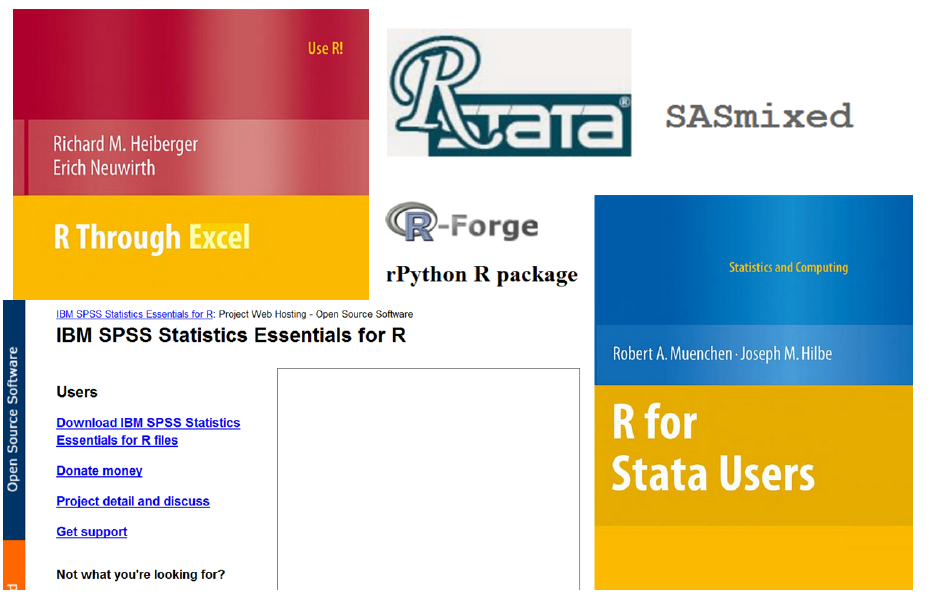
\includegraphics{figure/Rinterfaces.PNG}
\caption{}
\end{figure}

\subsection{R für SPSS Nutzer}\label{r-fur-spss-nutzer}

\begin{Shaded}
\begin{Highlighting}[]
\KeywordTok{install.packages}\NormalTok{(}\StringTok{"Rcmdr"}\NormalTok{)}
\KeywordTok{library}\NormalTok{(}\StringTok{"Rcmdr"}\NormalTok{)}
\end{Highlighting}
\end{Shaded}

Bob Munich -
\href{https://science.nature.nps.gov/im/datamgmt/statistics/r/documents/r_for_sas_spss_users.pdf}{R
for SPSS and SAS Users}

\begin{figure}[htbp]
\centering
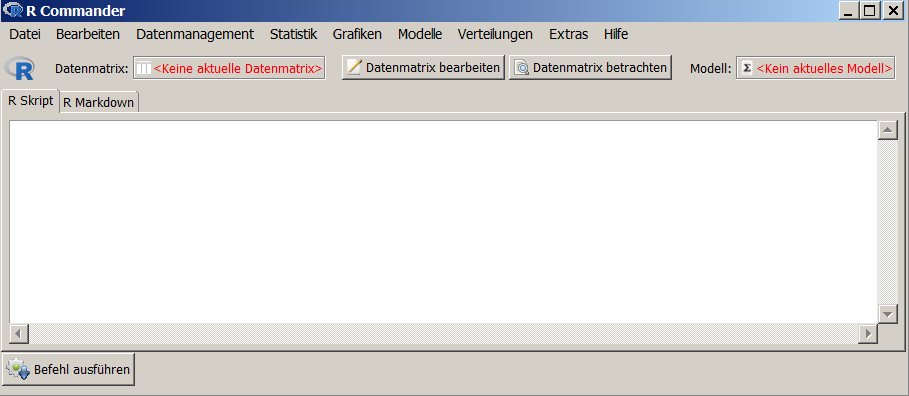
\includegraphics{figure/Rcommanderex.PNG}
\caption{}
\end{figure}

\subsection{\texorpdfstring{\href{https://gallery.shinyapps.io/cran-gauge/}{Die
Popularität von R}}{Die Popularität von R}}\label{die-popularitat-von-r}

\begin{figure}[htbp]
\centering
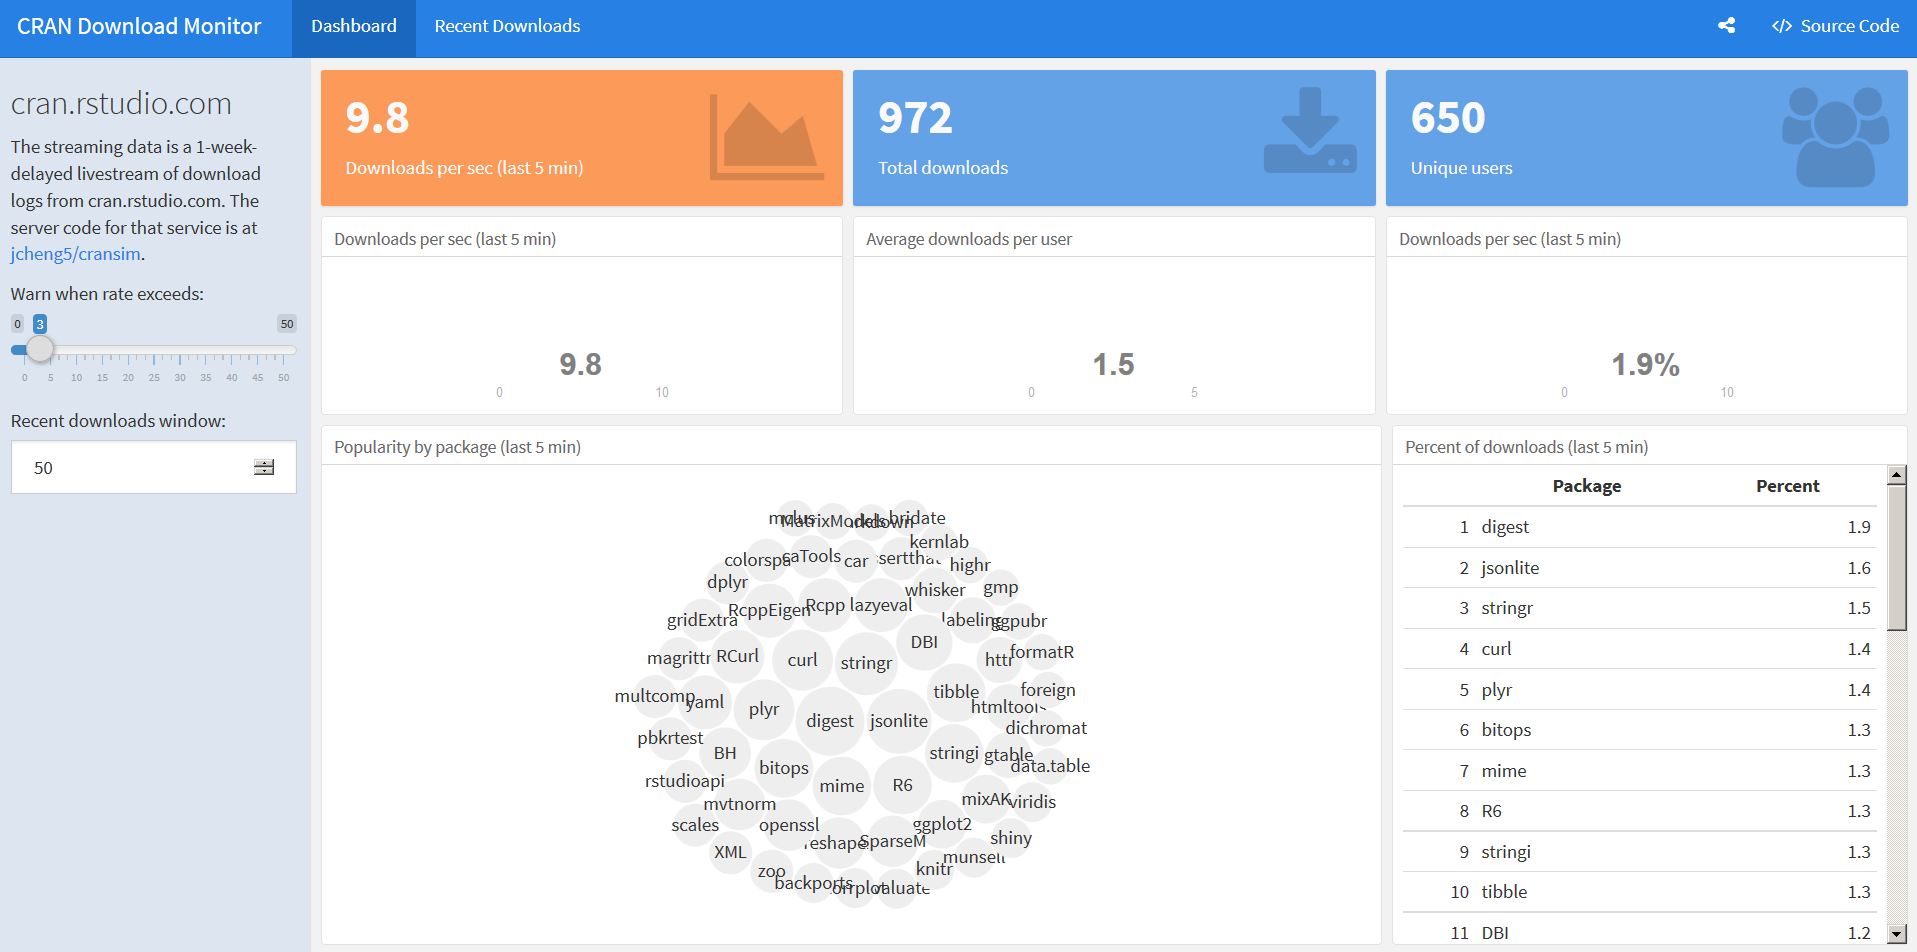
\includegraphics{figure/CRANdownloads.PNG}
\caption{}
\end{figure}

\subsection{R Nutzer rund um die Welt}\label{r-nutzer-rund-um-die-welt}

\begin{figure}[htbp]
\centering
\includegraphics{http://revolution-computing.typepad.com/.a/6a010534b1db25970b0191035099d8970c-pi}
\caption{R Welt}
\end{figure}

\subsection{Wo sind die aktivsten
Nutzer?}\label{wo-sind-die-aktivsten-nutzer}

\begin{figure}[htbp]
\centering
\includegraphics{http://spatial.ly/wp-content/uploads/2013/06/r_activity.png}
\caption{Aktivität Nutzer}
\end{figure}

\subsection{Erwartungen und
Anforderungen}\label{erwartungen-und-anforderungen}

Das kann diese Schulung vermitteln:

\begin{itemize}
\tightlist
\item
  Eine praxisnahe Einführung in die statistische Programmiersprache R
\item
  Erlernen einer Programmier-Strategie
\item
  Guten Stil
\item
  Die Vorzüge graphischer Datenanalyse
\end{itemize}

\subsection{Erwartungen und Anforderungen
II}\label{erwartungen-und-anforderungen-ii}

Das kann sie nicht leisten:

\begin{itemize}
\tightlist
\item
  Eine Einführungsveranstaltung in die Statistik geben
\item
  Grundlegende datenanalytische Konzepte vermitteln
\item
  Verständnis zementieren
\item
  Das Trainieren abnehmen
\end{itemize}

\subsection{R herunterladen:}\label{r-herunterladen}

\url{http://www.r-project.org/}

\begin{figure}[htbp]
\centering
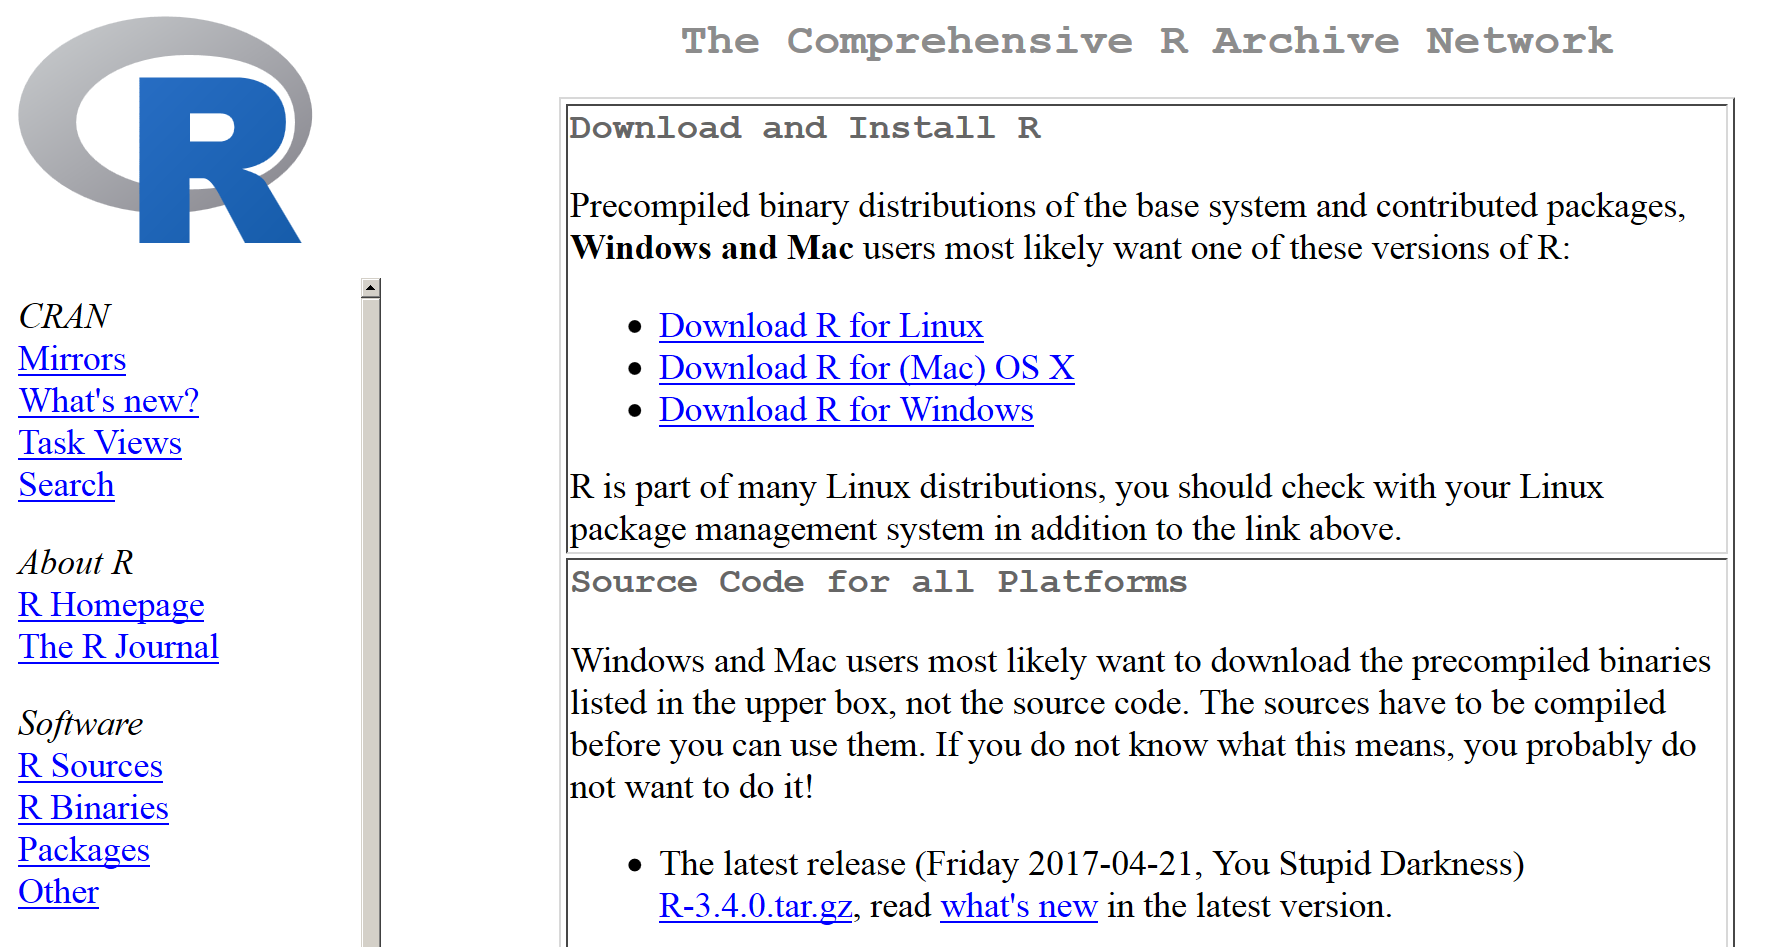
\includegraphics{figure/CRAN1picture.PNG}
\caption{}
\end{figure}

\subsection{Links}\label{links}

\begin{itemize}
\item
  \href{http://www.r-bloggers.com/why-you-should-learn-r-first-for-data-science/}{Warum
  man R für Data Science lernen sollte}
\item
  \href{http://www.r-bloggers.com/rstudio-infoworld-2015-technology-of-the-year-award-recipient/}{R
  Technologie des Jahres}
\item
  \href{http://www.fastcolabs.com/3030063/why-the-r-programming-language-is-good-for-business}{Why
  R is Good for Business}
\item
  \href{http://www.r-bloggers.com/why-use-r/}{Warum R auf r-bloggers}
\item
  \href{http://www.ats.ucla.edu/stat/r/seminars/intro.htm}{Intro R}
\item
  \href{http://www.ats.ucla.edu/stat/r/sk/}{Intro R II}
\item
  \href{http://www.dataschool.io/python-or-r-for-data-science/}{Vergleich
  python und R}
\end{itemize}

\subsection{Probleme mit Excel}\label{probleme-mit-excel}

Weil andere Programme große Fehler haben:

\begin{itemize}
\item
  \href{http://blog.revolutionanalytics.com/2013/02/did-an-excel-error-bring-down-the-london-whale.html}{Excel
  bug}
\item
  \href{https://coffeehouse.dataone.org/2014/04/09/abandon-all-hope-ye-who-enter-dates-in-excel/}{Datum
  in Excel}
\end{itemize}

\begin{figure}[htbp]
\centering

\includegraphics{figure/Abandon.PNG}
\caption{}
\end{figure}

\subsection{\texorpdfstring{\href{http://www.biomedcentral.com/1471-2105/5/80}{Probleme
mit Excel}}{Probleme mit Excel}}\label{probleme-mit-excel-1}

\begin{figure}[htbp]
\centering

\includegraphics{figure/ExcelProblems.PNG}
\caption{}
\end{figure}

\subsection{\texorpdfstring{\href{https://www.inwt-statistics.de/blog-artikel-lesen/Statistik-Software-R_SAS_SPSS_STATA_im_Vergleich.html}{Vergleich
mit anderen
Programmen}}{Vergleich mit anderen Programmen}}\label{vergleich-mit-anderen-programmen}

\begin{figure}[htbp]
\centering

\includegraphics{figure/SoftwareVergleich.PNG}
\caption{}
\end{figure}

\section{Dein Freund das GUI}\label{dein-freund-das-gui}

\subsection{Open Source Programm R}\label{open-source-programm-r}

\begin{itemize}
\item
  R ist eine freie, nicht-kommerzielle Implementierung der
  Programmiersprache S (von AT\&T Bell Laboratories entwickelt)
\item
  Freie Beteiligung - modularer Aufbau (immer mehr Erweiterungspakete)
\item
  Der Download ist auf dieser Seite möglich:
\end{itemize}

\url{https://cran.r-project.org/}

\begin{figure}[htbp]
\centering
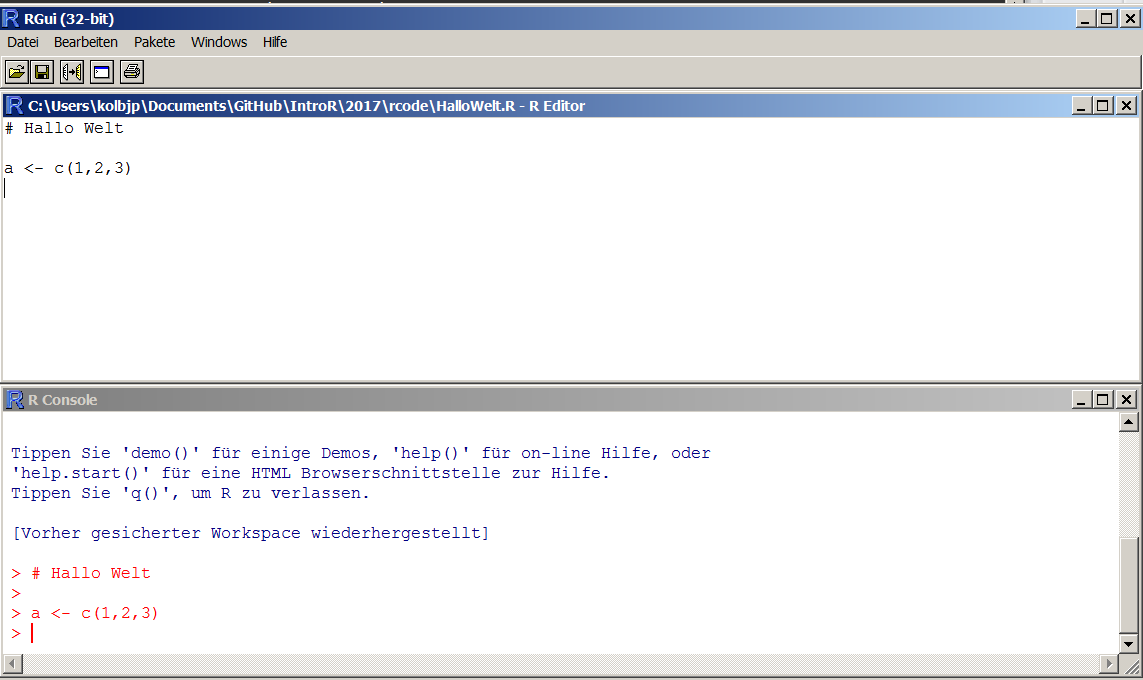
\includegraphics{figure/BasisR.PNG}
\caption{}
\end{figure}

\subsection{Graphisches User
Interface}\label{graphisches-user-interface}

Aber die meisten Menschen nutzen einen Editor oder ein graphical user
interface (GUI).

Aus den folgenden Gründen:

\begin{itemize}
\tightlist
\item
  Syntax highlighting
\item
  Auto-Vervollständigung
\item
  Bessere Übersicht über Graphiken, Bibliotheken
\end{itemize}

\subsection{Verschiedene GUIs}\label{verschiedene-guis}

\begin{itemize}
\item
  \href{https://projects.gnome.org/gedit/}{Gedit} mit R-spezifischen
  Add-ons für Linux
\item
  \href{http://www.gnu.org/software/emacs/}{Emacs}
\item
  \href{http://www.sciviews.org/Tinn-R/}{TinnR}
\item
  Ich nutze \href{https://www.rstudio.com/}{Rstudio!}
\end{itemize}

\begin{figure}[htbp]
\centering
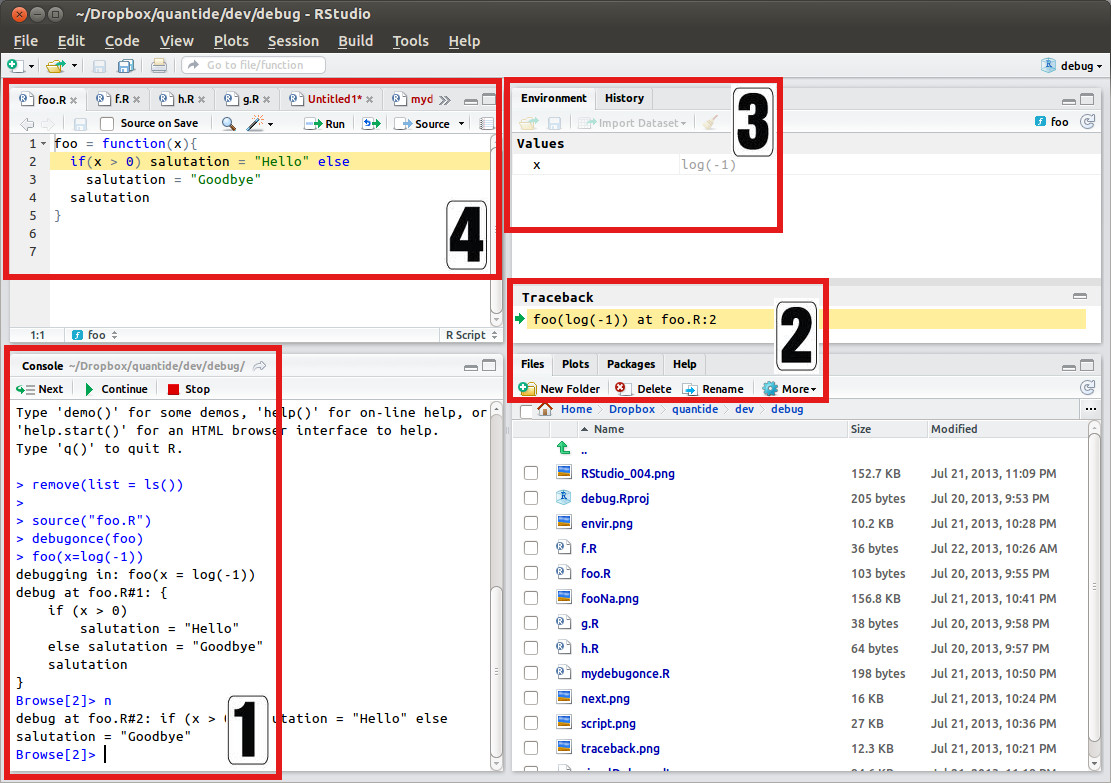
\includegraphics{http://www.milanor.net/blog/wp-content/uploads/2013/07/0_overall.jpg}
\caption{rstudio}
\end{figure}

\subsection{Rstudio}\label{rstudio}

\begin{itemize}
\item
  Sechs
  \href{http://www.r-bloggers.com/top-6-reasons-you-need-to-be-using-rstudio/}{Gründe}
  Rstudio zu nutzen.
\item
  Wie man Rstudio
  \href{https://support.rstudio.com/hc/en-us/sections/200107586-Using-RStudio}{nutzen
  kann.}
\item
  \href{https://support.rstudio.com/hc/en-us/articles/200549016-Customizing-RStudio}{Das
  Rstudio einrichten}
\end{itemize}

\subsection{Download der Unterlagen}\label{download-der-unterlagen}

Auf \href{https://github.com/Japhilko/IntroR/tree/master/2017}{github}
sind alle Unterlagen für diesen Kurs zu finden.

\href{https://guides.github.com/activities/hello-world/}{Wie nutzt man
github?}

\subsection{Aufgabe - Vorbereitung}\label{aufgabe---vorbereitung}

\begin{itemize}
\tightlist
\item
  Prüfen Sie, ob eine Version von R auf Rechner installiert ist.
\item
  Falls dies nicht der Fall ist, laden Sie \href{r-project.org}{R}
  runter und installieren Sie R.
\item
  Prüfen Sie, ob Rstudio installiert ist.
\item
  Falls nicht - \href{http://www.rstudio.com/}{Installieren} sie
  Rstudio.
\item
  Laden Sie die R-Skripte von meinem GitHub-Account
\item
  Erstellen Sie ein erstes Script und finden Sie das Datum mit dem
  Befehl \texttt{date()} und die R-version mit \texttt{sessionInfo()}
  heraus.
\end{itemize}

\begin{Shaded}
\begin{Highlighting}[]
\KeywordTok{date}\NormalTok{()}
\end{Highlighting}
\end{Shaded}

\begin{verbatim}
## [1] "Tue May 02 12:48:06 2017"
\end{verbatim}

\begin{Shaded}
\begin{Highlighting}[]
\KeywordTok{sessionInfo}\NormalTok{()}
\end{Highlighting}
\end{Shaded}

\begin{verbatim}
## R version 3.3.2 (2016-10-31)
## Platform: x86_64-w64-mingw32/x64 (64-bit)
## Running under: Windows 7 x64 (build 7601) Service Pack 1
## 
## locale:
## [1] LC_COLLATE=German_Germany.1252  LC_CTYPE=German_Germany.1252   
## [3] LC_MONETARY=German_Germany.1252 LC_NUMERIC=C                   
## [5] LC_TIME=German_Germany.1252    
## 
## attached base packages:
## [1] stats     graphics  grDevices utils     datasets  methods   base     
## 
## loaded via a namespace (and not attached):
##  [1] backports_1.0.4 magrittr_1.5    rprojroot_1.1   tools_3.3.2    
##  [5] htmltools_0.3.5 yaml_2.1.14     Rcpp_0.12.9     stringi_1.1.2  
##  [9] rmarkdown_1.3   knitr_1.15.1    stringr_1.2.0   digest_0.6.11  
## [13] evaluate_0.10
\end{verbatim}

\section{Grundlagen im Umgang mit der Sprache
R}\label{grundlagen-im-umgang-mit-der-sprache-r}

\subsection{R ist eine Objekt-orientierte
Sprache}\label{r-ist-eine-objekt-orientierte-sprache}

Vektoren und Zuweisungen

\begin{itemize}
\tightlist
\item
  R ist eine Objekt-orientierte Sprache
\item
  \texttt{\textless{}-} ist der Zuweisungsoperator
\end{itemize}

\begin{Shaded}
\begin{Highlighting}[]
\NormalTok{b <-}\StringTok{ }\KeywordTok{c}\NormalTok{(}\DecValTok{1}\NormalTok{,}\DecValTok{2}\NormalTok{) }\CommentTok{# erzeugt ein Objekt mit den Zahlen 1 und 2}
\end{Highlighting}
\end{Shaded}

\begin{itemize}
\tightlist
\item
  Eine Funktion kann auf dieses Objekt angewendet werden:
\end{itemize}

\begin{Shaded}
\begin{Highlighting}[]
\KeywordTok{mean}\NormalTok{(b) }\CommentTok{# berechnet den Mittelwert}
\end{Highlighting}
\end{Shaded}

\begin{verbatim}
## [1] 1.5
\end{verbatim}

Mit den folgenden Funktionen können wir etwas über die Eigenschaften des
Objekts lernen:

\begin{Shaded}
\begin{Highlighting}[]
\KeywordTok{length}\NormalTok{(b) }\CommentTok{# b hat die Länge 2}
\end{Highlighting}
\end{Shaded}

\begin{verbatim}
## [1] 2
\end{verbatim}

\subsection{Objektstruktur}\label{objektstruktur}

\begin{Shaded}
\begin{Highlighting}[]
\KeywordTok{str}\NormalTok{(b) }\CommentTok{# b ist ein numerischer Vektor}
\end{Highlighting}
\end{Shaded}

\begin{verbatim}
##  num [1:2] 1 2
\end{verbatim}

\subsection{Funktionen im base-Paket}\label{funktionen-im-base-paket}

\begin{longtable}[]{@{}lll@{}}
\toprule
Funktion & Bedeutung & Beispiel\tabularnewline
\midrule
\endhead
length() & Länge & length(b)\tabularnewline
max() & Maximum & max(b)\tabularnewline
min() & Minimum & min(b)\tabularnewline
sd() & Standardabweichung & sd(b)\tabularnewline
var() & Varianz & var(b)\tabularnewline
mean() & Mittelwert & mean(b)\tabularnewline
median() & Median & median(b)\tabularnewline
\bottomrule
\end{longtable}

Diese Funktionen brauchen nur ein Argument.

\subsection{Funktionen mit mehr
Argumenten}\label{funktionen-mit-mehr-argumenten}

Andere Funktionen brauchen mehr:

\begin{longtable}[]{@{}lll@{}}
\toprule
Argument & Bedeutung & Beispiel\tabularnewline
\midrule
\endhead
quantile() & 90 \% Quantile & quantile(b,.9)\tabularnewline
sample() & Stichprobe ziehen & sample(b,1)\tabularnewline
\bottomrule
\end{longtable}

\subsection{Beispiel - Funktionen mit einem
Argument}\label{beispiel---funktionen-mit-einem-argument}

\begin{Shaded}
\begin{Highlighting}[]
\KeywordTok{max}\NormalTok{(b)}
\end{Highlighting}
\end{Shaded}

\begin{verbatim}
## [1] 2
\end{verbatim}

\begin{Shaded}
\begin{Highlighting}[]
\KeywordTok{min}\NormalTok{(b)}
\end{Highlighting}
\end{Shaded}

\begin{verbatim}
## [1] 1
\end{verbatim}

\begin{Shaded}
\begin{Highlighting}[]
\KeywordTok{sd}\NormalTok{(b)}
\end{Highlighting}
\end{Shaded}

\begin{verbatim}
## [1] 0.7071068
\end{verbatim}

\begin{Shaded}
\begin{Highlighting}[]
\KeywordTok{var}\NormalTok{(b)}
\end{Highlighting}
\end{Shaded}

\begin{verbatim}
## [1] 0.5
\end{verbatim}

\subsection{Funktionen mit einem
Argument}\label{funktionen-mit-einem-argument}

\begin{Shaded}
\begin{Highlighting}[]
\KeywordTok{mean}\NormalTok{(b)}
\end{Highlighting}
\end{Shaded}

\begin{verbatim}
## [1] 1.5
\end{verbatim}

\begin{Shaded}
\begin{Highlighting}[]
\KeywordTok{median}\NormalTok{(b)}
\end{Highlighting}
\end{Shaded}

\begin{verbatim}
## [1] 1.5
\end{verbatim}

\subsection{Funktionen mit mehr
Argumenten}\label{funktionen-mit-mehr-argumenten-1}

\begin{Shaded}
\begin{Highlighting}[]
\KeywordTok{quantile}\NormalTok{(b,.}\DecValTok{9}\NormalTok{)}
\end{Highlighting}
\end{Shaded}

\begin{verbatim}
## 90% 
## 1.9
\end{verbatim}

\begin{Shaded}
\begin{Highlighting}[]
\KeywordTok{sample}\NormalTok{(b,}\DecValTok{1}\NormalTok{) }
\end{Highlighting}
\end{Shaded}

\begin{verbatim}
## [1] 2
\end{verbatim}

\subsection{\texorpdfstring{\href{http://cran.r-project.org/doc/manuals/R-intro.html}{Übersicht
Befehle}}{Übersicht Befehle}}\label{ubersicht-befehle}

\url{http://cran.r-project.org/doc/manuals/R-intro.html}

\begin{figure}[htbp]
\centering
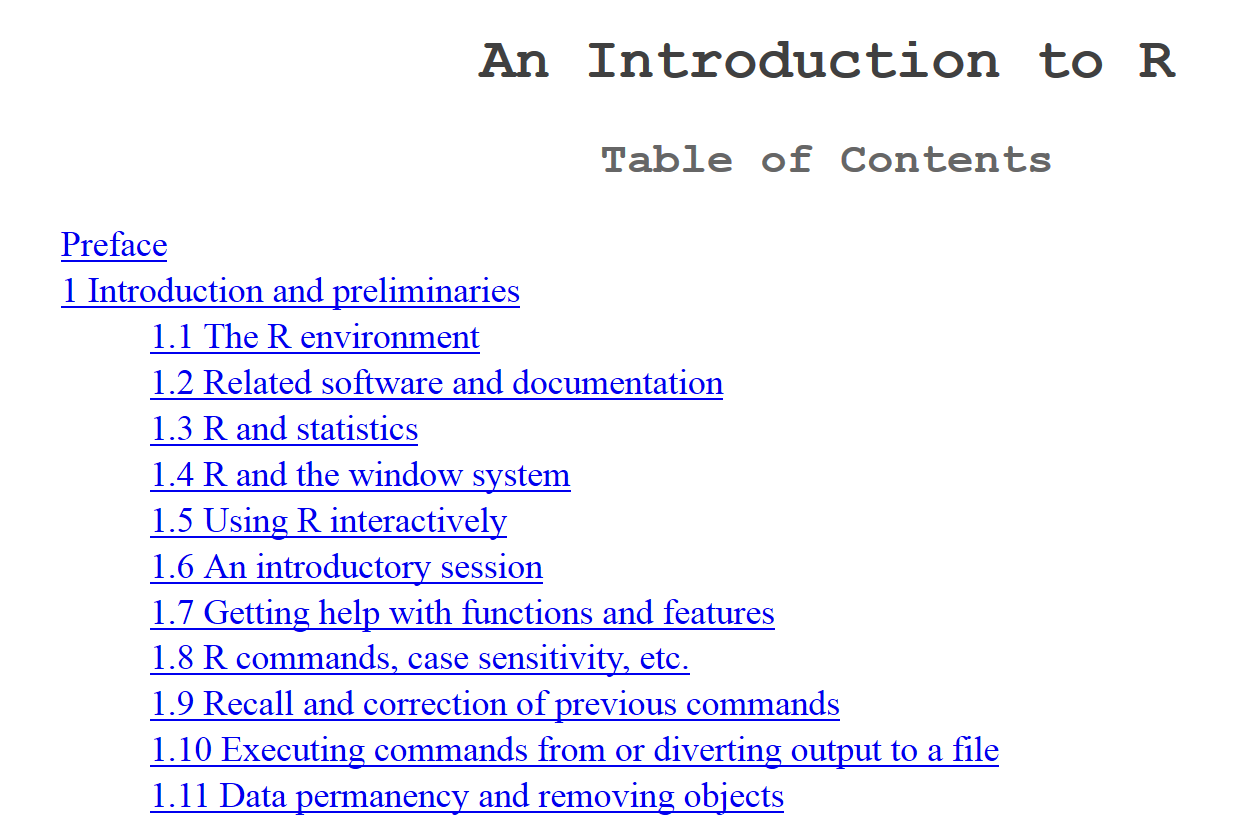
\includegraphics{figure/UebersichtBefehle.PNG}
\caption{}
\end{figure}

\subsection{Aufgabe - Zuweisungen und
Funktionen}\label{aufgabe---zuweisungen-und-funktionen}

Erzeugen Sie einen Vektor b mit den Zahlen von 1 bis 5 und berechnen
Sie\ldots{}

\begin{enumerate}
\def\labelenumi{\arabic{enumi}.}
\item
  den Mittelwert
\item
  die Varianz
\item
  die Standardabweichung
\item
  die quadratische Wurzel aus dem Mittelwert
\end{enumerate}

\section{Datentypen und Indizieren}\label{datentypen-und-indizieren}

\subsection{Verschiedene Datentypen}\label{verschiedene-datentypen}

\begin{longtable}[]{@{}lll@{}}
\toprule
Datentyp & Beschreibung & Beispiel\tabularnewline
\midrule
\endhead
numeric & ganze und reele Zahlen & 5, 3.462\tabularnewline
logical & logische Werte & FALSE, TRUE\tabularnewline
character & Buchstaben und Zeichenfolgen & ``Hallo''\tabularnewline
\bottomrule
\end{longtable}

Quelle:
\href{https://www.uni-trier.de/fileadmin/fb4/prof/VWL/FIN/Oekonometrie/PC-UEbung/Einfuehrung_in_R.pdf}{R.
Münnich und M. Knobelspieß} (2007): Einführung in das statistische
Programmpaket R

\subsection{Verschiedene Datentypen}\label{verschiedene-datentypen-1}

\begin{Shaded}
\begin{Highlighting}[]
\NormalTok{b <-}\StringTok{ }\KeywordTok{c}\NormalTok{(}\DecValTok{1}\NormalTok{,}\DecValTok{2}\NormalTok{) }\CommentTok{# numeric}
\NormalTok{log <-}\StringTok{ }\KeywordTok{c}\NormalTok{(T,F) }\CommentTok{# logical}
\NormalTok{char <-}\KeywordTok{c}\NormalTok{(}\StringTok{"A"}\NormalTok{,}\StringTok{"b"}\NormalTok{) }\CommentTok{# character}
\NormalTok{fac <-}\StringTok{ }\KeywordTok{as.factor}\NormalTok{(}\KeywordTok{c}\NormalTok{(}\DecValTok{1}\NormalTok{,}\DecValTok{2}\NormalTok{)) }\CommentTok{# factor}
\end{Highlighting}
\end{Shaded}

Mit \texttt{str()} bekommt man den Objekttyp.

\subsection{Indizieren eines Vektors:}\label{indizieren-eines-vektors}

\begin{Shaded}
\begin{Highlighting}[]
\NormalTok{A1 <-}\StringTok{ }\KeywordTok{c}\NormalTok{(}\DecValTok{1}\NormalTok{,}\DecValTok{2}\NormalTok{,}\DecValTok{3}\NormalTok{,}\DecValTok{4}\NormalTok{)}
\NormalTok{A1}
\end{Highlighting}
\end{Shaded}

\begin{verbatim}
## [1] 1 2 3 4
\end{verbatim}

\begin{Shaded}
\begin{Highlighting}[]
\NormalTok{A1[}\DecValTok{1}\NormalTok{]}
\end{Highlighting}
\end{Shaded}

\begin{verbatim}
## [1] 1
\end{verbatim}

\begin{Shaded}
\begin{Highlighting}[]
\NormalTok{A1[}\DecValTok{4}\NormalTok{]}
\end{Highlighting}
\end{Shaded}

\begin{verbatim}
## [1] 4
\end{verbatim}

\begin{Shaded}
\begin{Highlighting}[]
\NormalTok{A1[}\DecValTok{1}\NormalTok{:}\DecValTok{3}\NormalTok{]}
\end{Highlighting}
\end{Shaded}

\begin{verbatim}
## [1] 1 2 3
\end{verbatim}

\begin{Shaded}
\begin{Highlighting}[]
\NormalTok{A1[-}\DecValTok{4}\NormalTok{]}
\end{Highlighting}
\end{Shaded}

\begin{verbatim}
## [1] 1 2 3
\end{verbatim}

\subsection{data.frames}\label{data.frames}

Beispieldaten generieren:

\begin{Shaded}
\begin{Highlighting}[]
\NormalTok{AGE <-}\StringTok{ }\KeywordTok{c}\NormalTok{(}\DecValTok{20}\NormalTok{,}\DecValTok{35}\NormalTok{,}\DecValTok{48}\NormalTok{,}\DecValTok{12}\NormalTok{)}
\NormalTok{SEX <-}\StringTok{ }\KeywordTok{c}\NormalTok{(}\StringTok{"m"}\NormalTok{,}\StringTok{"w"}\NormalTok{,}\StringTok{"w"}\NormalTok{,}\StringTok{"m"}\NormalTok{)}
\end{Highlighting}
\end{Shaded}

Diese beiden Vektoren zu einem data.frame verbinden:

\begin{Shaded}
\begin{Highlighting}[]
\NormalTok{Daten <-}\StringTok{ }\KeywordTok{data.frame}\NormalTok{(}\DataTypeTok{Alter=}\NormalTok{AGE,}\DataTypeTok{Geschlecht=}\NormalTok{SEX)}
\end{Highlighting}
\end{Shaded}

Anzahl der Zeilen/Spalten herausfinden

\begin{Shaded}
\begin{Highlighting}[]
\KeywordTok{nrow}\NormalTok{(Daten) }\CommentTok{# Zeilen}
\end{Highlighting}
\end{Shaded}

\begin{verbatim}
## [1] 4
\end{verbatim}

\begin{Shaded}
\begin{Highlighting}[]
\KeywordTok{ncol}\NormalTok{(Daten) }\CommentTok{# Spalten}
\end{Highlighting}
\end{Shaded}

\begin{verbatim}
## [1] 2
\end{verbatim}

\subsection{Indizieren}\label{indizieren}

Indizieren eines dataframe:

\begin{Shaded}
\begin{Highlighting}[]
\NormalTok{AA <-}\StringTok{ }\DecValTok{4}\NormalTok{:}\DecValTok{1}
\NormalTok{A2 <-}\StringTok{ }\KeywordTok{cbind}\NormalTok{(A1,AA)}
\NormalTok{A2[}\DecValTok{1}\NormalTok{,}\DecValTok{1}\NormalTok{]}
\end{Highlighting}
\end{Shaded}

\begin{verbatim}
## A1 
##  1
\end{verbatim}

\begin{Shaded}
\begin{Highlighting}[]
\NormalTok{A2[}\DecValTok{2}\NormalTok{,]}
\end{Highlighting}
\end{Shaded}

\begin{verbatim}
## A1 AA 
##  2  3
\end{verbatim}

\begin{Shaded}
\begin{Highlighting}[]
\NormalTok{A2[,}\DecValTok{1}\NormalTok{]}
\end{Highlighting}
\end{Shaded}

\begin{verbatim}
## [1] 1 2 3 4
\end{verbatim}

\begin{Shaded}
\begin{Highlighting}[]
\NormalTok{A2[,}\DecValTok{1}\NormalTok{:}\DecValTok{2}\NormalTok{]}
\end{Highlighting}
\end{Shaded}

\begin{verbatim}
##      A1 AA
## [1,]  1  4
## [2,]  2  3
## [3,]  3  2
## [4,]  4  1
\end{verbatim}

\subsection{Matrizen und Arrays}\label{matrizen-und-arrays}

\begin{itemize}
\tightlist
\item
  In Matrizen und Arrays stehen meist nur numerische Werte.
\item
  Dadurch wird beispielsweise Matrix Multiplikation möglich.
\item
  Anders als beim data.frame sind mehr als zwei Dimensionen möglich.
\end{itemize}

\begin{Shaded}
\begin{Highlighting}[]
\NormalTok{A <-}\StringTok{ }\KeywordTok{matrix}\NormalTok{(}\KeywordTok{seq}\NormalTok{(}\DecValTok{1}\NormalTok{,}\DecValTok{100}\NormalTok{), }\DataTypeTok{nrow =} \DecValTok{4}\NormalTok{)}
\KeywordTok{dim}\NormalTok{(A)}
\end{Highlighting}
\end{Shaded}

\begin{verbatim}
## [1]  4 25
\end{verbatim}

\subsection{Ein Array erzeugen}\label{ein-array-erzeugen}

\begin{Shaded}
\begin{Highlighting}[]
\NormalTok{A3 <-}\StringTok{ }\KeywordTok{array}\NormalTok{(}\DecValTok{1}\NormalTok{:}\DecValTok{8}\NormalTok{,}\KeywordTok{c}\NormalTok{(}\DecValTok{2}\NormalTok{,}\DecValTok{2}\NormalTok{,}\DecValTok{2}\NormalTok{))}
\NormalTok{A3}
\end{Highlighting}
\end{Shaded}

\begin{verbatim}
## , , 1
## 
##      [,1] [,2]
## [1,]    1    3
## [2,]    2    4
## 
## , , 2
## 
##      [,1] [,2]
## [1,]    5    7
## [2,]    6    8
\end{verbatim}

\subsection{Indizieren eines Array}\label{indizieren-eines-array}

\begin{Shaded}
\begin{Highlighting}[]
\NormalTok{A3[,,}\DecValTok{2}\NormalTok{]}
\end{Highlighting}
\end{Shaded}

\begin{verbatim}
##      [,1] [,2]
## [1,]    5    7
## [2,]    6    8
\end{verbatim}

\subsection{Listen}\label{listen}

\begin{itemize}
\tightlist
\item
  Eine Liste in R entspricht einem geschachtelten Array in anderen
  Programmiersprachen
\item
  Listen können alles enthalten
\item
  Listen können geschachtelt sein
\item
  Listen sollte man sehr bedacht verwenden
\end{itemize}

\subsection{Indizieren einer Liste}\label{indizieren-einer-liste}

\begin{Shaded}
\begin{Highlighting}[]
\NormalTok{A4 <-}\StringTok{ }\KeywordTok{list}\NormalTok{(A1,}\DecValTok{1}\NormalTok{)}
\NormalTok{A4}
\end{Highlighting}
\end{Shaded}

\begin{verbatim}
## [[1]]
## [1] 1 2 3 4
## 
## [[2]]
## [1] 1
\end{verbatim}

\begin{Shaded}
\begin{Highlighting}[]
\NormalTok{A4[[}\DecValTok{2}\NormalTok{]]}
\end{Highlighting}
\end{Shaded}

\begin{verbatim}
## [1] 1
\end{verbatim}

\subsection{Logische Operatoren}\label{logische-operatoren}

\begin{Shaded}
\begin{Highlighting}[]
\CommentTok{# Ist 1 größer als 2?}
\DecValTok{1}\NormalTok{>}\DecValTok{2}
\end{Highlighting}
\end{Shaded}

\begin{verbatim}
## [1] FALSE
\end{verbatim}

\begin{Shaded}
\begin{Highlighting}[]
\DecValTok{1}\NormalTok{<}\DecValTok{2}
\end{Highlighting}
\end{Shaded}

\begin{verbatim}
## [1] TRUE
\end{verbatim}

\begin{Shaded}
\begin{Highlighting}[]
\DecValTok{1}\NormalTok{==}\DecValTok{2}
\end{Highlighting}
\end{Shaded}

\begin{verbatim}
## [1] FALSE
\end{verbatim}

\subsection{Operatoren um Subset für Datensatz zu
bekommen}\label{operatoren-um-subset-fur-datensatz-zu-bekommen}

Diese Operatoren eignen sich gut um Datensätze einzuschränken

\begin{Shaded}
\begin{Highlighting}[]
\NormalTok{Daten}
\end{Highlighting}
\end{Shaded}

\begin{verbatim}
##   Alter Geschlecht
## 1    20          m
## 2    35          w
## 3    48          w
## 4    12          m
\end{verbatim}

\begin{Shaded}
\begin{Highlighting}[]
\NormalTok{Daten[AGE>}\DecValTok{20}\NormalTok{,]}
\end{Highlighting}
\end{Shaded}

\begin{verbatim}
##   Alter Geschlecht
## 2    35          w
## 3    48          w
\end{verbatim}

\subsection{Datensätze einschränken}\label{datensatze-einschranken}

\begin{Shaded}
\begin{Highlighting}[]
\NormalTok{Daten[SEX==}\StringTok{"w"}\NormalTok{,]}
\end{Highlighting}
\end{Shaded}

\begin{verbatim}
##   Alter Geschlecht
## 2    35          w
## 3    48          w
\end{verbatim}

\begin{Shaded}
\begin{Highlighting}[]
\CommentTok{# gleiches Ergebnis:}
\NormalTok{Daten[SEX!=}\StringTok{"m"}\NormalTok{,]}
\end{Highlighting}
\end{Shaded}

\begin{verbatim}
##   Alter Geschlecht
## 2    35          w
## 3    48          w
\end{verbatim}

\subsection{Weitere wichtige Optionen}\label{weitere-wichtige-optionen}

\begin{Shaded}
\begin{Highlighting}[]
\CommentTok{# Ergebnis in ein Objekt speichern}
\NormalTok{subDat <-}\StringTok{ }\NormalTok{Daten[AGE>}\DecValTok{20}\NormalTok{,]}
\end{Highlighting}
\end{Shaded}

\begin{Shaded}
\begin{Highlighting}[]
\CommentTok{# mehrere Bedingeungen können mit}
\CommentTok{# & verknüpft werden:}
\NormalTok{Daten[AGE>}\DecValTok{18} \NormalTok{&}\StringTok{ }\NormalTok{SEX==}\StringTok{"w"}\NormalTok{,]}
\end{Highlighting}
\end{Shaded}

\begin{verbatim}
##   Alter Geschlecht
## 2    35          w
## 3    48          w
\end{verbatim}

\subsection{Sequenzen}\label{sequenzen}

\begin{Shaded}
\begin{Highlighting}[]
\CommentTok{# Sequenz von 1 bis 10}
\DecValTok{1}\NormalTok{:}\DecValTok{10}
\end{Highlighting}
\end{Shaded}

\begin{verbatim}
##  [1]  1  2  3  4  5  6  7  8  9 10
\end{verbatim}

\begin{Shaded}
\begin{Highlighting}[]
\NormalTok{Daten[}\DecValTok{1}\NormalTok{:}\DecValTok{3}\NormalTok{,]}
\end{Highlighting}
\end{Shaded}

\begin{verbatim}
##   Alter Geschlecht
## 1    20          m
## 2    35          w
## 3    48          w
\end{verbatim}

\subsection{Weitere Sequenzen}\label{weitere-sequenzen}

\begin{Shaded}
\begin{Highlighting}[]
\KeywordTok{seq}\NormalTok{(-}\DecValTok{2}\NormalTok{,}\DecValTok{8}\NormalTok{,}\DataTypeTok{by=}\FloatTok{1.5}\NormalTok{)}
\end{Highlighting}
\end{Shaded}

\begin{verbatim}
## [1] -2.0 -0.5  1.0  2.5  4.0  5.5  7.0
\end{verbatim}

\begin{Shaded}
\begin{Highlighting}[]
\NormalTok{a <-}\KeywordTok{seq}\NormalTok{(}\DecValTok{3}\NormalTok{,}\DecValTok{12}\NormalTok{,}\DataTypeTok{length=}\DecValTok{12}\NormalTok{)}

\NormalTok{b <-}\StringTok{ }\KeywordTok{seq}\NormalTok{(}\DataTypeTok{to=}\DecValTok{5}\NormalTok{,}\DataTypeTok{length=}\DecValTok{12}\NormalTok{,}\DataTypeTok{by=}\FloatTok{0.2}\NormalTok{)}

\NormalTok{d <-}\StringTok{ }\DecValTok{1}\NormalTok{:}\DecValTok{10}
\NormalTok{d <-}\StringTok{ }\KeywordTok{seq}\NormalTok{(}\DecValTok{1}\NormalTok{,}\DecValTok{10}\NormalTok{,}\DecValTok{1}\NormalTok{)}
\NormalTok{d <-}\StringTok{ }\KeywordTok{seq}\NormalTok{(}\DataTypeTok{length=}\DecValTok{10}\NormalTok{,}\DataTypeTok{from=}\DecValTok{1}\NormalTok{,}\DataTypeTok{by=}\DecValTok{1}\NormalTok{)}
\end{Highlighting}
\end{Shaded}

\subsection{Wiederholungen}\label{wiederholungen}

\begin{Shaded}
\begin{Highlighting}[]
\CommentTok{# wiederhole 1 10 mal}
\KeywordTok{rep}\NormalTok{(}\DecValTok{1}\NormalTok{,}\DecValTok{10}\NormalTok{)}
\end{Highlighting}
\end{Shaded}

\begin{verbatim}
##  [1] 1 1 1 1 1 1 1 1 1 1
\end{verbatim}

\begin{Shaded}
\begin{Highlighting}[]
\KeywordTok{rep}\NormalTok{(}\StringTok{"A"}\NormalTok{,}\DecValTok{10}\NormalTok{)}
\end{Highlighting}
\end{Shaded}

\begin{verbatim}
##  [1] "A" "A" "A" "A" "A" "A" "A" "A" "A" "A"
\end{verbatim}

\subsection{Die Funktion paste}\label{die-funktion-paste}

\begin{Shaded}
\begin{Highlighting}[]
\NormalTok{?paste}
\end{Highlighting}
\end{Shaded}

\begin{Shaded}
\begin{Highlighting}[]
\KeywordTok{paste}\NormalTok{(}\DecValTok{1}\NormalTok{:}\DecValTok{4}\NormalTok{)}
\end{Highlighting}
\end{Shaded}

\begin{verbatim}
## [1] "1" "2" "3" "4"
\end{verbatim}

\begin{Shaded}
\begin{Highlighting}[]
\KeywordTok{paste}\NormalTok{(}\StringTok{"A"}\NormalTok{, }\DecValTok{1}\NormalTok{:}\DecValTok{6}\NormalTok{, }\DataTypeTok{sep =} \StringTok{""}\NormalTok{)}
\end{Highlighting}
\end{Shaded}

\begin{verbatim}
## [1] "A1" "A2" "A3" "A4" "A5" "A6"
\end{verbatim}

\section{Wie bekommt man Hilfe?}\label{wie-bekommt-man-hilfe}

\subsection{Wie bekommt man Hilfe?}\label{wie-bekommt-man-hilfe-1}

\begin{itemize}
\tightlist
\item
  \href{http://itfeature.com/tag/how-to-get-help-in-r}{Um generell Hilfe
  zu bekommen:}
\end{itemize}

\begin{Shaded}
\begin{Highlighting}[]
\KeywordTok{help.start}\NormalTok{()}
\end{Highlighting}
\end{Shaded}

\begin{itemize}
\tightlist
\item
  Online Dokumentation für die meisten Funktionen:
\end{itemize}

\begin{Shaded}
\begin{Highlighting}[]
\KeywordTok{help}\NormalTok{(name)}
\end{Highlighting}
\end{Shaded}

\begin{itemize}
\tightlist
\item
  Nutze ? um Hilfe zu bekommen.
\end{itemize}

\begin{Shaded}
\begin{Highlighting}[]
\NormalTok{?mean}
\end{Highlighting}
\end{Shaded}

\begin{itemize}
\tightlist
\item
  example(lm) gibt ein Beispiel für die lineare Regression
\end{itemize}

\begin{Shaded}
\begin{Highlighting}[]
\KeywordTok{example}\NormalTok{(lm)}
\end{Highlighting}
\end{Shaded}

\subsection{Nutzung Suchmaschinen}\label{nutzung-suchmaschinen}

\begin{itemize}
\tightlist
\item
  Ich nutze meistens google
\item
  Tippe:
\end{itemize}

\begin{verbatim}
R-project + Was ich schon immer wissen wollte
\end{verbatim}

\begin{itemize}
\tightlist
\item
  Das funktioniert natürlich mit jeder Suchmaschine!
\end{itemize}

\subsection{\texorpdfstring{\href{http://stackoverflow.com/}{Stackoverflow}}{Stackoverflow}}\label{stackoverflow}

\begin{itemize}
\tightlist
\item
  Für Fragen zum Programmieren
\item
  Ist nicht auf R fokussiert
\item
  Sehr detailierte Diskussionen
\end{itemize}

\begin{figure}[htbp]
\centering
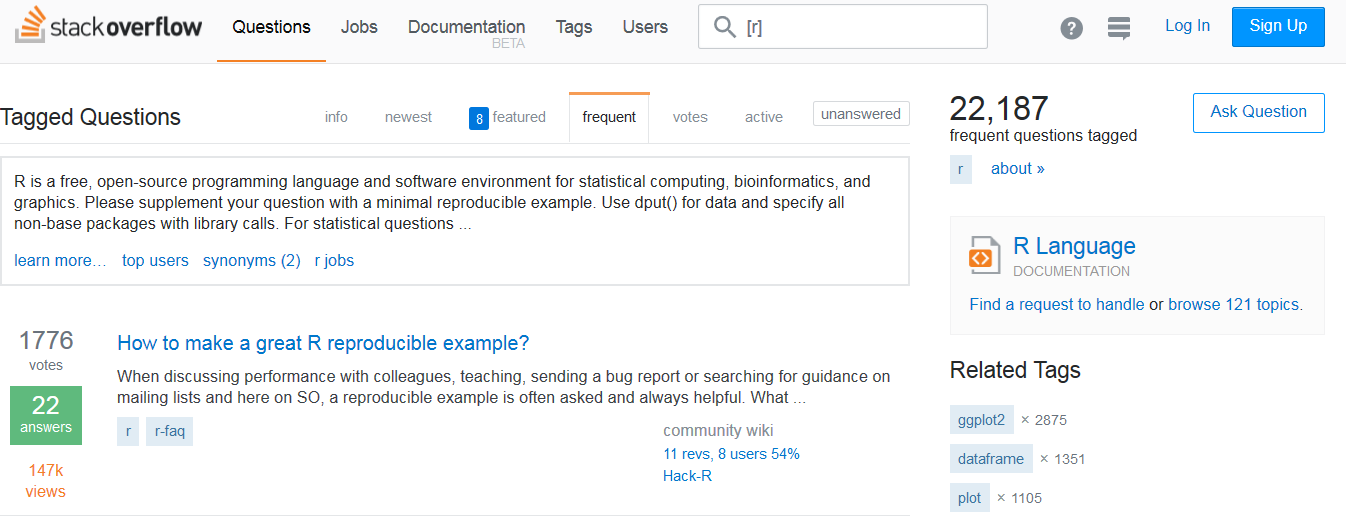
\includegraphics{https://github.com/Japhilko/IntroR/blob/master/2017/slides/figure/StackoverflowEx.PNG?raw=true}
\caption{}
\end{figure}

\subsection{Ein Schummelzettel -
Cheatsheet}\label{ein-schummelzettel---cheatsheet}

\url{https://www.rstudio.com/resources/cheatsheets/}

\begin{figure}[htbp]
\centering
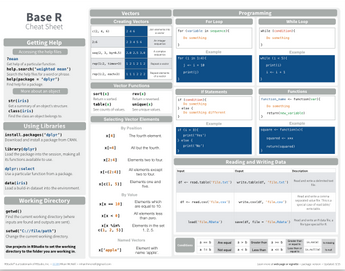
\includegraphics{https://github.com/Japhilko/IntroR/blob/master/2017/slides/figure/cheatsheetBaseR.PNG?raw=true}
\caption{}
\end{figure}

\section{Modularer Aufbau von R}\label{modularer-aufbau-von-r}

\subsection{Modularer Aufbau}\label{modularer-aufbau}

\begin{figure}[htbp]
\centering
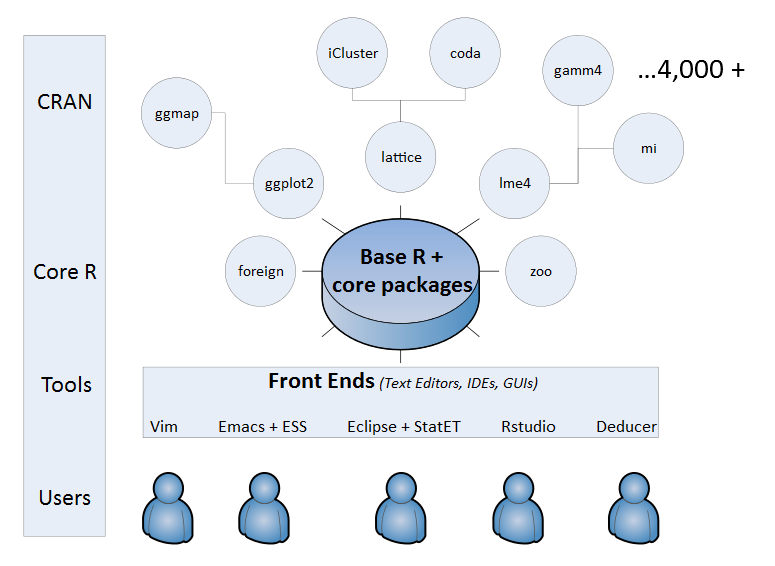
\includegraphics{figure/Packages.PNG}
\caption{}
\end{figure}

\subsection{Modularer Aufbau}\label{modularer-aufbau-1}

\begin{itemize}
\tightlist
\item
  Viele Funktionen sind im Basis-R enthalten
\item
  Viele spezifische Funktionen sind in zusätzlichen Bibliotheken
  integriert
\item
  R kann modular erweitert werden durch sog. packages bzw. libraries
\item
  Auf CRAN werden die wichtigsten packages gehostet (im Moment 10430)
\item
  Weitergehende Pakete finden sich z.B. bei
  \href{www.bioconductor.org}{bioconductor}
\end{itemize}

\begin{Shaded}
\begin{Highlighting}[]
\KeywordTok{install.packages}\NormalTok{(}\StringTok{"lme4"}\NormalTok{)}

\KeywordTok{library}\NormalTok{(lme4)}
\end{Highlighting}
\end{Shaded}

\subsection{Installation von Paketen mit
RStudio}\label{installation-von-paketen-mit-rstudio}

\begin{figure}[htbp]
\centering
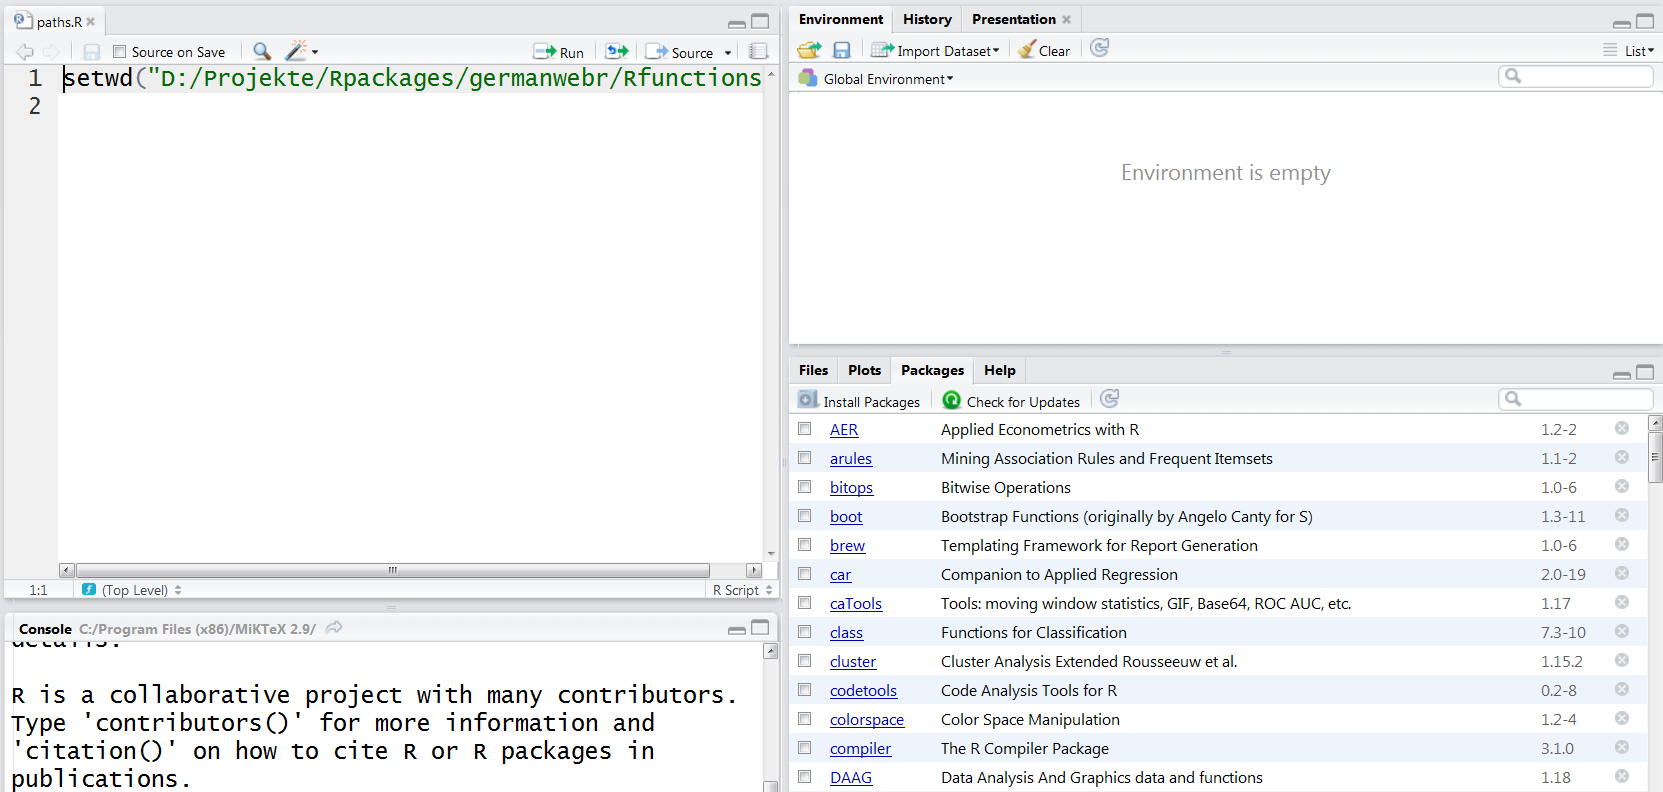
\includegraphics{https://github.com/Japhilko/IntroR/blob/master/2017/slides/figure/PaketeRstudio.PNG?raw=true}
\caption{}
\end{figure}

\subsection{Vorhandene Pakete und
Installation}\label{vorhandene-pakete-und-installation}

\begin{figure}[htbp]
\centering
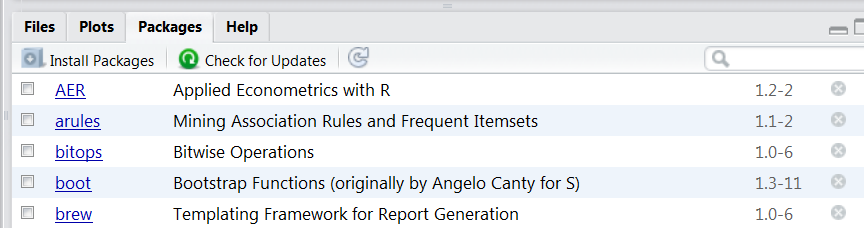
\includegraphics{https://github.com/Japhilko/IntroR/blob/master/2017/slides/figure/packages3.PNG?raw=true}
\caption{}
\end{figure}

\subsection{Übersicht viele nützliche
Pakete:}\label{ubersicht-viele-nutzliche-pakete}

\begin{itemize}
\tightlist
\item
  Luhmann -
  \href{http://www.beltz.de/fileadmin/beltz/downloads/OnlinematerialienPVU/28090_Luhmann/Verwendete\%20Pakete.pdf}{Tabelle
  mit vielen nützlichen Paketen}
\end{itemize}

Die wichtigsten Pakete zur Visualisierung mit R:

\begin{itemize}
\tightlist
\item
  \href{http://ggplot2.org/}{ggplot}
\item
  \href{http://lattice.r-forge.r-project.org/Vignettes/src/lattice-intro/lattice-intro.pdf}{lattice}
\item
  \href{http://www.statmethods.net/advgraphs/mosaic.html}{Visualisierung
  kategorialer Daten}
\item
  \href{http://cran.r-project.org/web/packages/googleVis/vignettes/googleVis_examples.html}{Interaktive
  Visualisierungen}
\item
  \href{http://www.inside-r.org/packages/cran/plotrix/docs/draw.circle}{plotrix}
\item
  \href{http://cran.r-project.org/web/packages/colorspace/vignettes/hcl-colors.pdf}{Farbpaletten
  in R}
\end{itemize}

\subsection{Pakete Regression}\label{pakete-regression}

\begin{itemize}
\item
  \href{http://cran.r-project.org/web/packages/MASS/MASS.pdf}{R-Paket
  MASS}
\item
  \href{http://cran.r-project.org/web/packages/tsDyn/vignettes/tsDyn.pdf}{Autoregressive
  Modelle (Zeitreihen)}
\item
  \href{http://robustbase.r-forge.r-project.org/}{Robuste Regressionen}
\item
  \href{http://journal.r-project.org/archive/2012-2/RJournal_2012-2_Nie+S~Racine.pdf}{Nichtparametrische
  Regression}
\item
  \href{http://web.stanford.edu/~hastie/glmnet/glmnet_alpha.html}{Lasso
  Verfahren}
\end{itemize}

\subsection{Big Data}\label{big-data}

\begin{itemize}
\tightlist
\item
  \href{http://cran.r-project.org/web/views/HighPerformanceComputing.html}{Task
  View - High Performance Computing}
\end{itemize}

Weitere interessante Pakete

Paket für den Import/Export -
\href{http://cran.r-project.org/web/packages/foreign/foreign.pdf}{foreign}

\begin{itemize}
\item
  \href{http://iase-web.org/documents/papers/icots8/ICOTS8_4J1_TILLE.pdf}{Pakete
  für Survey Sampling}
\item
  Paket - Latex und R (xtable)
  (\href{http://cran.r-project.org/web/packages/xtable/vignettes/xtableGallery.pdf}{xtable
  Galerie})
\item
  \href{http://cran.r-project.org/web/packages/dummies/dummies.pdf}{Paket
  zur Erzeugung von Dummies}
\item
  \href{http://cran.r-project.org/web/packages/mvtnorm/index.html}{Multivariate
  Normalverteilung}
\item
  \href{http://www.r-bloggers.com/tag/maptools/}{Paket für Karten}
\end{itemize}

\subsection{Pakete von Github
installieren}\label{pakete-von-github-installieren}

\begin{Shaded}
\begin{Highlighting}[]
\KeywordTok{install.packages}\NormalTok{(}\StringTok{"devtools"}\NormalTok{)}
\KeywordTok{library}\NormalTok{(devtools)}

\KeywordTok{install_github}\NormalTok{(}\StringTok{"hadley/ggplot2"}\NormalTok{)}
\end{Highlighting}
\end{Shaded}

\subsection{Wie bekomme ich einen
Überblick}\label{wie-bekomme-ich-einen-uberblick}

\begin{itemize}
\item
  \href{https://mran.microsoft.com/packages/}{Explore Packages Currently
  on CRAN}
\item
  \href{https://gallery.shinyapps.io/cran-gauge/}{Pakete die in letzter
  Zeit von CRAN heruntergeladen wurden}
\end{itemize}

\subsection{Aufgabe - Zusatzpakete}\label{aufgabe---zusatzpakete}

Gehen Sie auf \textless{}cran.r-project.org\textgreater{} und suchen Sie
in dem Bereich, wo die Pakete vorgestellt werden, nach Paketen,\ldots{}

\begin{itemize}
\tightlist
\item
  die für die deskriptive Datenanalyse geeignet sind.
\item
  um Regressionen zu berechnen
\item
  um fremde Datensätze einzulesen (z.B. SPSS-Daten)
\item
  um mit großen Datenmengen umzugehen
\end{itemize}

\section{Datenimport}\label{datenimport}

\subsection{Datenimport}\label{datenimport-1}

\begin{figure}[htbp]
\centering
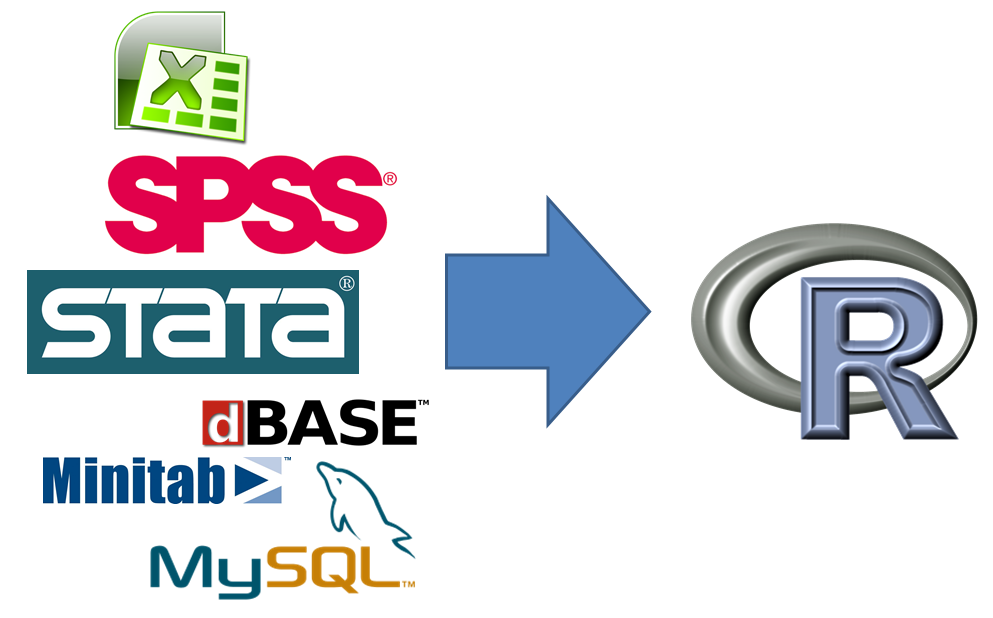
\includegraphics{figure/Datenimport.PNG}
\caption{}
\end{figure}

\subsection{Dateiformate in R}\label{dateiformate-in-r}

\begin{itemize}
\tightlist
\item
  Von R werden quelloffene, nicht-proprietäre Formate bevorzugt
\item
  Es können aber auch Formate von anderen Statistik Software Paketen
  eingelesen werden
\item
  R-user speichern Objekte gerne in sog. Workspaces ab
\item
  Auch hier jedoch gilt: (fast) alles andere ist möglich
\end{itemize}

\subsection{Formate - base package}\label{formate---base-package}

R unterstützt von Haus aus schon einige wichtige Formate:

\begin{itemize}
\tightlist
\item
  CSV (Comma Separated Values): \texttt{read.csv()}
\item
  FWF (Fixed With Format): \texttt{read.fwf()}
\item
  Tab-getrennte Werte: \texttt{read.delim()}
\end{itemize}

\subsection{Der Arbeitsspeicher}\label{der-arbeitsspeicher}

So findet man heraus, in welchem Verzeichnis man sich gerade befindet

\begin{Shaded}
\begin{Highlighting}[]
\KeywordTok{getwd}\NormalTok{()}
\end{Highlighting}
\end{Shaded}

So kann man das Arbeitsverzeichnis ändern:

Man erzeugt ein Objekt in dem man den Pfad abspeichert:

\begin{Shaded}
\begin{Highlighting}[]
\NormalTok{main.path <-}\StringTok{ "C:/"} \CommentTok{# Beispiel für Windows}
\NormalTok{main.path <-}\StringTok{ "/users/Name/"} \CommentTok{# Beispiel für Mac}
\NormalTok{main.path <-}\StringTok{ "/home/user/"} \CommentTok{# Beispiel für Linux}
\end{Highlighting}
\end{Shaded}

Und ändert dann den Pfad mit setwd()

\begin{Shaded}
\begin{Highlighting}[]
\KeywordTok{setwd}\NormalTok{(main.path)}
\end{Highlighting}
\end{Shaded}

Bei Windows ist es wichtig Slashs anstelle von Backslashs zu verwenden.

\subsection{Alternative -
Arbeitsspeicher}\label{alternative---arbeitsspeicher}

\begin{figure}[htbp]
\centering
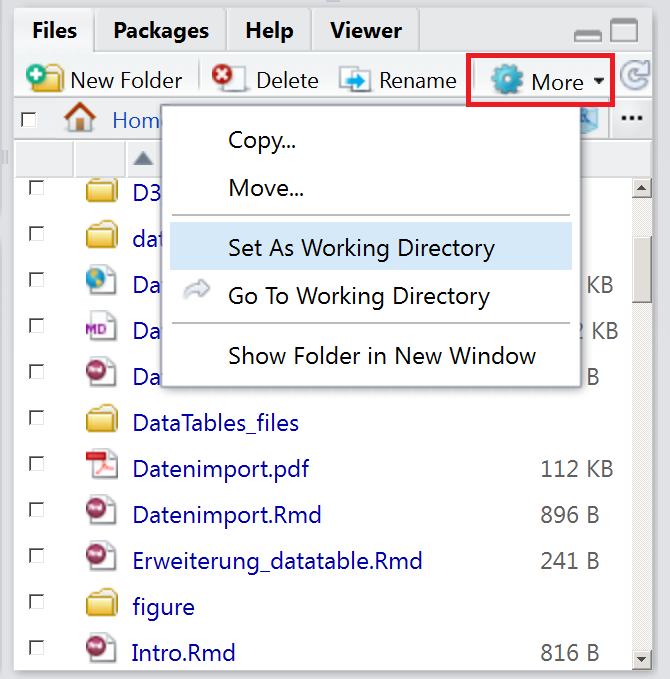
\includegraphics{figure/SetWD.PNG}
\caption{}
\end{figure}

\subsection{Import von Excel-Daten}\label{import-von-excel-daten}

\begin{itemize}
\tightlist
\item
  \texttt{library(foreign)} ist für den Import von fremden Datenformaten
  nötig
\item
  Wenn Excel-Daten vorliegen - als .csv abspeichern
\item
  Dann kann \texttt{read.csv()} genutzt werden um die Daten einzulesen.
\item
  Bei Deutschen Daten kann es sein, dass man \texttt{read.csv2()} wegen
  der Komma-Separierung braucht.
\end{itemize}

\begin{Shaded}
\begin{Highlighting}[]
\KeywordTok{library}\NormalTok{(foreign)}
\NormalTok{?read.csv}
\NormalTok{?read.csv2}
\end{Highlighting}
\end{Shaded}

\subsection{CSV Dateien einlesen}\label{csv-dateien-einlesen}

Zunächst muss das Arbeitsverzeichnis gesetzt werden, in dem sich die
Daten befinden:

\begin{Shaded}
\begin{Highlighting}[]
\NormalTok{Dat <-}\StringTok{ }\KeywordTok{read.csv}\NormalTok{(}\StringTok{"schuldaten_export.csv"}\NormalTok{)}
\end{Highlighting}
\end{Shaded}

Wenn es sich um Deutsche Daten handelt:

\begin{Shaded}
\begin{Highlighting}[]
\NormalTok{Dat <-}\StringTok{ }\KeywordTok{read.csv2}\NormalTok{(}\StringTok{"schuldaten_export.csv"}\NormalTok{)}
\end{Highlighting}
\end{Shaded}

\subsection{SPSS Dateien einlesen}\label{spss-dateien-einlesen}

Dateien können auch direkt aus dem Internet geladen werden:

\begin{Shaded}
\begin{Highlighting}[]
\NormalTok{link<-}\StringTok{ "http://www.statistik.at/web_de/static/}
\StringTok{mz_2013_sds_-_datensatz_080469.sav"}

\NormalTok{?read.spss}
\NormalTok{Dat <-}\StringTok{ }\KeywordTok{read.spss}\NormalTok{(link,}\DataTypeTok{to.data.frame=}\NormalTok{T)}
\end{Highlighting}
\end{Shaded}

\subsection{stata Dateien einlesen}\label{stata-dateien-einlesen}

\begin{Shaded}
\begin{Highlighting}[]
\NormalTok{MZ02 <-}\StringTok{ }\KeywordTok{read.dta}\NormalTok{(}\StringTok{"MZ02.dta"}\NormalTok{)}
\end{Highlighting}
\end{Shaded}

\begin{itemize}
\tightlist
\item
  Einführung in Import mit R
  (\href{http://is-r.tumblr.com/post/37181850668/reading-writing-stata-dta-files-with-foreign}{is.R})
\end{itemize}

\subsection{\texorpdfstring{\href{https://cran.r-project.org/web/packages/rio/vignettes/rio.html}{Das
Paket \texttt{rio}}}{Das Paket rio}}\label{das-paket-rio}

\begin{Shaded}
\begin{Highlighting}[]
\KeywordTok{install.packages}\NormalTok{(}\StringTok{"rio"}\NormalTok{)}
\end{Highlighting}
\end{Shaded}

\begin{Shaded}
\begin{Highlighting}[]
\KeywordTok{library}\NormalTok{(}\StringTok{"rio"}\NormalTok{)}
\NormalTok{x <-}\StringTok{ }\KeywordTok{import}\NormalTok{(}\StringTok{"mtcars.csv"}\NormalTok{)}
\NormalTok{y <-}\StringTok{ }\KeywordTok{import}\NormalTok{(}\StringTok{"mtcars.rds"}\NormalTok{)}
\NormalTok{z <-}\StringTok{ }\KeywordTok{import}\NormalTok{(}\StringTok{"mtcars.dta"}\NormalTok{)}
\end{Highlighting}
\end{Shaded}

\begin{itemize}
\tightlist
\item
  \href{https://cran.r-project.org/web/packages/rio/README.html}{rio: A
  Swiss-Army Knife for Data I/O}
\end{itemize}

\subsection{Datenmanagement ähnlich wie in SPSS oder
Stata}\label{datenmanagement-ahnlich-wie-in-spss-oder-stata}

\begin{Shaded}
\begin{Highlighting}[]
\KeywordTok{install.packages}\NormalTok{(}\StringTok{"Rz"}\NormalTok{)}
\KeywordTok{library}\NormalTok{(Rz)}
\end{Highlighting}
\end{Shaded}

\subsection{\texorpdfstring{\href{https://cran.r-project.org/web/packages/Rcmdr/index.html}{Weitere
Alternative
Rcmdr}}{Weitere Alternative Rcmdr}}\label{weitere-alternative-rcmdr}

\begin{Shaded}
\begin{Highlighting}[]
\KeywordTok{install.packages}\NormalTok{(}\StringTok{"Rcmdr"}\NormalTok{)}
\end{Highlighting}
\end{Shaded}

\begin{itemize}
\tightlist
\item
  \href{http://www.rcommander.com/}{Funktioniert auch mit Rstudio}
\end{itemize}

\begin{Shaded}
\begin{Highlighting}[]
\KeywordTok{library}\NormalTok{(Rcmdr)}
\end{Highlighting}
\end{Shaded}

\begin{figure}[htbp]
\centering
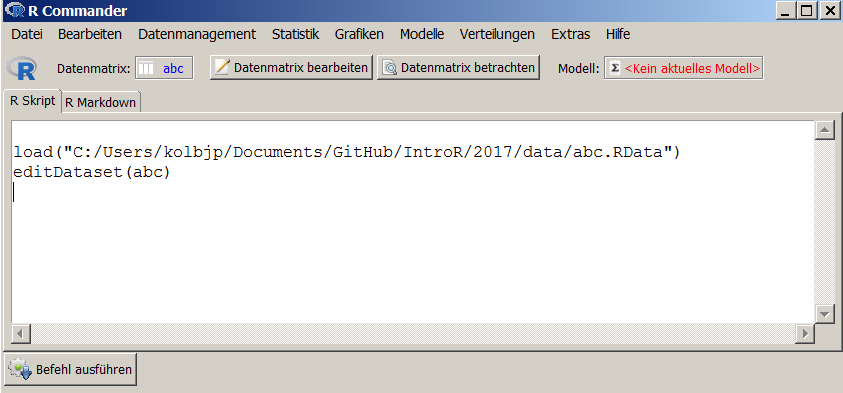
\includegraphics{figure/Rcommander.PNG}
\caption{}
\end{figure}

\subsection{Aufgabe - Datenimport}\label{aufgabe---datenimport}

\begin{itemize}
\item
  Gehen Sie auf
  \href{https://github.com/Japhilko/IntroR/blob/master/2017/data/oecd.dta?raw=true}{meine
  Github Seite} und laden Sie den OECD Datensatz herunter
\item
  Laden Sie den Datensatz mit einer geeigneten Funktion in Ihre Console.
\item
  Finden Sie heraus, wieviele Beobachtungen und Variablen der Datensatz
  umfasst.
\end{itemize}

\section{Datenexport}\label{datenexport}

\subsection{Datenexport}\label{datenexport-1}

\begin{figure}[htbp]
\centering
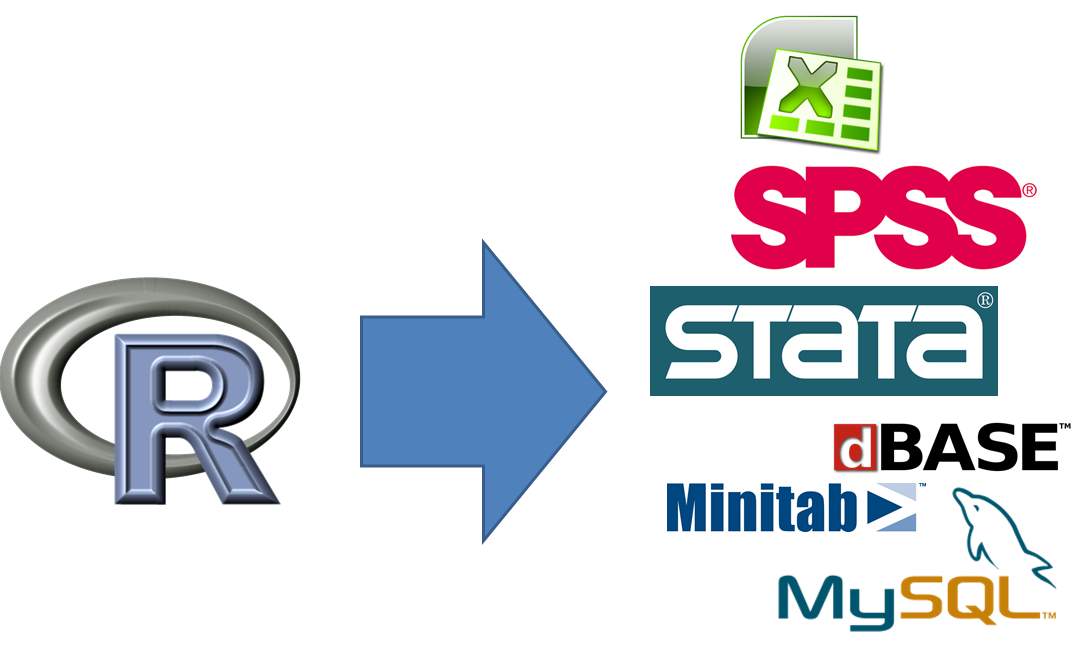
\includegraphics{figure/Datenexport.PNG}
\caption{}
\end{figure}

\subsection{R's Exportformate}\label{rs-exportformate}

\begin{itemize}
\tightlist
\item
  In R werden offene Dateiformate bevorzugt
\item
  Als Äquivalenz zu den \texttt{read.X()} Funktionen stehen viele
  \texttt{write.X()} Funktionen zur Verfügung
\item
  Das eigene Format von R sind sog. Workspaces (\texttt{.RData})
\end{itemize}

\subsection{Beispieldatensatz
erzeugen}\label{beispieldatensatz-erzeugen}

\begin{Shaded}
\begin{Highlighting}[]
\NormalTok{A <-}\StringTok{ }\KeywordTok{c}\NormalTok{(}\DecValTok{1}\NormalTok{,}\DecValTok{2}\NormalTok{,}\DecValTok{3}\NormalTok{,}\DecValTok{4}\NormalTok{)}
\NormalTok{B <-}\StringTok{ }\KeywordTok{c}\NormalTok{(}\StringTok{"A"}\NormalTok{,}\StringTok{"B"}\NormalTok{,}\StringTok{"C"}\NormalTok{,}\StringTok{"D"}\NormalTok{)}

\NormalTok{mydata <-}\StringTok{ }\KeywordTok{data.frame}\NormalTok{(A,B)}
\end{Highlighting}
\end{Shaded}

\subsection{Überblick Daten
Import/Export}\label{uberblick-daten-importexport}

\begin{Shaded}
\begin{Highlighting}[]
\KeywordTok{save}\NormalTok{(mydata, }\DataTypeTok{file=}\StringTok{"mydata.RData"}\NormalTok{)}
\end{Highlighting}
\end{Shaded}

\subsection{Daten in Excel Format
abspeichern}\label{daten-in-excel-format-abspeichern}

\begin{Shaded}
\begin{Highlighting}[]
\KeywordTok{write.csv}\NormalTok{(mydata,}\DataTypeTok{file=}\StringTok{"mydata.csv"}\NormalTok{) }
\end{Highlighting}
\end{Shaded}

\begin{Shaded}
\begin{Highlighting}[]
\KeywordTok{library}\NormalTok{(xlsx)}
\KeywordTok{write.xlsx}\NormalTok{(mydata,}\DataTypeTok{file=}\StringTok{"mydata.xlsx"}\NormalTok{) }
\end{Highlighting}
\end{Shaded}

\subsection{Daten in stata Format
abspeichern}\label{daten-in-stata-format-abspeichern}

\begin{Shaded}
\begin{Highlighting}[]
\KeywordTok{library}\NormalTok{(foreign)}
\KeywordTok{write.dta}\NormalTok{(mydata,}\DataTypeTok{file=}\StringTok{"mydata.dta"}\NormalTok{) }
\end{Highlighting}
\end{Shaded}

\subsection{\texorpdfstring{Auch zum Export eignet sich das \texttt{rio}
Paket}{Auch zum Export eignet sich das rio Paket}}\label{auch-zum-export-eignet-sich-das-rio-paket}

\begin{Shaded}
\begin{Highlighting}[]
\KeywordTok{library}\NormalTok{(}\StringTok{"rio"}\NormalTok{)}

\KeywordTok{export}\NormalTok{(mtcars, }\StringTok{"mtcars.csv"}\NormalTok{)}
\KeywordTok{export}\NormalTok{(mtcars, }\StringTok{"mtcars.rds"}\NormalTok{)}
\KeywordTok{export}\NormalTok{(mtcars, }\StringTok{"mtcars.dta"}\NormalTok{)}
\end{Highlighting}
\end{Shaded}

\subsection{Links Export}\label{links-export}

\begin{itemize}
\item
  \href{http://www.statmethods.net/input/exportingdata.html}{Quick R}
  für das Exportieren von Daten:
\item
  Hilfe zum Export auf dem
  \href{http://cran.r-project.org/doc/manuals/r-release/R-data.pdf}{cran
  Server}
\item
  \href{https://github.com/Japhilko/IntroR/blob/master/2016/README.md}{Zurück
  zur Gliederung.}
\end{itemize}

\section{Exkurs: Datenquellen}\label{exkurs-datenquellen}

\subsection{Datenzugang}\label{datenzugang}

\begin{itemize}
\item
  Public-Use-File (PUF) Datei zur öffentlichen Nutzung - meist stark
  anonymisierte Daten (Beispiele:
  \href{www.forschungsdatenzentrum.de}{FDZ},
  \href{www.statistik-portal.de}{Statistik Portal},
  \href{www.infothek.statistik.rlp.de/lis/MeineRegion/index.asp}{Meine
  Region} )
\item
  Scientific-Use-File (SUF) - Datei zur wissenschaftlichen Nutzung -
  anonymisierte Daten, die zu wissenschaftlichen Zwecken und zur
  Sekundäranalyse genutzt werden können.
\item
  On-Site-Nutzung - Arbeitsplätze für Gastwissenschaftler -
  Kontrollierte Datenfernverarbeitung
\end{itemize}

\subsection{Datenquellen}\label{datenquellen}

\begin{itemize}
\item
  Auf dem Portal \href{http://datahub.io/}{datahub.io} sind sehr viele
  Beispieldatensätze in verschiedenen Formaten abrufbar.
\item
  Weitere Portale: \href{http://ropengov.github.io/projects/}{OpenGov},
  \href{http://data.okfn.org/}{okfn},
  \href{https://app.enigma.io/table/org.worldbank.hnp.data}{enigma},
  Amazon Web Services
  (\href{http://aws.amazon.com/de/public-data-sets/}{AWS})
\item
  Umweltdaten
  (\href{http://www.ncdc.noaa.gov/ibtracs/index.php?name=ibtracs-data}{National
  climatic data center})
\item
  \href{http://cran.r-project.org/web/packages/FAOSTAT/index.html}{FAO
  Datenbank}
\end{itemize}

\begin{Shaded}
\begin{Highlighting}[]
\KeywordTok{library}\NormalTok{(}\StringTok{"FAOSTAT"}\NormalTok{)}
\end{Highlighting}
\end{Shaded}

\begin{itemize}
\item
  Public Use File für Soziales in den USA
  \href{http://www.ssa.gov/policy/docs/data/index.html}{Social security
  administration}
\item
  National health and nutrition examination survey
\end{itemize}

\begin{Shaded}
\begin{Highlighting}[]
\KeywordTok{library}\NormalTok{(survey)}
\KeywordTok{data}\NormalTok{(nhanes)}
\end{Highlighting}
\end{Shaded}

\subsection{Das R-Paket datasets}\label{das-r-paket-datasets}

\begin{Shaded}
\begin{Highlighting}[]
\KeywordTok{library}\NormalTok{(datasets)}
\end{Highlighting}
\end{Shaded}

Beispiel Erdbeben Datensatz:

\begin{Shaded}
\begin{Highlighting}[]
\KeywordTok{head}\NormalTok{(quakes)}
\end{Highlighting}
\end{Shaded}

\subsection{Datensatz zum US Zensus}\label{datensatz-zum-us-zensus}

\begin{Shaded}
\begin{Highlighting}[]
\KeywordTok{library}\NormalTok{(UScensus2010)}
\end{Highlighting}
\end{Shaded}

\subsection{Weltbank Daten}\label{weltbank-daten}

\href{https://cran.r-project.org/web/packages/WDI/index.html}{\texttt{WDI}}
- World Development Indicators (World Bank) -
\href{https://github.com/vincentarelbundock/WDI}{Einführung in das
Paket}

\begin{Shaded}
\begin{Highlighting}[]
\KeywordTok{library}\NormalTok{(WDI)}
\end{Highlighting}
\end{Shaded}

\begin{Shaded}
\begin{Highlighting}[]
\KeywordTok{WDIsearch}\NormalTok{(}\StringTok{'gdp'}\NormalTok{)[}\DecValTok{1}\NormalTok{:}\DecValTok{10}\NormalTok{,]}
\end{Highlighting}
\end{Shaded}

\subsection{Nutzung von WDI Daten}\label{nutzung-von-wdi-daten}

\begin{Shaded}
\begin{Highlighting}[]
\NormalTok{dat <-}\StringTok{  }\KeywordTok{WDI}\NormalTok{(}\DataTypeTok{indicator=}\StringTok{'NY.GDP.PCAP.KD'}\NormalTok{, }\DataTypeTok{country=}\KeywordTok{c}\NormalTok{(}\StringTok{'MX'}\NormalTok{,}\StringTok{'CA'}\NormalTok{,}\StringTok{'US'}\NormalTok{), }\DataTypeTok{start=}\DecValTok{1960}\NormalTok{, }\DataTypeTok{end=}\DecValTok{2012}\NormalTok{)}
\KeywordTok{head}\NormalTok{(dat)}
\end{Highlighting}
\end{Shaded}

\subsection{Erste Grafik mit WDI
Daten}\label{erste-grafik-mit-wdi-daten}

\subsection{OpenStreetMap}\label{openstreetmap}

\begin{quote}
OpenStreetMap (OSM) ist ein kollaboratives Projekt um eine editierbare
Weltkarte zu erzeugen.
\end{quote}

\href{https://en.wikipedia.org/wiki/OpenStreetMap}{Wikipedia -
OpenStreetMap}

\subsection{Download von OpenStreetMap
Daten}\label{download-von-openstreetmap-daten}

\begin{Shaded}
\begin{Highlighting}[]
\KeywordTok{library}\NormalTok{(osmar)}
\NormalTok{api <-}\StringTok{ }\KeywordTok{osmsource_api}\NormalTok{()}
\KeywordTok{library}\NormalTok{(ggmap)}
\end{Highlighting}
\end{Shaded}

\begin{Shaded}
\begin{Highlighting}[]
\NormalTok{cityC <-}\StringTok{ }\KeywordTok{geocode}\NormalTok{(}\StringTok{"Berlin"}\NormalTok{,}\DataTypeTok{source=}\StringTok{"google"}\NormalTok{)}
\NormalTok{bb <-}\StringTok{ }\KeywordTok{center_bbox}\NormalTok{(cityC$lon,cityC$lat,}\DecValTok{1000}\NormalTok{, }\DecValTok{1000}\NormalTok{)}
\NormalTok{uaBerlin <-}\StringTok{ }\KeywordTok{get_osm}\NormalTok{(bb, }\DataTypeTok{source =} \NormalTok{api)}
\end{Highlighting}
\end{Shaded}

\begin{itemize}
\item
  Ausschnitte von OpenStreetMap für einzelne Städte
  (\href{https://mapzen.com/data/metro-extracts/}{metro extracts})
\item
  Liste möglicher Datenquellen für räumliche Analysen
  (\href{http://wiki.openstreetmap.org/wiki/Potential_Datasources}{weltweit},
  \href{http://wiki.openstreetmap.org/wiki/DE:Potential_Datasources}{Deutschland}
  )
\item
  \href{http://wiki.openstreetmap.org/wiki/SALB}{SALB} - Administrative
  Grenzen
\item
  Kartendaten (\href{http://www.openaprs.net/}{openaprs})
\end{itemize}

\subsection{TwittR}\label{twittr}

\begin{Shaded}
\begin{Highlighting}[]
\KeywordTok{library}\NormalTok{(twitteR)}
\KeywordTok{library}\NormalTok{(streamR)}
\end{Highlighting}
\end{Shaded}

\url{http://www.r-bloggers.com/mapping-the-world-with-tweets-including-a-gif-without-cats-and-a-shiny-app/}

\subsection{worldHires Daten}\label{worldhires-daten}

\begin{Shaded}
\begin{Highlighting}[]
\KeywordTok{library}\NormalTok{(mapdata)}
\KeywordTok{data}\NormalTok{(worldHiresMapEnv)}
\KeywordTok{map}\NormalTok{(}\StringTok{'worldHires'}\NormalTok{, }\DataTypeTok{col=}\DecValTok{1}\NormalTok{:}\DecValTok{10}\NormalTok{)}
\end{Highlighting}
\end{Shaded}

\subsection{Historische Daten}\label{historische-daten}

\begin{itemize}
\item
  \href{http://www.azavea.com/blogs/newsletter/v2i3/azavea-research-historic-geocoder/}{Historischer
  Geocoder}
\item
  \href{http://www.inside-r.org/packages/cran/HistData}{Paket HistData}
\end{itemize}

\begin{Shaded}
\begin{Highlighting}[]
\KeywordTok{library}\NormalTok{(HistData)}
\KeywordTok{data}\NormalTok{(Arbuthnot)}
\end{Highlighting}
\end{Shaded}

\subsection{GDELT Daten}\label{gdelt-daten}

\begin{itemize}
\tightlist
\item
  \href{http://www.gdeltproject.org/}{GDELT}
\item
  Nutzung von GDELT Daten
  (\href{http://quantifyingmemory.blogspot.de/2013/04/mapping-gdelt-data-in-r-and-some.html}{Beispiel
  1}, \href{http://www.kalevleetaru.com/}{Beispiel 2})
\end{itemize}

\begin{Shaded}
\begin{Highlighting}[]
\KeywordTok{library}\NormalTok{(GDELTtools)}
\NormalTok{test.filter <-}\StringTok{ }\KeywordTok{list}\NormalTok{(}\DataTypeTok{ActionGeo_ADM1Code=}\KeywordTok{c}\NormalTok{(}\StringTok{"NI"}\NormalTok{, }\StringTok{"US"}\NormalTok{), }\DataTypeTok{ActionGeo_CountryCode=}\StringTok{"US"}\NormalTok{)}
\NormalTok{test.results <-}\StringTok{ }\KeywordTok{GetGDELT}\NormalTok{(}\DataTypeTok{start.date=}\StringTok{"1979-01-01"}\NormalTok{, }\DataTypeTok{end.date=}\StringTok{"1979-12-31"}\NormalTok{,}
                         \DataTypeTok{filter=}\NormalTok{test.filter)}
\end{Highlighting}
\end{Shaded}

\subsection{Andere Datenquellen}\label{andere-datenquellen}

\begin{itemize}
\item
  \href{http://www.sasanalysis.com/2013/06/the-us-airports-with-most-flight-routes.html}{Die
  US Flughäfen und Fluglinien}
\item
  Mehr Daten \href{http://openflights.org/data.html}{hier}
\end{itemize}

\begin{Shaded}
\begin{Highlighting}[]
\NormalTok{link1 <-}\StringTok{ "http://openflights.svn.sourceforge.net/viewvc/openflights/}
\StringTok{openflights/data/airports.dat"}
\NormalTok{airport <-}\StringTok{ }\KeywordTok{read.csv}\NormalTok{(link1, }\DataTypeTok{header =} \NormalTok{F)}

\NormalTok{link2 <-}\StringTok{ "http://openflights.svn.sourceforge.net/viewvc/openflights/}
\StringTok{openflights/data/routes.dat"}
\NormalTok{route <-}\StringTok{ }\KeywordTok{read.csv}\NormalTok{(link2, }\DataTypeTok{header =} \NormalTok{F)}
\end{Highlighting}
\end{Shaded}

\begin{itemize}
\item
  Hafen Daten
  (\href{http://www.naturalearthdata.com/downloads/10m-cultural-vectors/}{Natural
  earth data})
\item
  \href{http://www.r-bloggers.com/minimalist-maps/}{Minimalistische
  Karten}
\item
  \href{https://ergebnisse.zensus2011.de/}{Census results - Germany}
\item
  \href{http://www.r-bloggers.com/2011-census-open-atlas-project/}{Census
  results - Britain} and
  \href{http://www.ons.gov.uk/ons/guide-method/census/2011/census-data/2011-census-prospectus/new-developments-for-2011-census-results/2011-census-geography/2011-census-geography-prospectus/index.html}{boundaries}
\item
  \href{http://openflights.org/data.html}{Data on airports} and an
  \href{http://www.milanor.net/blog/?p=594}{example} on the usage in R
\item
  \href{http://www.fa-technik.adfc.de/code/opengeodb/}{ADFC/opengeodb}
\end{itemize}

\begin{Shaded}
\begin{Highlighting}[]
\NormalTok{link <-}\StringTok{ "http://www.fa-technik.adfc.de/code/opengeodb/DE9.tab"}
\NormalTok{info <-}\StringTok{ }\KeywordTok{read.csv}\NormalTok{(link,}\DataTypeTok{sep=}\StringTok{"}\CharTok{\textbackslash{}t}\StringTok{"}\NormalTok{,}\DataTypeTok{header=}\NormalTok{F)}
\end{Highlighting}
\end{Shaded}

\subsection{Weitere Quellen}\label{weitere-quellen}

\begin{itemize}
\item
  \href{http://geocommons.com/overlays/96341}{ICEDS European Data
  Server}
\item
  \href{http://opencellid.org/}{Mobilfunkdaten},
  \href{http://databank.worldbank.org/data/reports.aspx?source=2\&country=DEU\&series=\&period=}{CO2
  Emmissionen}
\item
  Daten für New York (\href{https://data.cityofnewyork.us/}{Daten},
  \href{https://data.cityofnewyork.us/City-Government/Parking-Violations-Issued-Fiscal-Year-2014-August-/jt7v-77mi}{Beispiel}
\end{itemize}

\section{Datenanalyse}\label{datenanalyse}

\subsection{Streuungsmaße}\label{streuungsmae}

Im base Paket sind die wichtigsten Streuungsmaße enthalten:

\begin{itemize}
\tightlist
\item
  Varianz: \texttt{var()}
\item
  Standardabweichung: \texttt{sd()}
\item
  Minimum und Maximum: \texttt{min()} und \texttt{max()}
\item
  Range: \texttt{range()}
\end{itemize}

\begin{Shaded}
\begin{Highlighting}[]
\NormalTok{ab <-}\StringTok{ }\KeywordTok{rnorm}\NormalTok{(}\DecValTok{100}\NormalTok{); }\KeywordTok{var}\NormalTok{(ab)}
\end{Highlighting}
\end{Shaded}

\begin{verbatim}
## [1] 0.9148144
\end{verbatim}

\begin{Shaded}
\begin{Highlighting}[]
\KeywordTok{sd}\NormalTok{(ab); }\KeywordTok{range}\NormalTok{(ab)}
\end{Highlighting}
\end{Shaded}

\begin{verbatim}
## [1] 0.9564593
\end{verbatim}

\begin{verbatim}
## [1] -2.059865  2.391989
\end{verbatim}

\subsection{Extremwerte}\label{extremwerte}

\begin{Shaded}
\begin{Highlighting}[]
\KeywordTok{min}\NormalTok{(ab)}
\end{Highlighting}
\end{Shaded}

\begin{verbatim}
## [1] -2.059865
\end{verbatim}

\begin{Shaded}
\begin{Highlighting}[]
\KeywordTok{max}\NormalTok{(ab)}
\end{Highlighting}
\end{Shaded}

\begin{verbatim}
## [1] 2.391989
\end{verbatim}

\subsection{Fehlende Werte}\label{fehlende-werte}

\begin{itemize}
\tightlist
\item
  Sind \texttt{NA}s vorhanden muss dies der Funktion mitgeteilt werden
\end{itemize}

\begin{Shaded}
\begin{Highlighting}[]
\NormalTok{ab[}\DecValTok{10}\NormalTok{] <-}\StringTok{ }\OtherTok{NA}

\KeywordTok{var}\NormalTok{(ab)}
\end{Highlighting}
\end{Shaded}

\begin{verbatim}
## [1] NA
\end{verbatim}

Bei fehlenden Werten muss ein weiteres Argument mitgegeben werden:

\begin{Shaded}
\begin{Highlighting}[]
\KeywordTok{var}\NormalTok{(ab,}\DataTypeTok{na.rm=}\NormalTok{T)}
\end{Highlighting}
\end{Shaded}

\begin{verbatim}
## [1] 0.917908
\end{verbatim}

\subsection{Häufigkeiten und gruppierte
Kennwerte}\label{haufigkeiten-und-gruppierte-kennwerte}

\begin{itemize}
\tightlist
\item
  Eine Auszählung der Häufigkeiten der Merkmale einer Variable liefert
  \texttt{table()}
\item
  Mit \texttt{table()} sind auch Kreuztabellierungen möglich indem zwei
  Variablen durch Komma getrennt werden: \texttt{table(x,y)} liefert
  Häufigkeiten von \texttt{y} für gegebene Ausprägungen von \texttt{x}
\end{itemize}

\begin{Shaded}
\begin{Highlighting}[]
\NormalTok{x <-}\StringTok{ }\KeywordTok{sample}\NormalTok{(}\DecValTok{1}\NormalTok{:}\DecValTok{10}\NormalTok{,}\DecValTok{100}\NormalTok{,}\DataTypeTok{replace=}\NormalTok{T)}

\KeywordTok{table}\NormalTok{(x)}
\end{Highlighting}
\end{Shaded}

\begin{verbatim}
## x
##  1  2  3  4  5  6  7  8  9 10 
##  8  9 12  9  8 14  6 14  8 12
\end{verbatim}

\subsection{Tabellieren - weiteres
Beispiel}\label{tabellieren---weiteres-beispiel}

\begin{Shaded}
\begin{Highlighting}[]
\NormalTok{musician <-}\StringTok{ }\KeywordTok{sample}\NormalTok{(}\KeywordTok{c}\NormalTok{(}\StringTok{"yes"}\NormalTok{,}\StringTok{"no"}\NormalTok{),}\DecValTok{100}\NormalTok{,}\DataTypeTok{replace=}\NormalTok{T)}
\end{Highlighting}
\end{Shaded}

\begin{Shaded}
\begin{Highlighting}[]
\NormalTok{?table}
\end{Highlighting}
\end{Shaded}

\begin{Shaded}
\begin{Highlighting}[]
\KeywordTok{table}\NormalTok{(x)}
\end{Highlighting}
\end{Shaded}

\begin{verbatim}
## x
##  1  2  3  4  5  6  7  8  9 10 
##  8  9 12  9  8 14  6 14  8 12
\end{verbatim}

\begin{Shaded}
\begin{Highlighting}[]
\KeywordTok{table}\NormalTok{(x,musician)}
\end{Highlighting}
\end{Shaded}

\begin{verbatim}
##     musician
## x    no yes
##   1   5   3
##   2   5   4
##   3   6   6
##   4   6   3
##   5   6   2
##   6   7   7
##   7   2   4
##   8   4  10
##   9   4   4
##   10  9   3
\end{verbatim}

\subsection{Eine weitere Tabelle}\label{eine-weitere-tabelle}

\begin{Shaded}
\begin{Highlighting}[]
\KeywordTok{data}\NormalTok{(esoph)}
\KeywordTok{table}\NormalTok{(esoph$agegp)}
\end{Highlighting}
\end{Shaded}

\begin{verbatim}
## 
## 25-34 35-44 45-54 55-64 65-74   75+ 
##    15    15    16    16    15    11
\end{verbatim}

\subsection{Häufigkeitstabellen}\label{haufigkeitstabellen}

\begin{itemize}
\tightlist
\item
  \texttt{prop.table()} liefert die relativen Häufigkeiten
\item
  Wird die Funktion außerhalb einer \texttt{table()} Funktion
  geschrieben erhält man die relativen Häufigkeiten bezogen auf alle
  Zellen
\end{itemize}

Die Funktion prop.table()

\begin{Shaded}
\begin{Highlighting}[]
\KeywordTok{table}\NormalTok{(esoph$agegp,esoph$alcgp)}
\end{Highlighting}
\end{Shaded}

\begin{verbatim}
##        
##         0-39g/day 40-79 80-119 120+
##   25-34         4     4      3    4
##   35-44         4     4      4    3
##   45-54         4     4      4    4
##   55-64         4     4      4    4
##   65-74         4     3      4    4
##   75+           3     4      2    2
\end{verbatim}

\subsection{\texorpdfstring{Die Funktion
\texttt{prop.table}}{Die Funktion prop.table}}\label{die-funktion-prop.table}

\begin{Shaded}
\begin{Highlighting}[]
\NormalTok{?prop.table}
\end{Highlighting}
\end{Shaded}

\begin{Shaded}
\begin{Highlighting}[]
\KeywordTok{prop.table}\NormalTok{(}\KeywordTok{table}\NormalTok{(esoph$agegp,}
\NormalTok{esoph$alcgp),}\DecValTok{1}\NormalTok{)}
\end{Highlighting}
\end{Shaded}

\begin{verbatim}
##        
##         0-39g/day     40-79    80-119      120+
##   25-34 0.2666667 0.2666667 0.2000000 0.2666667
##   35-44 0.2666667 0.2666667 0.2666667 0.2000000
##   45-54 0.2500000 0.2500000 0.2500000 0.2500000
##   55-64 0.2500000 0.2500000 0.2500000 0.2500000
##   65-74 0.2666667 0.2000000 0.2666667 0.2666667
##   75+   0.2727273 0.3636364 0.1818182 0.1818182
\end{verbatim}

\subsection{Die aggregate Funktion}\label{die-aggregate-funktion}

\begin{itemize}
\tightlist
\item
  Mit der \texttt{aggregate()} Funktion können Kennwerte für
  Untergruppen erstellt werden
\item
  \texttt{aggregate(x,by,FUN)} müssen mindestens drei Argumente
  übergeben werden:
\end{itemize}

\begin{Shaded}
\begin{Highlighting}[]
\KeywordTok{aggregate}\NormalTok{(state.x77,}\DataTypeTok{by=}\KeywordTok{list}\NormalTok{(state.region),mean)}
\end{Highlighting}
\end{Shaded}

\begin{verbatim}
##         Group.1 Population   Income Illiteracy Life Exp    Murder  HS Grad
## 1     Northeast   5495.111 4570.222   1.000000 71.26444  4.722222 53.96667
## 2         South   4208.125 4011.938   1.737500 69.70625 10.581250 44.34375
## 3 North Central   4803.000 4611.083   0.700000 71.76667  5.275000 54.51667
## 4          West   2915.308 4702.615   1.023077 71.23462  7.215385 62.00000
##      Frost      Area
## 1 132.7778  18141.00
## 2  64.6250  54605.12
## 3 138.8333  62652.00
## 4 102.1538 134463.00
\end{verbatim}

x: ein oder mehrere Beobachtungsvektor(en) für den der Kennwert
berechnet werden soll

by: eine oder mehrere bedingende Variable(n)

FUN: die Funktion welche den Kennwert berechnet (z.B. \texttt{mean} oder
\texttt{sd})

\begin{itemize}
\tightlist
\item
  Die Ausgabe kann mit Hilfe von \texttt{xtabs()} in eine schöne
  zweidimensionale Tabelle überführt werden
\end{itemize}

\subsection{Beispieldatensatz - apply
Funktion}\label{beispieldatensatz---apply-funktion}

\begin{Shaded}
\begin{Highlighting}[]
\NormalTok{ApplyDat <-}\StringTok{ }\KeywordTok{cbind}\NormalTok{(}\DecValTok{1}\NormalTok{:}\DecValTok{4}\NormalTok{,}\KeywordTok{runif}\NormalTok{(}\DecValTok{4}\NormalTok{),}\KeywordTok{rnorm}\NormalTok{(}\DecValTok{4}\NormalTok{))}
\end{Highlighting}
\end{Shaded}

\begin{Shaded}
\begin{Highlighting}[]
\KeywordTok{apply}\NormalTok{(ApplyDat,}\DecValTok{1}\NormalTok{,mean)}
\end{Highlighting}
\end{Shaded}

\begin{verbatim}
## [1] 0.3017396 0.8851795 1.0814802 1.7478401
\end{verbatim}

\begin{Shaded}
\begin{Highlighting}[]
\KeywordTok{apply}\NormalTok{(ApplyDat,}\DecValTok{2}\NormalTok{,mean)}
\end{Highlighting}
\end{Shaded}

\begin{verbatim}
## [1]  2.50000000  0.54304978 -0.03087023
\end{verbatim}

\subsection{Die Funktion apply}\label{die-funktion-apply}

\begin{Shaded}
\begin{Highlighting}[]
\KeywordTok{apply}\NormalTok{(ApplyDat,}\DecValTok{1}\NormalTok{,var)}
\end{Highlighting}
\end{Shaded}

\begin{verbatim}
## [1] 0.3995513 1.0250492 3.1003167 3.8099497
\end{verbatim}

\begin{Shaded}
\begin{Highlighting}[]
\KeywordTok{apply}\NormalTok{(ApplyDat,}\DecValTok{1}\NormalTok{,sd)}
\end{Highlighting}
\end{Shaded}

\begin{verbatim}
## [1] 0.6321007 1.0124471 1.7607716 1.9519092
\end{verbatim}

\begin{Shaded}
\begin{Highlighting}[]
\KeywordTok{apply}\NormalTok{(ApplyDat,}\DecValTok{1}\NormalTok{,range)}
\end{Highlighting}
\end{Shaded}

\begin{verbatim}
##            [,1]       [,2]       [,3]      [,4]
## [1,] -0.2314438 0.02292402 -0.4606845 0.5457233
## [2,]  1.0000000 2.00000000  3.0000000 4.0000000
\end{verbatim}

\begin{Shaded}
\begin{Highlighting}[]
\KeywordTok{apply}\NormalTok{(ApplyDat,}\DecValTok{1}\NormalTok{,length)}
\end{Highlighting}
\end{Shaded}

\begin{verbatim}
## [1] 3 3 3 3
\end{verbatim}

\subsection{Argumente der Funktion
apply}\label{argumente-der-funktion-apply}

\begin{itemize}
\item
  Für \texttt{margin=1} die Funktion \texttt{mean} auf die Reihen
  angewendet,
\item
  Für \texttt{margin=2} die Funktion \texttt{mean} auf die Spalten
  angewendet,
\item
  Anstatt \texttt{mean} können auch andere Funktionen wie \texttt{var},
  \texttt{sd} oder \texttt{length} verwendet werden.
\end{itemize}

\subsection{Die Funktion tapply}\label{die-funktion-tapply}

\begin{Shaded}
\begin{Highlighting}[]
\NormalTok{ApplyDat <-}\StringTok{ }\KeywordTok{data.frame}\NormalTok{(}\DataTypeTok{Income=}\KeywordTok{rnorm}\NormalTok{(}\DecValTok{5}\NormalTok{,}\DecValTok{1400}\NormalTok{,}\DecValTok{200}\NormalTok{),}
                       \DataTypeTok{Sex=}\KeywordTok{sample}\NormalTok{(}\KeywordTok{c}\NormalTok{(}\DecValTok{1}\NormalTok{,}\DecValTok{2}\NormalTok{),}\DecValTok{5}\NormalTok{,}\DataTypeTok{replace=}\NormalTok{T))}
\end{Highlighting}
\end{Shaded}

\begin{itemize}
\tightlist
\item
  Auch andere Funktionen können eingesetzt werden\ldots{}. - Auch selbst
  programmierte Funktionen
\item
  Im Beispiel wird die einfachste eigene Funktion angewendet.
\end{itemize}

\begin{Shaded}
\begin{Highlighting}[]
\NormalTok{ApplyDat}
\end{Highlighting}
\end{Shaded}

\begin{verbatim}
##     Income Sex
## 1 1585.486   2
## 2 1376.690   2
## 3 1451.833   1
## 4 1346.355   2
## 5 1564.398   1
\end{verbatim}

\subsection{Beispiel Funktion tapply}\label{beispiel-funktion-tapply}

\begin{Shaded}
\begin{Highlighting}[]
\KeywordTok{tapply}\NormalTok{(ApplyDat$Income,ApplyDat$Sex,mean)}
\end{Highlighting}
\end{Shaded}

\begin{verbatim}
##        1        2 
## 1508.116 1436.177
\end{verbatim}

\begin{Shaded}
\begin{Highlighting}[]
\KeywordTok{tapply}\NormalTok{(ApplyDat$Income,}
       \NormalTok{ApplyDat$Sex,function(x)x)}
\end{Highlighting}
\end{Shaded}

\begin{verbatim}
## $`1`
## [1] 1451.833 1564.398
## 
## $`2`
## [1] 1585.486 1376.690 1346.355
\end{verbatim}

\subsection{Links Datenanalyse}\label{links-datenanalyse}

\begin{itemize}
\item
  Die Benutzung von \texttt{apply}, \texttt{tapply}, etc. (Artikel bei
  \href{http://www.r-bloggers.com/using-apply-sapply-lapply-in-r/}{R-bloggers})
\item
  \href{http://www.statmethods.net/stats/descriptives.html}{Quick-R zu
  deskriptiver Statistik}
\item
  \href{http://www.statmethods.net/management/aggregate.html}{Quick-R
  zur Funktion \texttt{aggregate}}
\end{itemize}

\subsection{Aufgabe - Apply Funktion
anwenden}\label{aufgabe---apply-funktion-anwenden}

\begin{itemize}
\item
  Erstellen Sie eine Matrix A mit 4 Zeilen und 25 Spalten, die die Werte
  1 bis 100 enthält. Analog dazu erstellen Sie eine Matrix B mit 25
  Zeilen und 4 Spalten, die die Werte 1 bis 100 enthält.
\item
  Berechnen Sie mittels dem apply()-Befehl den Mittelwert und die
  Varianz für jede Zeile von A bzw. B.
\item
  Berechnen Sie mittels dem apply()-Befehl den Mittelwert und die
  Varianz für jede Spalte von A bzw. B.
\item
  Standardisieren ist eine häufige Transformation von Daten; dafür wird
  der Mittelwert von der entsprechenden Zeile oder Spalte abgezogen und
  durch die entsprechende Standardab- weichung geteilt. Somit b esitzen
  die Daten einen Mittelwert von 0 und eine Standardab- weichung von 1.
  Standardisieren Sie die Spalten der Matrix A .
\end{itemize}

\href{https://github.com/Japhilko/IntroR/blob/master/2017/README.md}{Zurück
zur Gliederung.}

\section{Einfache Grafiken}\label{einfache-grafiken}

\subsection{Ein Plot sagt mehr als 1000
Worte}\label{ein-plot-sagt-mehr-als-1000-worte}

\begin{itemize}
\tightlist
\item
  Grafisch gestützte Datenanalyse ist toll
\item
  Gute Plots können zu einem besseren Verständnis beitragen
\item
  Einen Plot zu generieren geht schnell
\item
  Einen guten Plot zu machen kann sehr lange dauern
\item
  Mit R Plots zu generieren macht Spaß
\item
  Mit R erstellte Plots haben hohe Qualität
\item
  Fast jeder Plottyp wird von R unterstützt
\item
  R kennt eine große Menge an Exportformaten für Grafiken
\end{itemize}

\subsection{Plot ist nicht gleich
Plot}\label{plot-ist-nicht-gleich-plot}

\begin{itemize}
\tightlist
\item
  Bereits das base Package bringt eine große Menge von Plot Funktionen
  mit
\item
  Das lattice Packet erweitert dessen Funktionalität
\item
  Eine weit über diese Einführung hinausgehende Übersicht findet sich in
  Murrell, P (2006): R Graphics.
\end{itemize}

\subsection{CRAN Task Views}\label{cran-task-views}

\begin{itemize}
\tightlist
\item
  Zu einigen Themen sind alle Möglichkeiten in R zusammengestellt.
  (\href{https://cran.r-project.org/web/views/}{Übersicht der Task
  Views})
\item
  Zur Zeit gibt es 35 Task Views
\item
  \href{https://mran.microsoft.com/rpackages/}{Alle Pakete eines Task
  Views können mit folgendem Befehl installiert werden:}
\end{itemize}

\begin{Shaded}
\begin{Highlighting}[]
\KeywordTok{install.packages}\NormalTok{(}\StringTok{"ctv"}\NormalTok{)}
\KeywordTok{library}\NormalTok{(}\StringTok{"ctv"}\NormalTok{)}
\KeywordTok{install.views}\NormalTok{(}\StringTok{"Bayesian"}\NormalTok{)}
\end{Highlighting}
\end{Shaded}

\begin{figure}[htbp]
\centering
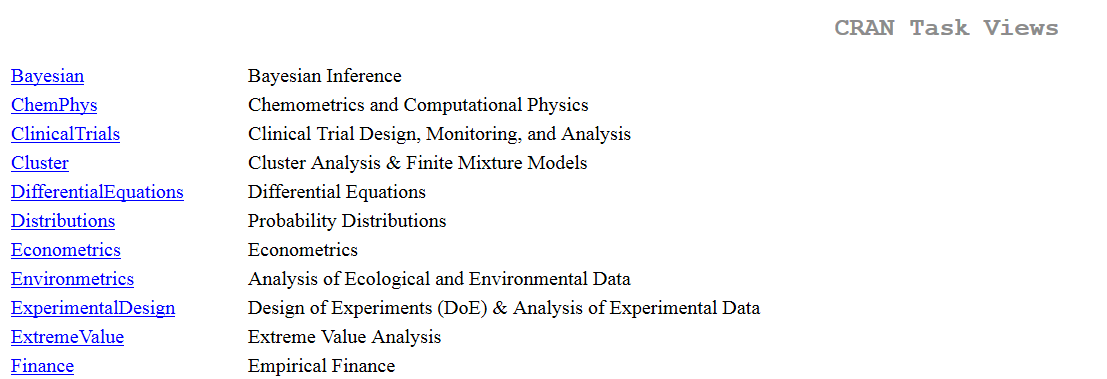
\includegraphics{figure/CRANtaskViews.PNG}
\caption{}
\end{figure}

\subsection{\texorpdfstring{Task View zu Thema
\href{https://cran.r-project.org/web/views/Graphics.html}{Graphiken}}{Task View zu Thema Graphiken}}\label{task-view-zu-thema-graphiken}

\begin{figure}[htbp]
\centering
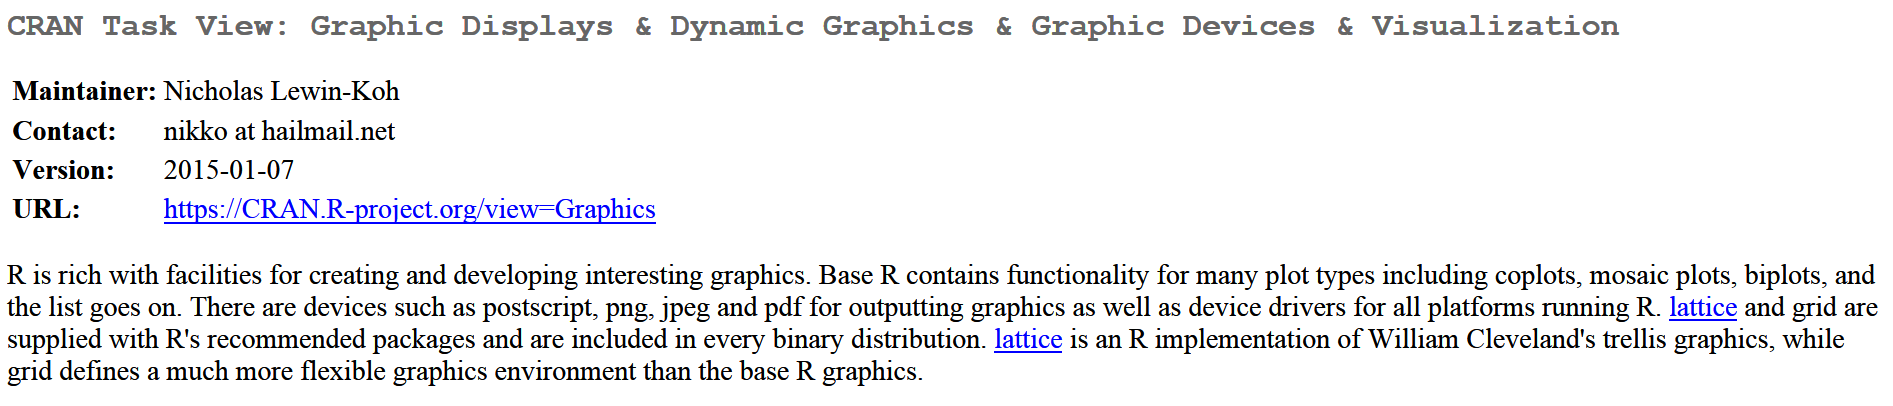
\includegraphics{figure/TaskViewGraphics.PNG}
\caption{}
\end{figure}

\subsection{Datensatz}\label{datensatz}

\begin{Shaded}
\begin{Highlighting}[]
\KeywordTok{library}\NormalTok{(mlmRev)}
\KeywordTok{data}\NormalTok{(Chem97)}
\end{Highlighting}
\end{Shaded}

\begin{itemize}
\tightlist
\item
  {[}lea{]} Local Education Authority - a factor
\item
  {[}school{]} School identifier - a factor
\item
  {[}student{]} Student identifier - a factor
\item
  {[}score{]} Point score on A-level Chemistry in 1997
\item
  {[}gender{]} Student's gender
\item
  {[}age{]} Age in month, centred at 222 months or 18.5 years
\item
  {[}gcsescore{]} Average GCSE score of individual.
\item
  {[}gcsecnt{]} Average GCSE score of individual, centered at mean.
\end{itemize}

\subsection{Histogramm - Die Funktion
hist()}\label{histogramm---die-funktion-hist}

Wir erstellen ein Histogramm der Variable gcsescore:

\begin{Shaded}
\begin{Highlighting}[]
\NormalTok{?hist}
\end{Highlighting}
\end{Shaded}

\begin{Shaded}
\begin{Highlighting}[]
\KeywordTok{hist}\NormalTok{(Chem97$gcsescore)}
\end{Highlighting}
\end{Shaded}

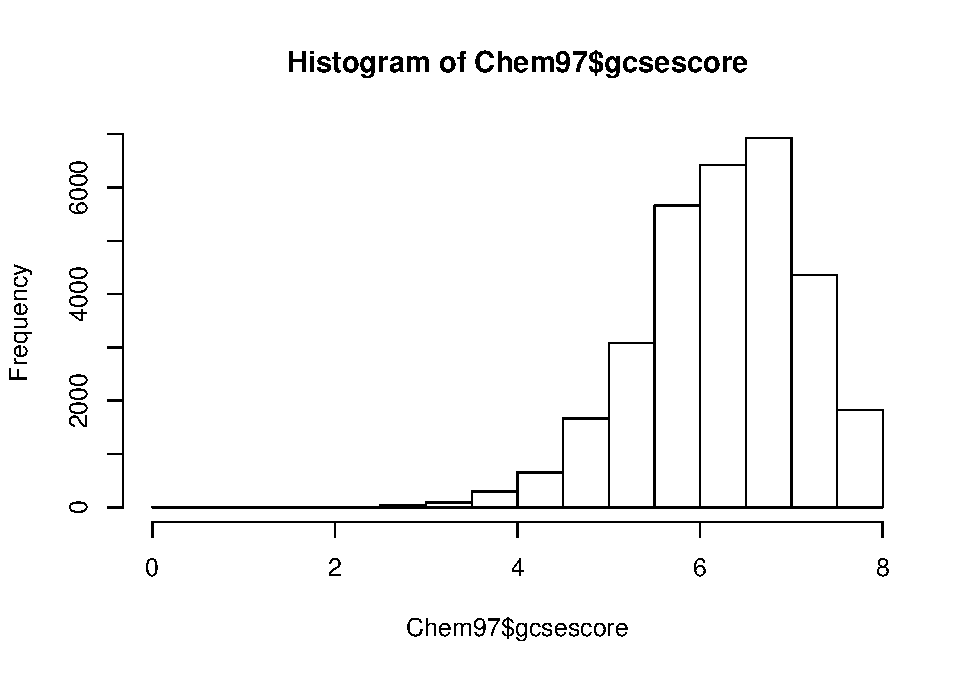
\includegraphics{Intro_Datenanalyse1_files/figure-latex/unnamed-chunk-140-1.pdf}

\subsection{Graphik speichern}\label{graphik-speichern}

\begin{itemize}
\tightlist
\item
  Mit dem button Export in Rstudio kann man die Grafik speichern.
\end{itemize}

\begin{figure}[htbp]
\centering
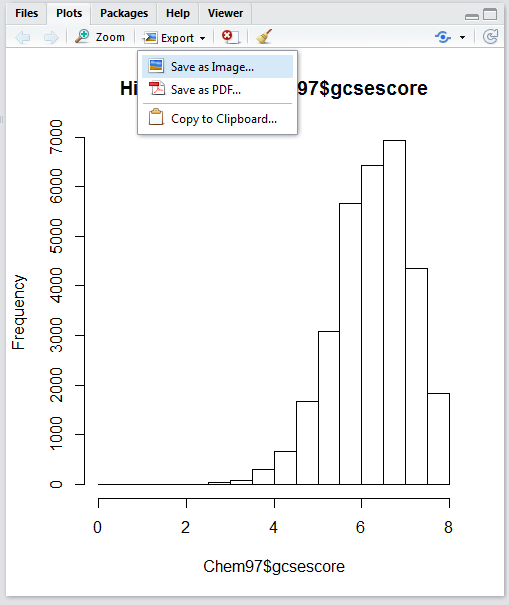
\includegraphics{figure/GraphikSpeichern.PNG}
\caption{}
\end{figure}

\subsection{Befehl um Graphik zu
speichern}\label{befehl-um-graphik-zu-speichern}

\begin{itemize}
\tightlist
\item
  Alternativ auch bspw. mit den Befehlen \texttt{png}, \texttt{pdf} oder
  \texttt{jpeg}
\end{itemize}

\begin{Shaded}
\begin{Highlighting}[]
\KeywordTok{png}\NormalTok{(}\StringTok{"Histogramm.png"}\NormalTok{)}
\KeywordTok{hist}\NormalTok{(Chem97$gcsescore)}
\KeywordTok{dev.off}\NormalTok{()}
\end{Highlighting}
\end{Shaded}

\subsection{Histogramme}\label{histogramme}

\begin{itemize}
\tightlist
\item
  Die Funktion \texttt{hist()} plottet ein Histogramm der Daten
\item
  Der Funktion muss mindestens ein Beobachtungsvektor übergeben werden
\item
  \texttt{hist()} hat noch sehr viel mehr Argumente, die alle
  (sinnvolle) default values haben
\end{itemize}

\begin{longtable}[]{@{}lll@{}}
\toprule
Argument & Bedeutung & Beispiel\tabularnewline
\midrule
\endhead
main & Überschrift & main=``Hallo Welt''\tabularnewline
xlab & x-Achsenbeschriftung & xlab=``x-Werte''\tabularnewline
ylab & y-Achsenbeschriftung & ylab=``y-Werte''\tabularnewline
col & Farbe & col=``blue''\tabularnewline
\bottomrule
\end{longtable}

\subsection{Histogramm}\label{histogramm}

\begin{Shaded}
\begin{Highlighting}[]
\KeywordTok{hist}\NormalTok{(Chem97$gcsescore,}\DataTypeTok{col=}\StringTok{"blue"}\NormalTok{,}
     \DataTypeTok{main=}\StringTok{"Hallo Welt"}\NormalTok{,}\DataTypeTok{ylab=}\StringTok{"y-Werte"}\NormalTok{, }\DataTypeTok{xlab=}\StringTok{"x-Werte"}\NormalTok{)}
\end{Highlighting}
\end{Shaded}

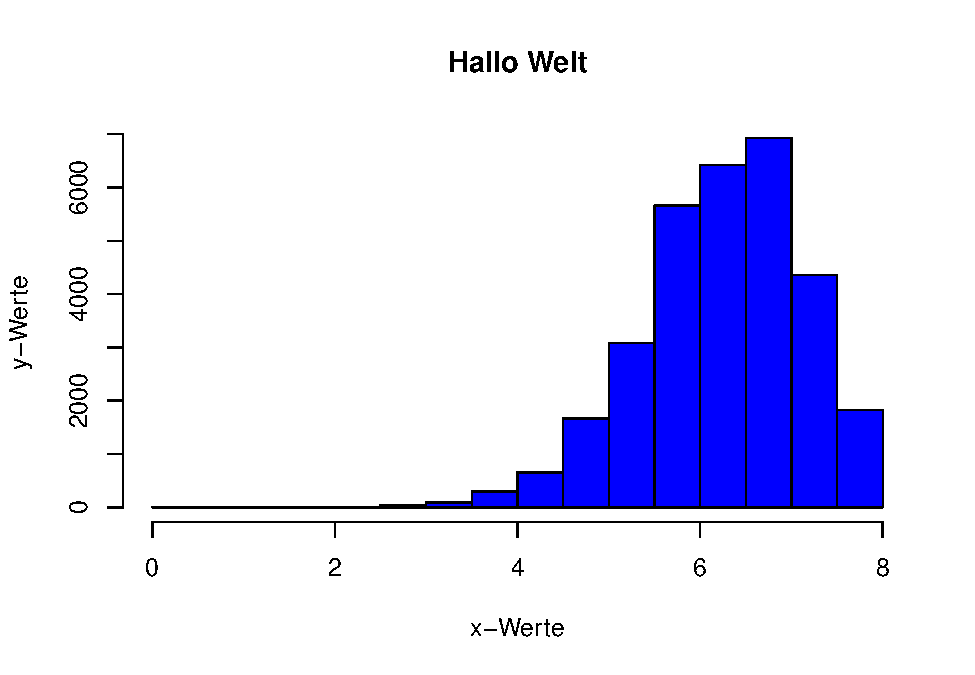
\includegraphics{Intro_Datenanalyse1_files/figure-latex/unnamed-chunk-142-1.pdf}

Weitere Argumente:

\begin{Shaded}
\begin{Highlighting}[]
\NormalTok{?plot}
\CommentTok{# oder}
\NormalTok{?par}
\end{Highlighting}
\end{Shaded}

\subsection{Barplot}\label{barplot}

\begin{itemize}
\tightlist
\item
  Die Funktion \texttt{barplot()} erzeugt aus einer Häufigkeitstabelle
  einen Barplot
\item
  Ist das übergebene Tabellen-Objekt zweidimensional wird ein bedingter
  Barplot erstellt
\end{itemize}

\begin{Shaded}
\begin{Highlighting}[]
\NormalTok{tabScore <-}\StringTok{ }\KeywordTok{table}\NormalTok{(Chem97$score)}
\end{Highlighting}
\end{Shaded}

\begin{Shaded}
\begin{Highlighting}[]
\KeywordTok{barplot}\NormalTok{(tabScore)}
\end{Highlighting}
\end{Shaded}

\subsection{Barplots und barcharts}\label{barplots-und-barcharts}

\begin{Shaded}
\begin{Highlighting}[]
\KeywordTok{barplot}\NormalTok{(tabScore)}
\end{Highlighting}
\end{Shaded}

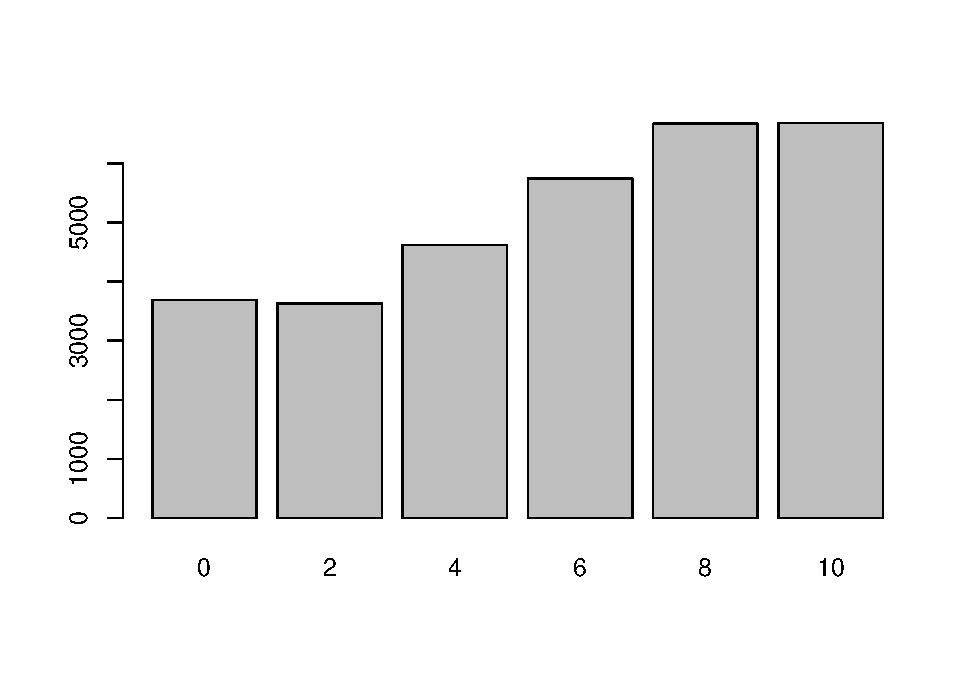
\includegraphics{Intro_Datenanalyse1_files/figure-latex/unnamed-chunk-146-1.pdf}

\subsection{Mehr Farben:}\label{mehr-farben}

\begin{Shaded}
\begin{Highlighting}[]
\KeywordTok{barplot}\NormalTok{(tabScore,}\DataTypeTok{col=}\KeywordTok{rgb}\NormalTok{(}\DecValTok{0}\NormalTok{,}\DecValTok{0}\NormalTok{,}\DecValTok{1}\NormalTok{))}
\end{Highlighting}
\end{Shaded}

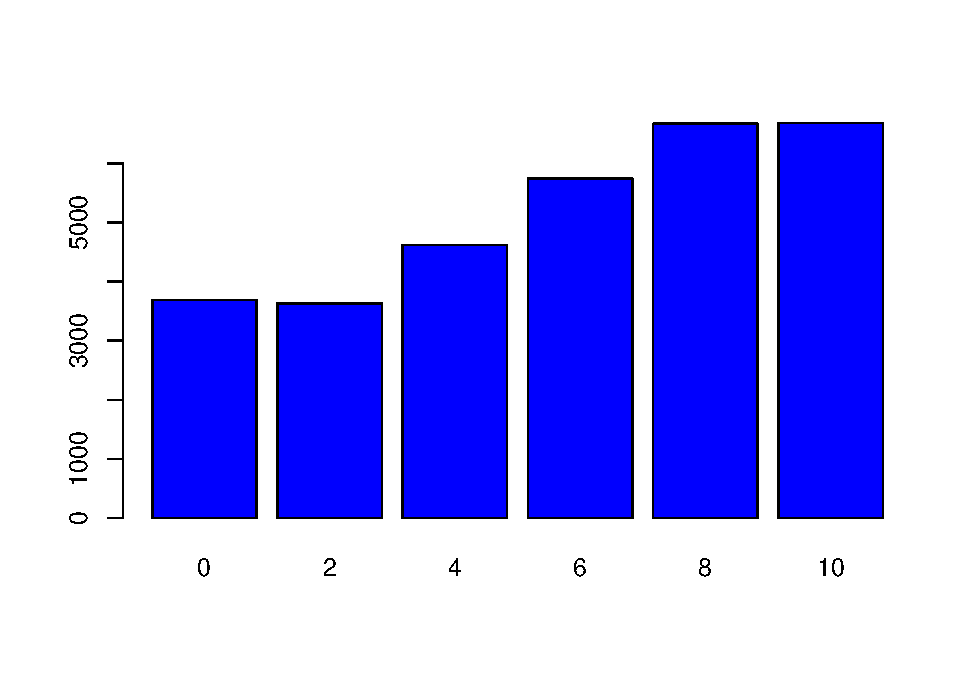
\includegraphics{Intro_Datenanalyse1_files/figure-latex/unnamed-chunk-147-1.pdf}

\subsection{Grüne Farbe}\label{grune-farbe}

\begin{Shaded}
\begin{Highlighting}[]
\KeywordTok{barplot}\NormalTok{(tabScore,}\DataTypeTok{col=}\KeywordTok{rgb}\NormalTok{(}\DecValTok{0}\NormalTok{,}\DecValTok{1}\NormalTok{,}\DecValTok{0}\NormalTok{))}
\end{Highlighting}
\end{Shaded}

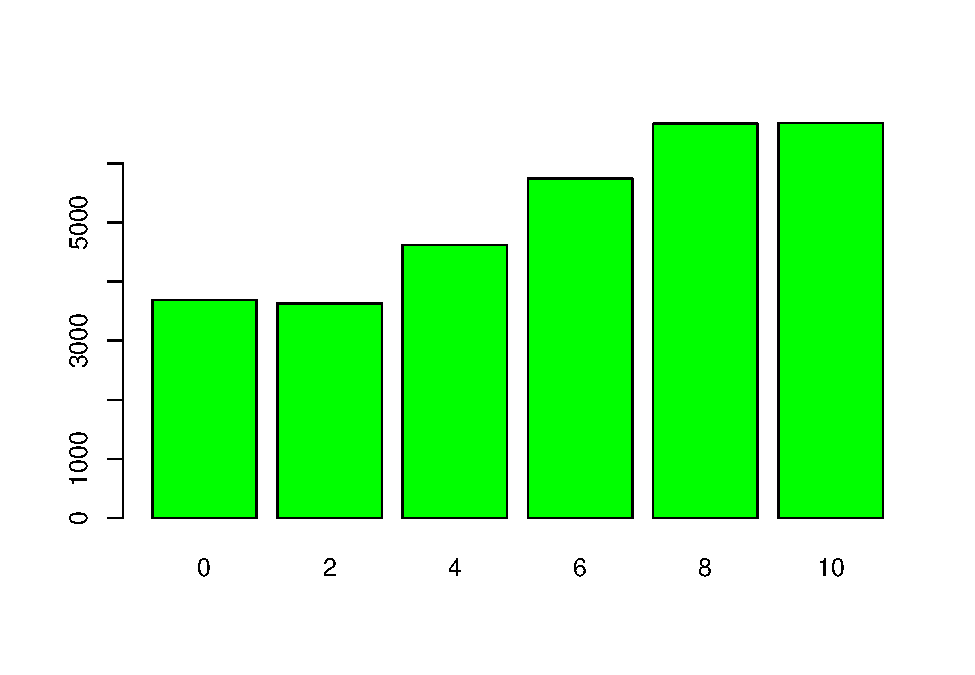
\includegraphics{Intro_Datenanalyse1_files/figure-latex/unnamed-chunk-148-1.pdf}

\subsection{Rote Farbe}\label{rote-farbe}

\begin{Shaded}
\begin{Highlighting}[]
\KeywordTok{barplot}\NormalTok{(tabScore,}\DataTypeTok{col=}\KeywordTok{rgb}\NormalTok{(}\DecValTok{1}\NormalTok{,}\DecValTok{0}\NormalTok{,}\DecValTok{0}\NormalTok{))}
\end{Highlighting}
\end{Shaded}

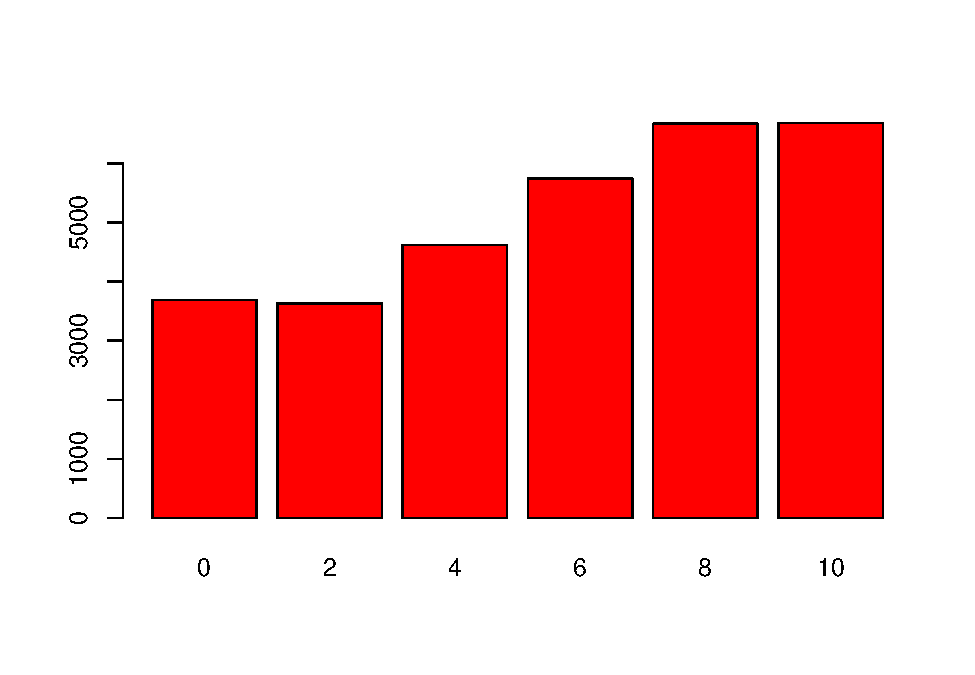
\includegraphics{Intro_Datenanalyse1_files/figure-latex/unnamed-chunk-149-1.pdf}

\subsection{Transparent}\label{transparent}

\begin{Shaded}
\begin{Highlighting}[]
\KeywordTok{barplot}\NormalTok{(tabScore,}\DataTypeTok{col=}\KeywordTok{rgb}\NormalTok{(}\DecValTok{1}\NormalTok{,}\DecValTok{0}\NormalTok{,}\DecValTok{0}\NormalTok{,.}\DecValTok{3}\NormalTok{))}
\end{Highlighting}
\end{Shaded}

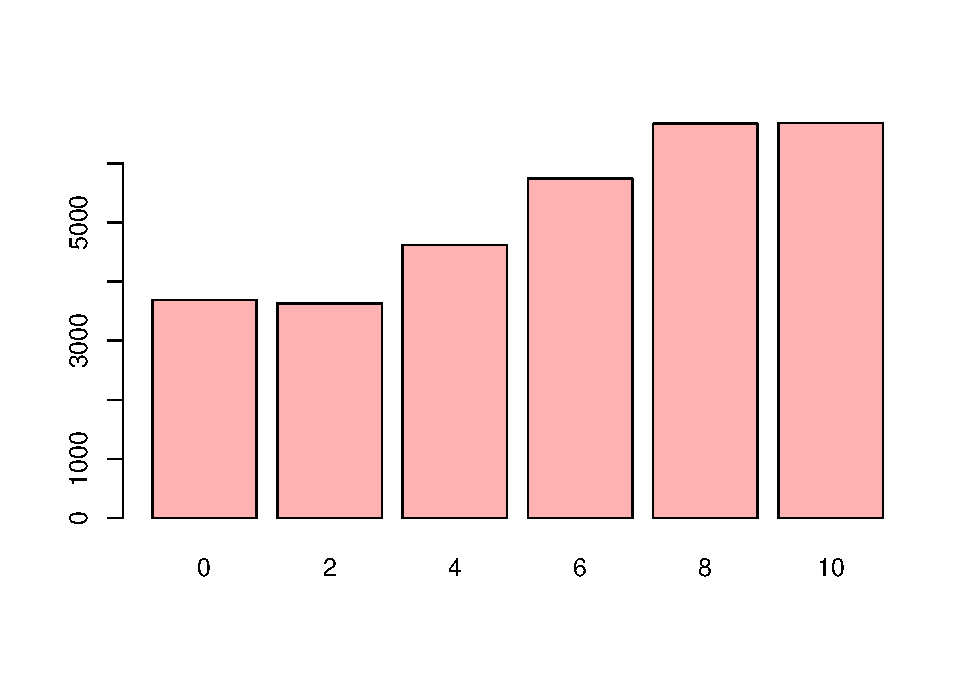
\includegraphics{Intro_Datenanalyse1_files/figure-latex/unnamed-chunk-150-1.pdf}

\subsection{Boxplot}\label{boxplot}

\begin{itemize}
\tightlist
\item
  Einen einfachen Boxplot erstellt man mit \texttt{boxplot()}
\item
  Auch \texttt{boxplot()} muss mindestens ein Beobachtungsvektor
  übergeben werden
\end{itemize}

\begin{Shaded}
\begin{Highlighting}[]
\NormalTok{?boxplot}
\end{Highlighting}
\end{Shaded}

\subsection{Horizontaler Boxplot}\label{horizontaler-boxplot}

\begin{Shaded}
\begin{Highlighting}[]
\KeywordTok{boxplot}\NormalTok{(Chem97$gcsescore,}
\DataTypeTok{horizontal=}\OtherTok{TRUE}\NormalTok{)}
\end{Highlighting}
\end{Shaded}

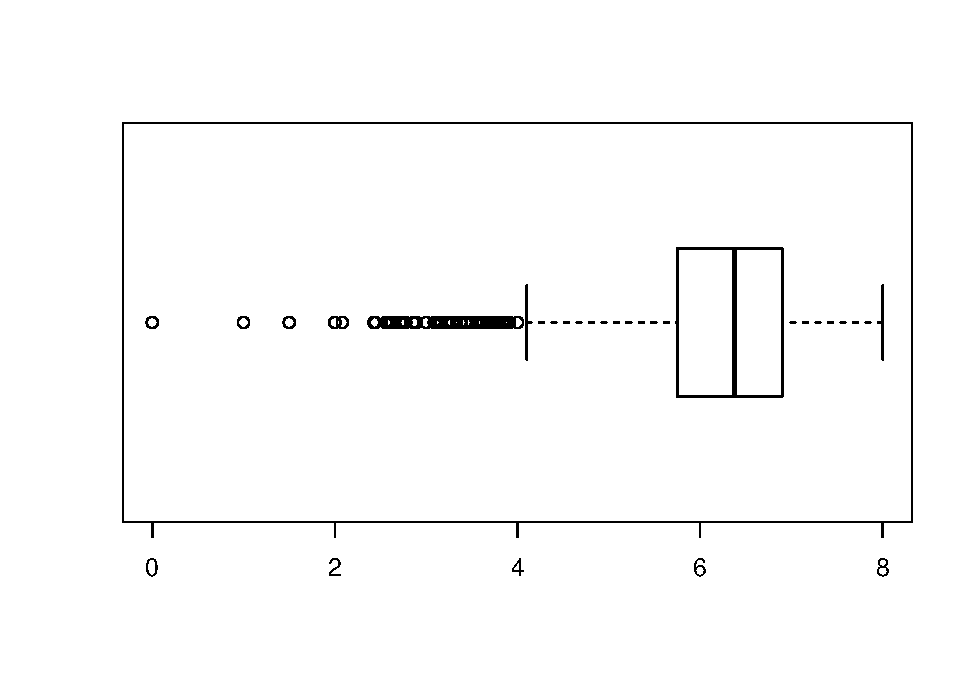
\includegraphics{Intro_Datenanalyse1_files/figure-latex/unnamed-chunk-152-1.pdf}

\begin{itemize}
\tightlist
\item
  \href{http://edoc.hu-berlin.de/dissertationen/gruenwald-andreas-2005-01-17/HTML/chapter2.html}{Erklärung
  zu Boxplots}
\end{itemize}

\subsection{Gruppierte Boxplots}\label{gruppierte-boxplots}

\begin{itemize}
\tightlist
\item
  Ein sehr einfacher Weg, einen ersten Eindruck über bedingte
  Verteilungen zu bekommen ist über sog. Gruppierte notched Boxplots
\item
  Dazu muss der Funktion \texttt{boxplot()} ein sog. Formel-Objekt
  übergeben werden
\item
  Die bedingende Variable steht dabei auf der rechten Seite einer Tilde
\end{itemize}

\subsection{Beispiel grupierter
Boxplot}\label{beispiel-grupierter-boxplot}

\begin{Shaded}
\begin{Highlighting}[]
\KeywordTok{boxplot}\NormalTok{(Chem97$gcsescore~Chem97$gender)}
\end{Highlighting}
\end{Shaded}

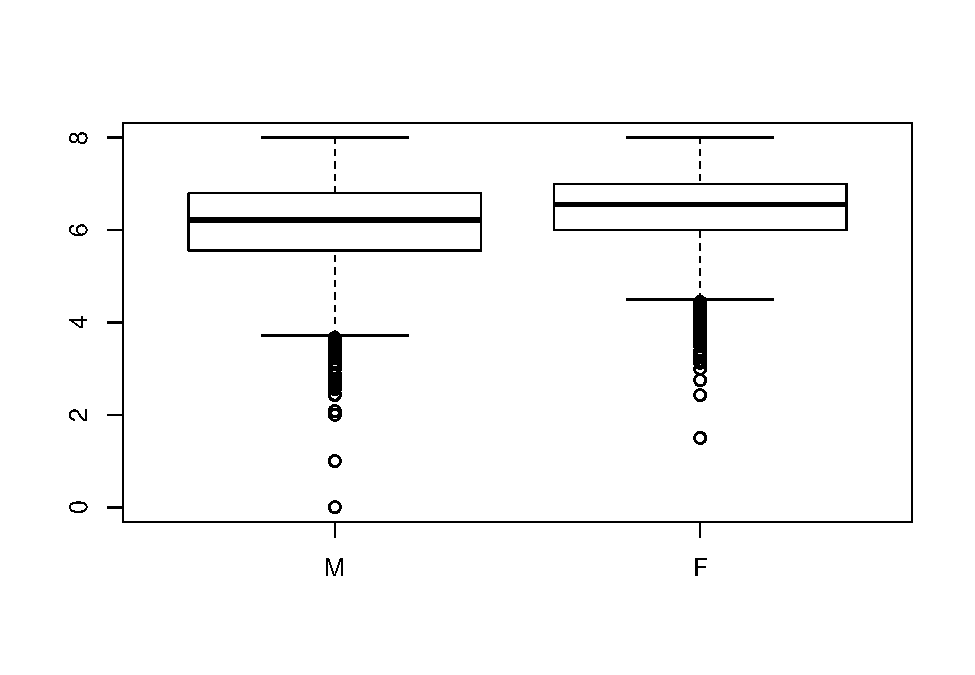
\includegraphics{Intro_Datenanalyse1_files/figure-latex/unnamed-chunk-153-1.pdf}

\subsection{Alternativen zu Boxplot}\label{alternativen-zu-boxplot}

Violinplot

\begin{itemize}
\tightlist
\item
  Baut auf Boxplot auf
\item
  Zusätzlich Informationen über Dichte der Daten
\item
  Dichte wird über Kernel Methode berechnet.
\item
  weißer Punkt - Median
\item
  Je weiter die Ausdehnung, desto größer ist die Dichte an dieser
  Stelle.
\end{itemize}

\begin{Shaded}
\begin{Highlighting}[]
\CommentTok{# Beispieldaten erzeugen}
\NormalTok{x <-}\StringTok{ }\KeywordTok{rnorm}\NormalTok{(}\DecValTok{100}\NormalTok{)}
\NormalTok{y <-}\StringTok{ }\KeywordTok{rnorm}\NormalTok{(}\DecValTok{100}\NormalTok{)}
\end{Highlighting}
\end{Shaded}

\subsection{\texorpdfstring{Die Bibliothek
\texttt{vioplot}}{Die Bibliothek vioplot}}\label{die-bibliothek-vioplot}

\begin{Shaded}
\begin{Highlighting}[]
\KeywordTok{library}\NormalTok{(vioplot)}
\KeywordTok{plot}\NormalTok{(x, y, }\DataTypeTok{xlim=}\KeywordTok{c}\NormalTok{(-}\DecValTok{5}\NormalTok{,}\DecValTok{5}\NormalTok{), }\DataTypeTok{ylim=}\KeywordTok{c}\NormalTok{(-}\DecValTok{5}\NormalTok{,}\DecValTok{5}\NormalTok{))}
\KeywordTok{vioplot}\NormalTok{(x, }\DataTypeTok{col=}\StringTok{"tomato"}\NormalTok{, }\DataTypeTok{horizontal=}\OtherTok{TRUE}\NormalTok{, }\DataTypeTok{at=}\NormalTok{-}\DecValTok{4}\NormalTok{, }
        \DataTypeTok{add=}\OtherTok{TRUE}\NormalTok{,}\DataTypeTok{lty=}\DecValTok{2}\NormalTok{, }\DataTypeTok{rectCol=}\StringTok{"gray"}\NormalTok{)}
\KeywordTok{vioplot}\NormalTok{(y, }\DataTypeTok{col=}\StringTok{"cyan"}\NormalTok{, }\DataTypeTok{horizontal=}\OtherTok{FALSE}\NormalTok{, }\DataTypeTok{at=}\NormalTok{-}\DecValTok{4}\NormalTok{, }
        \DataTypeTok{add=}\OtherTok{TRUE}\NormalTok{,}\DataTypeTok{lty=}\DecValTok{2}\NormalTok{)}
\end{Highlighting}
\end{Shaded}

\subsection{\texorpdfstring{\texttt{vioplot} - Das
Ergebnis}{vioplot - Das Ergebnis}}\label{vioplot---das-ergebnis}

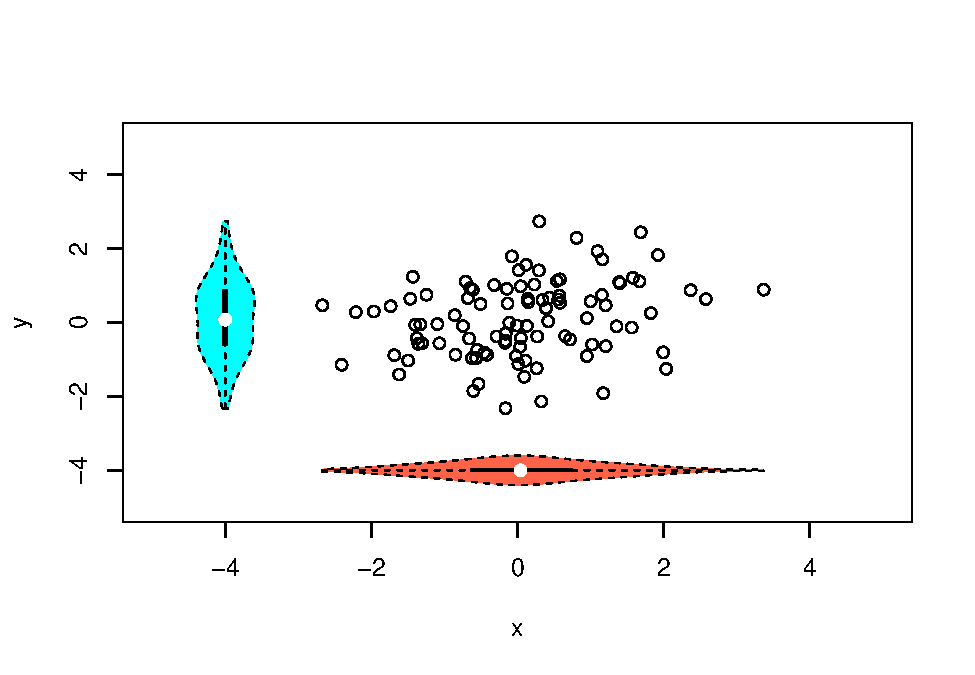
\includegraphics{Intro_Datenanalyse1_files/figure-latex/unnamed-chunk-156-1.pdf}

\subsection{Alternativen zum Boxplot}\label{alternativen-zum-boxplot}

\begin{Shaded}
\begin{Highlighting}[]
\KeywordTok{library}\NormalTok{(beanplot)}
\KeywordTok{par}\NormalTok{(}\DataTypeTok{mfrow =} \KeywordTok{c}\NormalTok{(}\DecValTok{1}\NormalTok{,}\DecValTok{2}\NormalTok{))}
\KeywordTok{boxplot}\NormalTok{(count~spray,}\DataTypeTok{data=}\NormalTok{InsectSprays,}\DataTypeTok{col=}\StringTok{"blue"}\NormalTok{)}
\KeywordTok{beanplot}\NormalTok{(count~spray,}\DataTypeTok{data=}\NormalTok{InsectSprays,}\DataTypeTok{col=}\StringTok{"orange"}\NormalTok{)}
\end{Highlighting}
\end{Shaded}

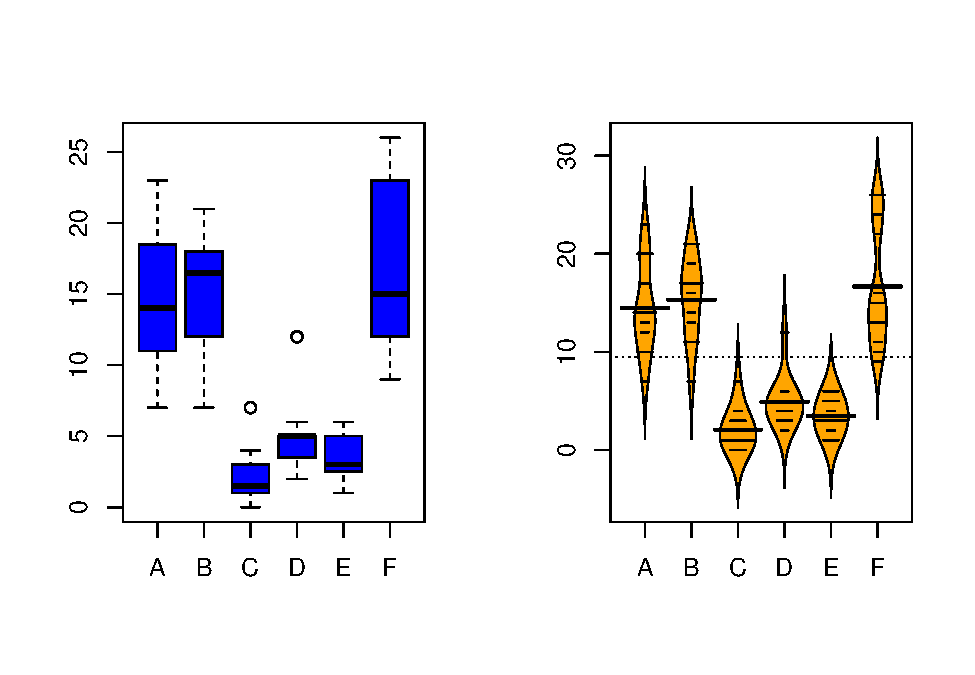
\includegraphics{Intro_Datenanalyse1_files/figure-latex/unnamed-chunk-157-1.pdf}

\section{Grafiken für bedingte, bi- und multivariate
Verteilungen}\label{grafiken-fur-bedingte-bi--und-multivariate-verteilungen}

\subsection{Scatterplots}\label{scatterplots}

\begin{itemize}
\tightlist
\item
  Ein einfacher two-way scatterplot kann mit der Funktion plot()
  erstellt werden
\item
  plot() muss mindestens ein x und ein y Beobachtungsvektor übergeben
  werden
\item
  Um die Farbe der Plot-Symbole anzupassen gibt es die Option col (Farbe
  als character oder numerisch)
\item
  Die Plot-Symbole selbst können mit pch\} (plotting character)
  angepasst werden (character oder numerisch)
\item
  Die Achenbeschriftungen (labels) werden mit xlab und ylab definiert
\end{itemize}

\subsection{Aufgabe - einfache
Grafiken}\label{aufgabe---einfache-grafiken}

\begin{itemize}
\tightlist
\item
  Laden Sie den Datensatz \texttt{VADeaths} und erzeugen Sie den
  folgenden plot:
\end{itemize}

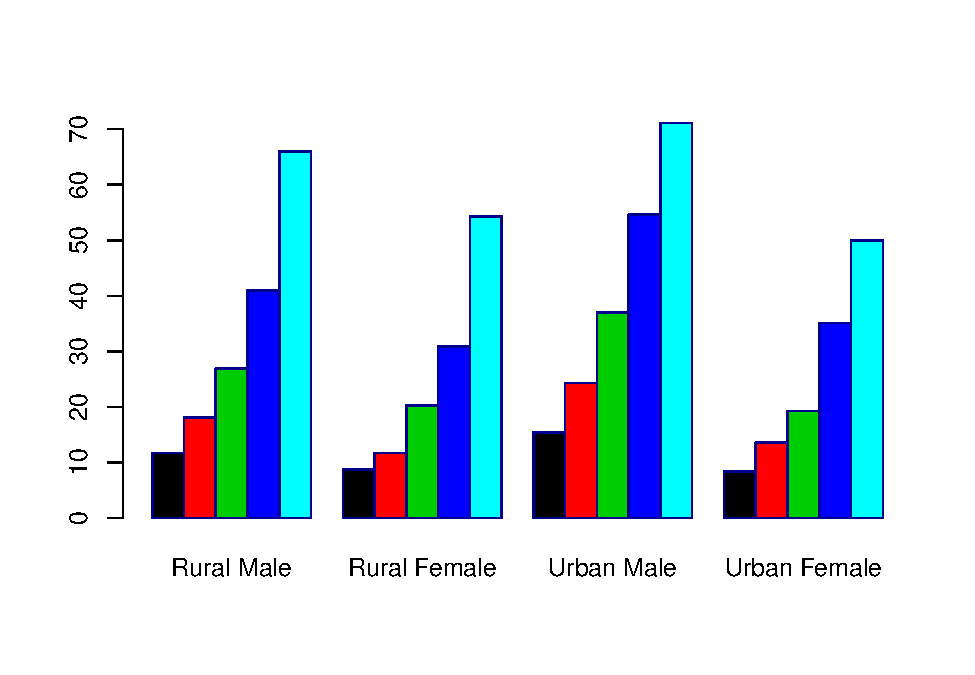
\includegraphics{Intro_Datenanalyse1_files/figure-latex/unnamed-chunk-158-1.pdf}

\href{https://github.com/Japhilko/IntroR/blob/master/2017/README.md}{Zurück
zur Gliederung.}

\section{Zusammenhang}\label{zusammenhang}

\subsection{Edgar Anderson's Iris
Daten}\label{edgar-andersons-iris-daten}

\begin{Shaded}
\begin{Highlighting}[]
\KeywordTok{data}\NormalTok{(iris)}
\KeywordTok{head}\NormalTok{(iris)}
\end{Highlighting}
\end{Shaded}

\begin{verbatim}
##   Sepal.Length Sepal.Width Petal.Length Petal.Width Species
## 1          5.1         3.5          1.4         0.2  setosa
## 2          4.9         3.0          1.4         0.2  setosa
## 3          4.7         3.2          1.3         0.2  setosa
## 4          4.6         3.1          1.5         0.2  setosa
## 5          5.0         3.6          1.4         0.2  setosa
## 6          5.4         3.9          1.7         0.4  setosa
\end{verbatim}

petal length and width - Blütenblatt Länge und Breite

sepal length and width - Kelchblatt Länge und Breite

\begin{itemize}
\tightlist
\item
  \href{https://en.wikipedia.org/wiki/Iris_flower_data_set}{Wikipedia
  Artikel zum IRIS Datensatz}
\end{itemize}

\subsection{Zusammenhang zwischen stetigen
Variablen}\label{zusammenhang-zwischen-stetigen-variablen}

\begin{Shaded}
\begin{Highlighting}[]
\CommentTok{# Pearson Korrelationskoeffizient}
\KeywordTok{cor}\NormalTok{(iris$Sepal.Length,iris$Petal.Length)}
\end{Highlighting}
\end{Shaded}

\begin{verbatim}
## [1] 0.8717538
\end{verbatim}

\begin{itemize}
\tightlist
\item
  Korrelation zwischen Länge Kelchblatt und Blütenblatt 0,87
\item
  Der Pearson'sche Korrelationskoeffizient ist die default methode in
  \texttt{cor()}.
\end{itemize}

\subsection{Zusammenhang zwischen mehreren
Variablen}\label{zusammenhang-zwischen-mehreren-variablen}

\begin{Shaded}
\begin{Highlighting}[]
\KeywordTok{pairs}\NormalTok{(iris[,}\DecValTok{1}\NormalTok{:}\DecValTok{4}\NormalTok{])}
\end{Highlighting}
\end{Shaded}

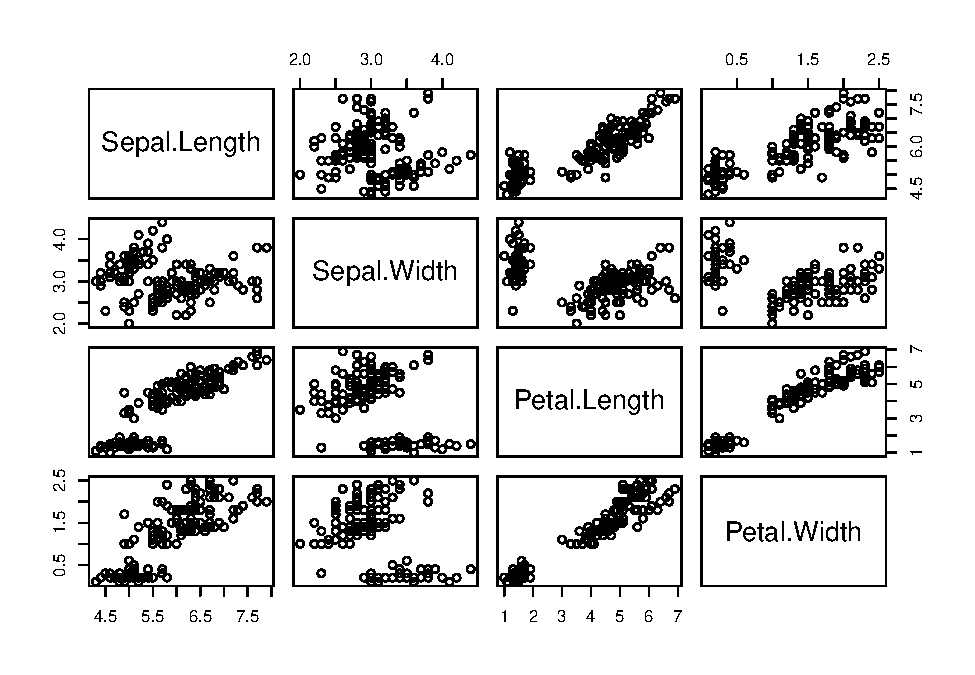
\includegraphics{Intro_Datenanalyse1_files/figure-latex/unnamed-chunk-162-1.pdf}

\subsection{Zusammenhang zwischen mehreren
Variablen}\label{zusammenhang-zwischen-mehreren-variablen-1}

\begin{Shaded}
\begin{Highlighting}[]
\KeywordTok{library}\NormalTok{(}\StringTok{"psych"}\NormalTok{)}
\KeywordTok{pairs.panels}\NormalTok{(iris[}\DecValTok{1}\NormalTok{:}\DecValTok{4}\NormalTok{],}\DataTypeTok{bg=}\KeywordTok{c}\NormalTok{(}\StringTok{"red"}\NormalTok{,}\StringTok{"yellow"}\NormalTok{,}\StringTok{"blue"}\NormalTok{)}
\NormalTok{[iris$Species],}\DataTypeTok{pch=}\DecValTok{21}\NormalTok{,}\DataTypeTok{main=}\StringTok{""}\NormalTok{)}
\end{Highlighting}
\end{Shaded}

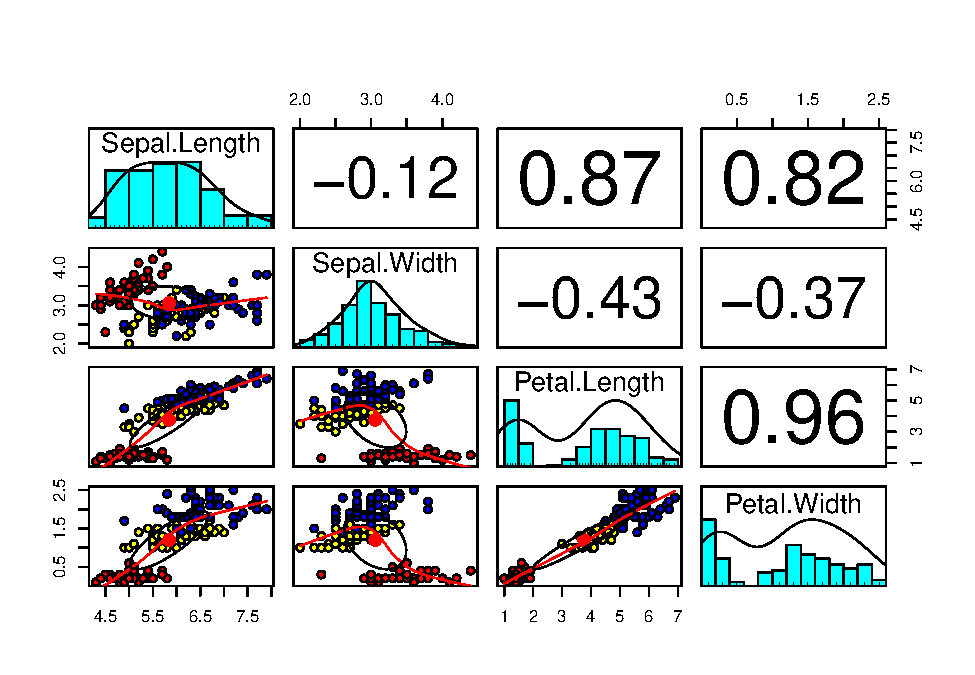
\includegraphics{Intro_Datenanalyse1_files/figure-latex/unnamed-chunk-163-1.pdf}

\subsection{Verschiedene
Korrelationskoeffizienten}\label{verschiedene-korrelationskoeffizienten}

\begin{Shaded}
\begin{Highlighting}[]
\CommentTok{# Pearson Korrelationskoeffizient}
\KeywordTok{cor}\NormalTok{(iris[,}\DecValTok{1}\NormalTok{:}\DecValTok{4}\NormalTok{]) }
\end{Highlighting}
\end{Shaded}

\begin{verbatim}
##              Sepal.Length Sepal.Width Petal.Length Petal.Width
## Sepal.Length    1.0000000  -0.1175698    0.8717538   0.8179411
## Sepal.Width    -0.1175698   1.0000000   -0.4284401  -0.3661259
## Petal.Length    0.8717538  -0.4284401    1.0000000   0.9628654
## Petal.Width     0.8179411  -0.3661259    0.9628654   1.0000000
\end{verbatim}

\begin{Shaded}
\begin{Highlighting}[]
\CommentTok{# Kendall's tau (Rangkorrelation)}
\KeywordTok{cor}\NormalTok{(iris[,}\DecValTok{1}\NormalTok{:}\DecValTok{4}\NormalTok{], }\DataTypeTok{method =} \StringTok{"kendall"}\NormalTok{) }
\end{Highlighting}
\end{Shaded}

\begin{verbatim}
##              Sepal.Length Sepal.Width Petal.Length Petal.Width
## Sepal.Length   1.00000000 -0.07699679    0.7185159   0.6553086
## Sepal.Width   -0.07699679  1.00000000   -0.1859944  -0.1571257
## Petal.Length   0.71851593 -0.18599442    1.0000000   0.8068907
## Petal.Width    0.65530856 -0.15712566    0.8068907   1.0000000
\end{verbatim}

\begin{Shaded}
\begin{Highlighting}[]
\CommentTok{# Spearman's rho (Rangkorrelation)}
\KeywordTok{cor}\NormalTok{(iris[,}\DecValTok{1}\NormalTok{:}\DecValTok{4}\NormalTok{], }\DataTypeTok{method =} \StringTok{"spearman"}\NormalTok{) }
\end{Highlighting}
\end{Shaded}

\begin{verbatim}
##              Sepal.Length Sepal.Width Petal.Length Petal.Width
## Sepal.Length    1.0000000  -0.1667777    0.8818981   0.8342888
## Sepal.Width    -0.1667777   1.0000000   -0.3096351  -0.2890317
## Petal.Length    0.8818981  -0.3096351    1.0000000   0.9376668
## Petal.Width     0.8342888  -0.2890317    0.9376668   1.0000000
\end{verbatim}

\subsection{Zusammenhang zwischen kategorialen
Variablen}\label{zusammenhang-zwischen-kategorialen-variablen}

\begin{itemize}
\tightlist
\item
  chisq.test() testet, ob zwei kategoriale Merkmale stochastisch
  unabhängig sind.
\item
  Getestet wird gegen die Nullhypothese der Gleichverteilung
\end{itemize}

\subsection{Levelplot}\label{levelplot}

\begin{Shaded}
\begin{Highlighting}[]
\KeywordTok{library}\NormalTok{(}\StringTok{"lattice"}\NormalTok{)}
\KeywordTok{library}\NormalTok{(}\StringTok{"AER"}\NormalTok{)}
\KeywordTok{data}\NormalTok{(BankWages)}
\KeywordTok{levelplot}\NormalTok{(}\KeywordTok{table}\NormalTok{(BankWages$education,BankWages$job))}
\end{Highlighting}
\end{Shaded}

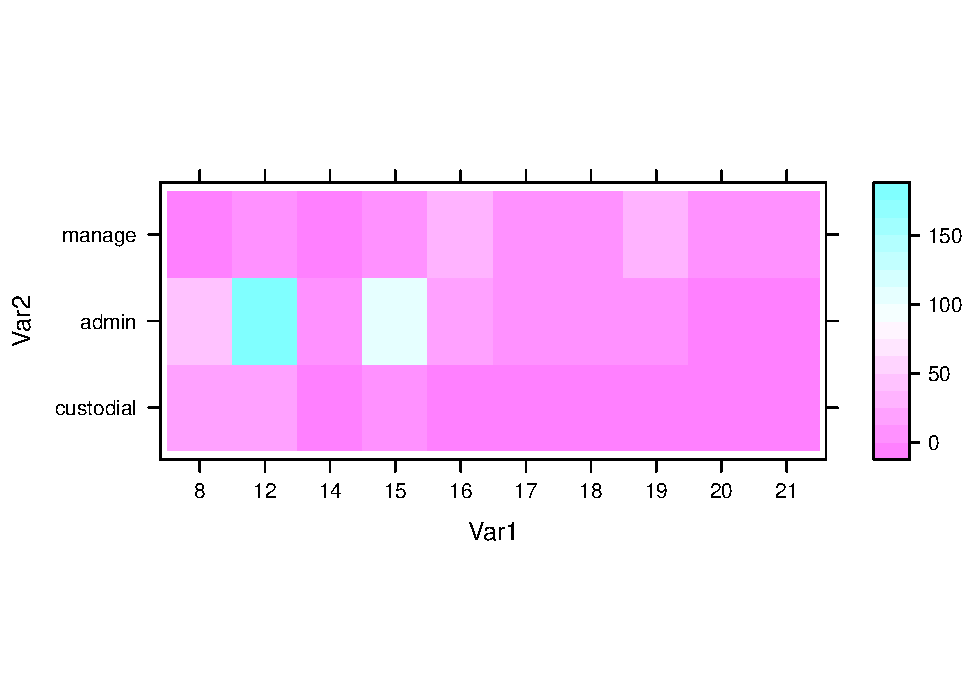
\includegraphics{Intro_Datenanalyse1_files/figure-latex/unnamed-chunk-167-1.pdf}

\subsection{Visualisierung von Zusammenhängen zwischen kategorialen
Variablen}\label{visualisierung-von-zusammenhangen-zwischen-kategorialen-variablen}

\begin{Shaded}
\begin{Highlighting}[]
\KeywordTok{mosaicplot}\NormalTok{(~}\StringTok{ }\NormalTok{Sex +}\StringTok{ }\NormalTok{Age +}\StringTok{ }\NormalTok{Survived, }
           \DataTypeTok{data =} \NormalTok{Titanic, }\DataTypeTok{color =} \OtherTok{TRUE}\NormalTok{)}
\end{Highlighting}
\end{Shaded}

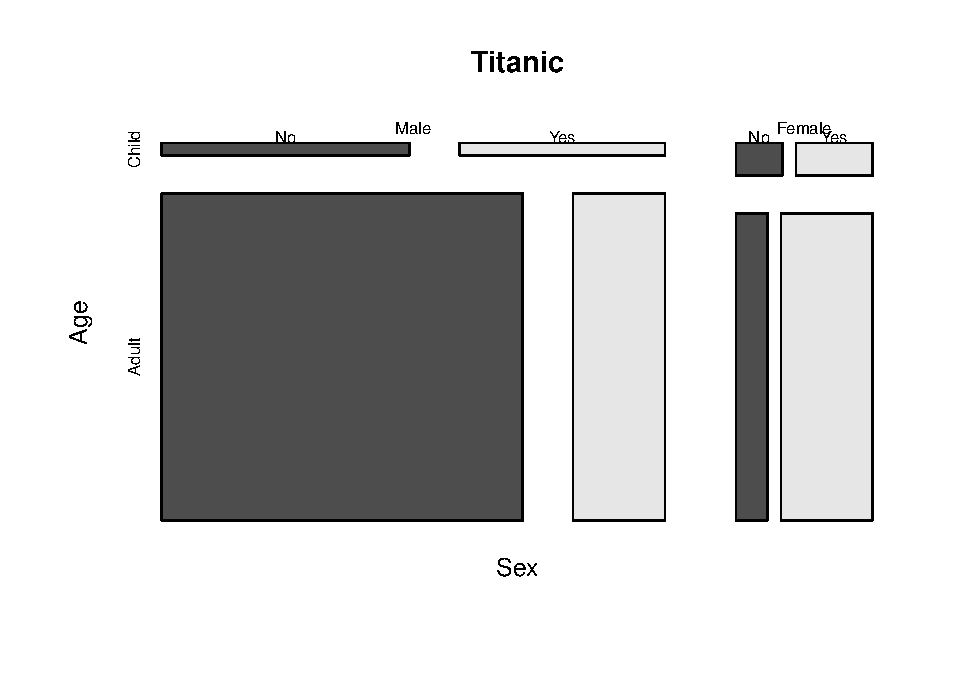
\includegraphics{Intro_Datenanalyse1_files/figure-latex/unnamed-chunk-168-1.pdf}

\subsection{Shading}\label{shading}

Flächen werden entsprechend der Residuen eingefärbt:

\begin{Shaded}
\begin{Highlighting}[]
\KeywordTok{mosaicplot}\NormalTok{(~}\StringTok{ }\NormalTok{Sex +}\StringTok{ }\NormalTok{Age +}\StringTok{ }\NormalTok{Survived, }
           \DataTypeTok{data =} \NormalTok{Titanic, }\DataTypeTok{shade =} \OtherTok{TRUE}\NormalTok{)}
\end{Highlighting}
\end{Shaded}

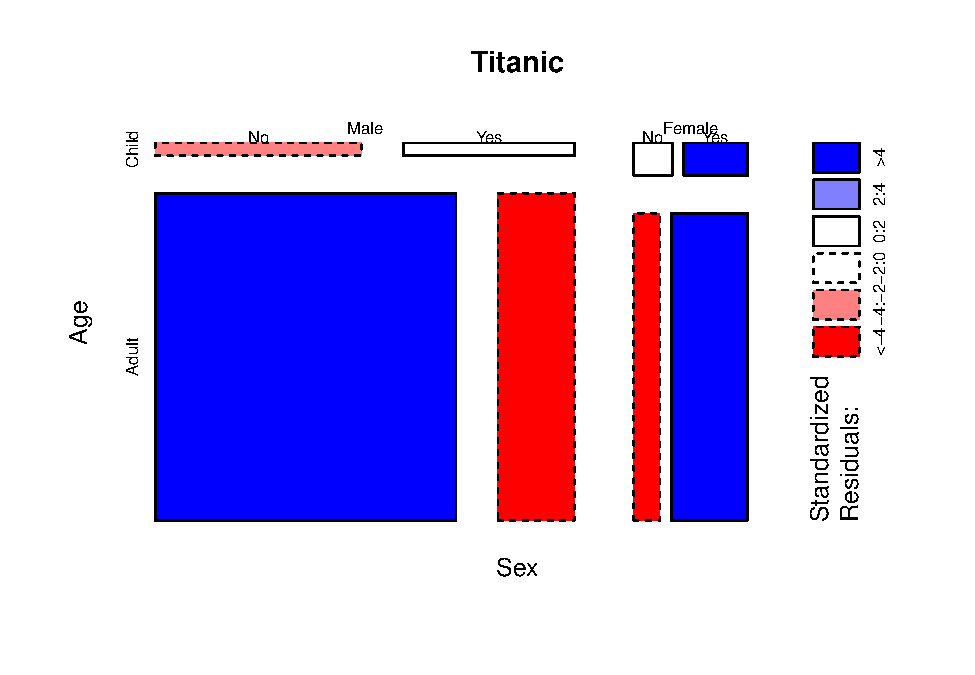
\includegraphics{Intro_Datenanalyse1_files/figure-latex/unnamed-chunk-169-1.pdf}

\subsection{Literatur zu
Zusammenhangsmaßen}\label{literatur-zu-zusammenhangsmaen}

\begin{itemize}
\tightlist
\item
  Methodensammlung mit R
\item
  Beispiele zu Zusammenhangsmaßen
\item
  Umsetzung in R
\end{itemize}

Sachs -
\href{https://books.google.de/books/about/Angewandte_Statistik.html?id=S-zXmAEACAAJ\&redir_esc=y}{Angewandte
Statistik mit R}

\section{Das lattice Paket}\label{das-lattice-paket}

\subsection{Das lattice-Paket}\label{das-lattice-paket-1}

\begin{quote}
It is designed to meet most typical graphics needs with minimal tuning,
but can also be easily extended to handle most nonstandard requirements.
\end{quote}

\url{http://stat.ethz.ch/R-manual/R-devel/library/lattice/html/Lattice.html}

\subsection{Histogramm mit Lattice}\label{histogramm-mit-lattice}

\begin{Shaded}
\begin{Highlighting}[]
\KeywordTok{library}\NormalTok{(}\StringTok{"lattice"}\NormalTok{);}\KeywordTok{library}\NormalTok{(}\StringTok{"mlmRev"}\NormalTok{)}
\KeywordTok{data}\NormalTok{(Chem97)}
\KeywordTok{histogram}\NormalTok{(~}\StringTok{ }\NormalTok{gcsescore, }\DataTypeTok{data =} \NormalTok{Chem97)}
\end{Highlighting}
\end{Shaded}

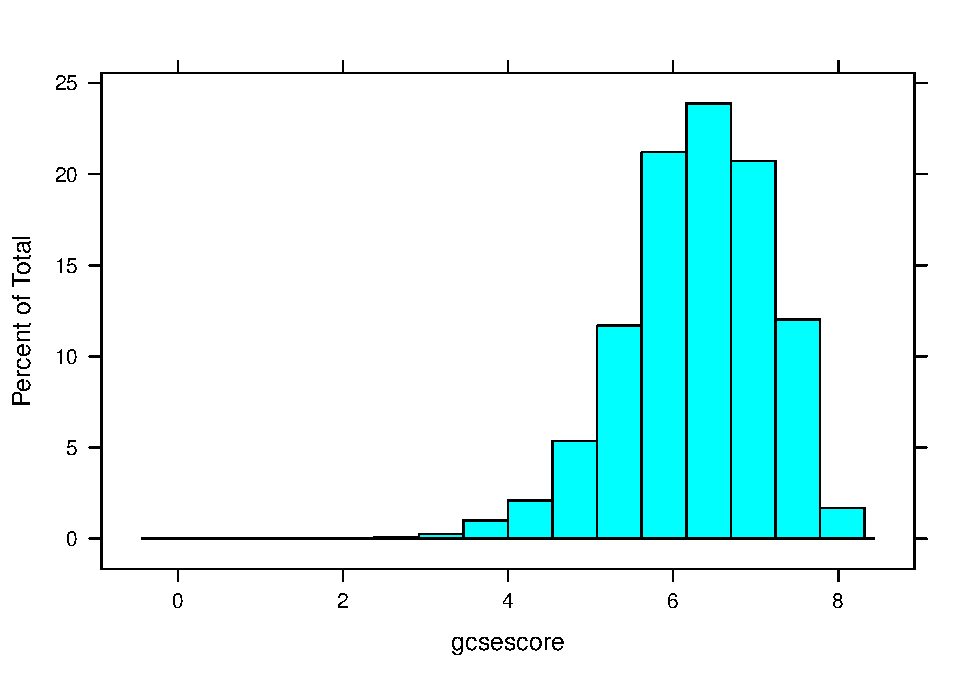
\includegraphics{Intro_Datenanalyse1_files/figure-latex/unnamed-chunk-171-1.pdf}

\subsection{Histogramm mit Lattice}\label{histogramm-mit-lattice-1}

\begin{Shaded}
\begin{Highlighting}[]
  \KeywordTok{histogram}\NormalTok{(~}\StringTok{ }\NormalTok{gcsescore |}\StringTok{ }\KeywordTok{factor}\NormalTok{(score),}\DataTypeTok{data =} \NormalTok{Chem97)}
\end{Highlighting}
\end{Shaded}

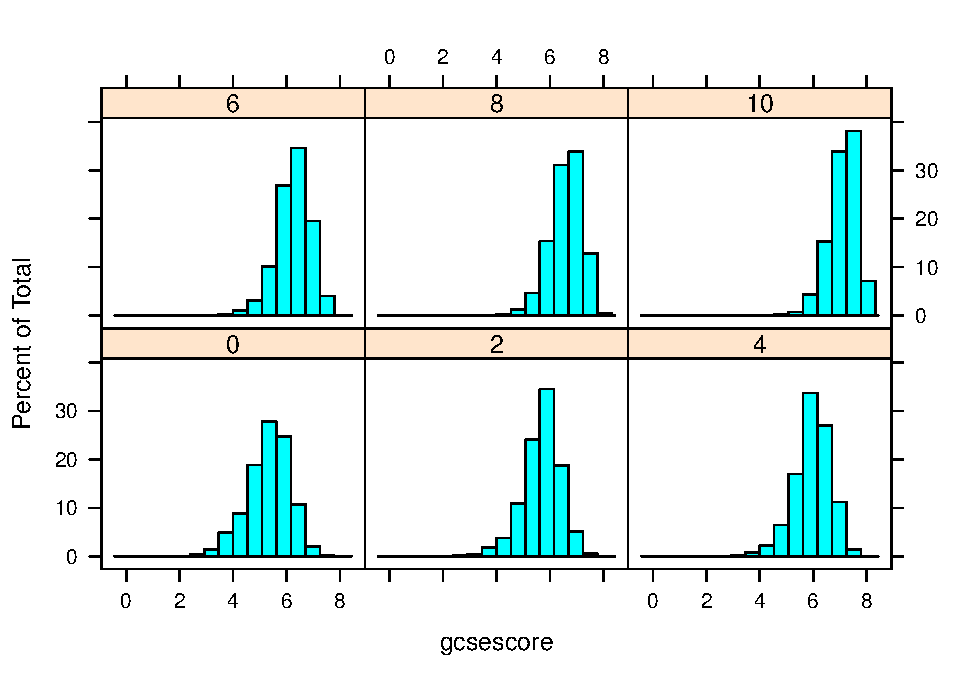
\includegraphics{Intro_Datenanalyse1_files/figure-latex/unnamed-chunk-172-1.pdf}

\subsection{Die Dichte mit Lattice
zeichnen}\label{die-dichte-mit-lattice-zeichnen}

\begin{Shaded}
\begin{Highlighting}[]
\KeywordTok{densityplot}\NormalTok{(~}\StringTok{ }\NormalTok{gcsescore |}\StringTok{ }\KeywordTok{factor}\NormalTok{(score), Chem97, }
    \DataTypeTok{groups=}\NormalTok{gender,}\DataTypeTok{plot.points=}\OtherTok{FALSE}\NormalTok{,}\DataTypeTok{auto.key=}\OtherTok{TRUE}\NormalTok{)}
\end{Highlighting}
\end{Shaded}

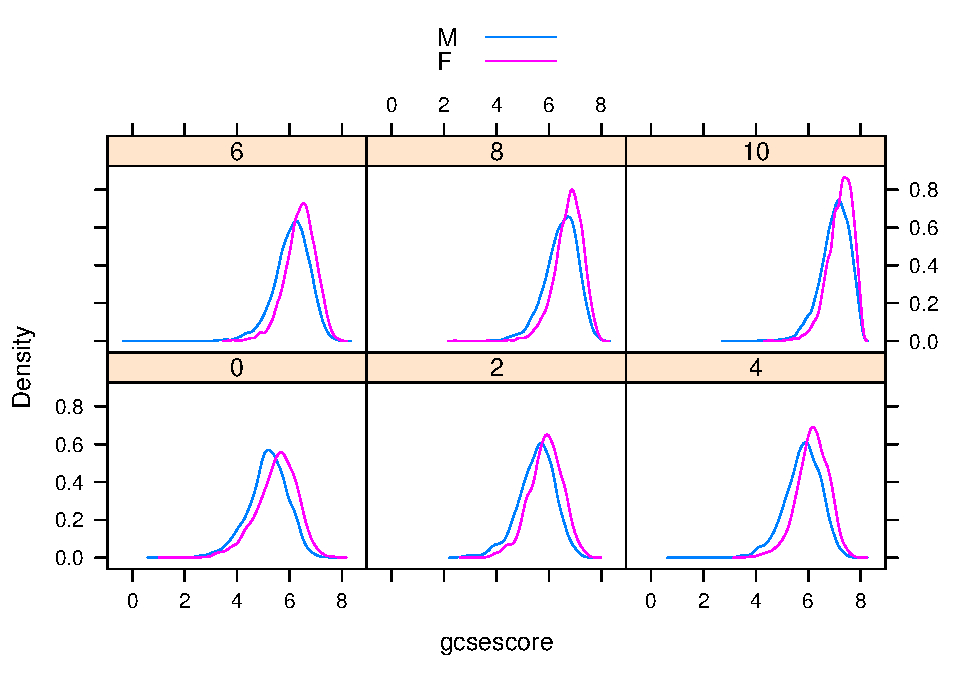
\includegraphics{Intro_Datenanalyse1_files/figure-latex/unnamed-chunk-173-1.pdf}

\href{http://www.isid.ac.in/~deepayan/R-tutorials/labs/04_lattice_lab.pdf}{Einführung
in das Paket lattice}

\subsection{Boxplot mit Lattice
zeichnen}\label{boxplot-mit-lattice-zeichnen}

\begin{Shaded}
\begin{Highlighting}[]
\KeywordTok{bwplot}\NormalTok{(}\KeywordTok{factor}\NormalTok{(score) ~}\StringTok{ }\NormalTok{gcsescore |}\StringTok{ }\NormalTok{gender, Chem97)}
\end{Highlighting}
\end{Shaded}

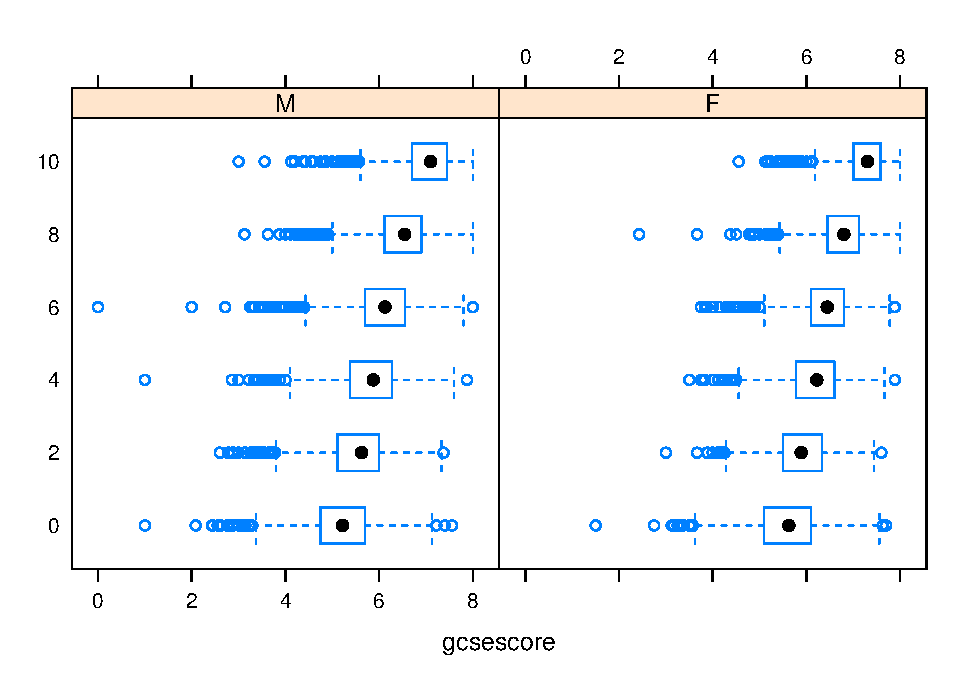
\includegraphics{Intro_Datenanalyse1_files/figure-latex/unnamed-chunk-174-1.pdf}

\subsection{Boxplot mit Lattice
zeichnen}\label{boxplot-mit-lattice-zeichnen-1}

\begin{Shaded}
\begin{Highlighting}[]
\KeywordTok{bwplot}\NormalTok{(gcsescore ~}\StringTok{ }\NormalTok{gender |}\StringTok{ }\KeywordTok{factor}\NormalTok{(score), Chem97,}
 \DataTypeTok{layout =} \KeywordTok{c}\NormalTok{(}\DecValTok{6}\NormalTok{, }\DecValTok{1}\NormalTok{))}
\end{Highlighting}
\end{Shaded}

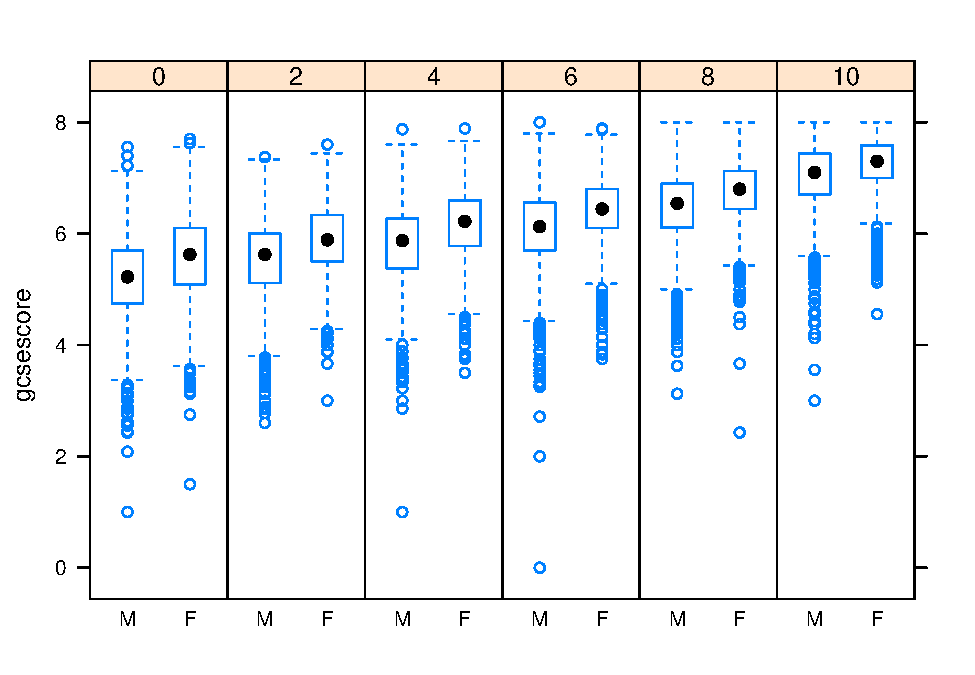
\includegraphics{Intro_Datenanalyse1_files/figure-latex/unnamed-chunk-175-1.pdf}

\subsection{Univariate Plots}\label{univariate-plots}

\begin{Shaded}
\begin{Highlighting}[]
\KeywordTok{barchart}\NormalTok{(yield ~}\StringTok{ }\NormalTok{variety |}\StringTok{ }\NormalTok{site, }\DataTypeTok{data =} \NormalTok{barley,}
         \DataTypeTok{groups =} \NormalTok{year, }\DataTypeTok{layout =} \KeywordTok{c}\NormalTok{(}\DecValTok{1}\NormalTok{,}\DecValTok{6}\NormalTok{), }\DataTypeTok{stack =} \OtherTok{TRUE}\NormalTok{,}
         \DataTypeTok{auto.key =} \KeywordTok{list}\NormalTok{(}\DataTypeTok{space =} \StringTok{"right"}\NormalTok{),}
         \DataTypeTok{ylab =} \StringTok{"Barley Yield (bushels/acre)"}\NormalTok{,}
         \DataTypeTok{scales =} \KeywordTok{list}\NormalTok{(}\DataTypeTok{x =} \KeywordTok{list}\NormalTok{(}\DataTypeTok{rot =} \DecValTok{45}\NormalTok{)))}
\end{Highlighting}
\end{Shaded}

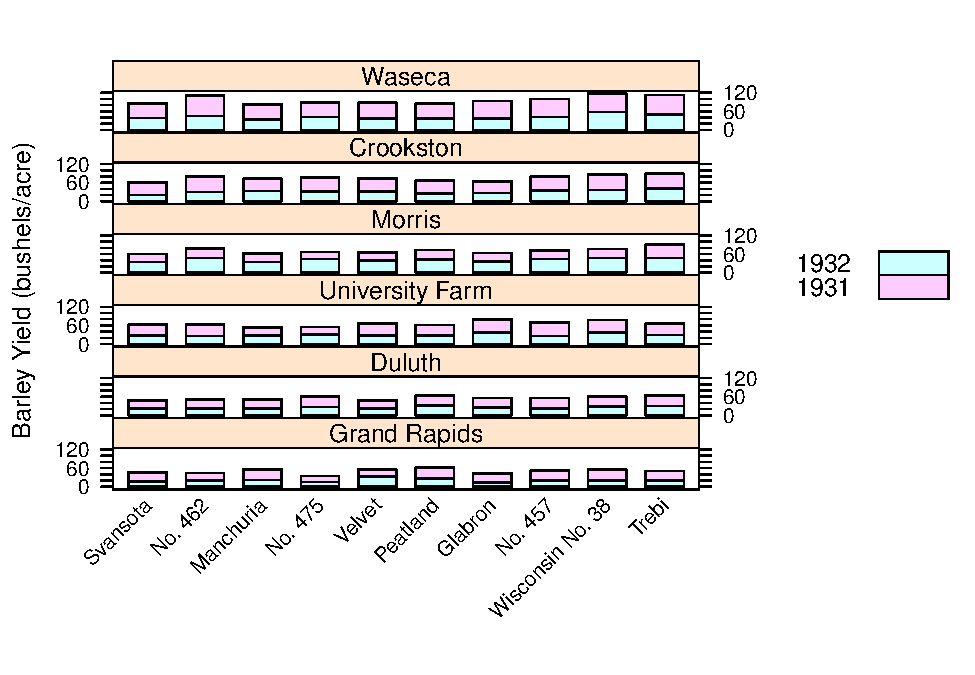
\includegraphics{Intro_Datenanalyse1_files/figure-latex/unnamed-chunk-176-1.pdf}

\subsection{Densityplot}\label{densityplot}

\begin{Shaded}
\begin{Highlighting}[]
\KeywordTok{densityplot}\NormalTok{( ~}\StringTok{ }\NormalTok{height |}\StringTok{ }\NormalTok{voice.part, }\DataTypeTok{data =} \NormalTok{singer, }\DataTypeTok{layout =} \KeywordTok{c}\NormalTok{(}\DecValTok{2}\NormalTok{, }\DecValTok{4}\NormalTok{),  }
            \DataTypeTok{xlab =} \StringTok{"Height (inches)"}\NormalTok{, }\DataTypeTok{bw =} \DecValTok{5}\NormalTok{)}
\end{Highlighting}
\end{Shaded}

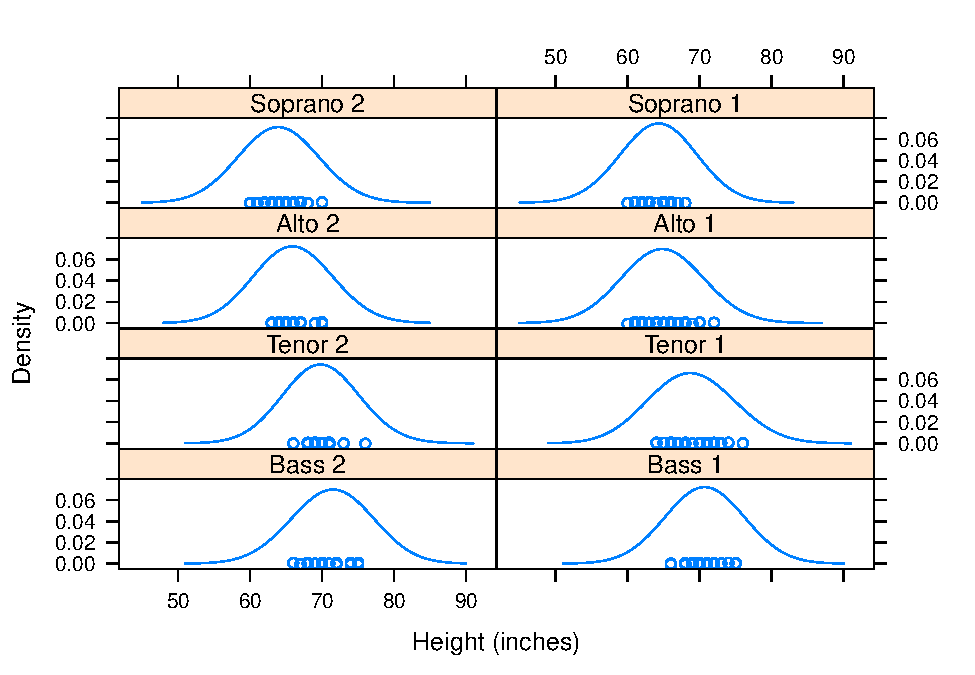
\includegraphics{Intro_Datenanalyse1_files/figure-latex/unnamed-chunk-177-1.pdf}

\subsection{Bivariate Plots}\label{bivariate-plots}

\begin{Shaded}
\begin{Highlighting}[]
\KeywordTok{qq}\NormalTok{(gender ~}\StringTok{ }\NormalTok{gcsescore |}\StringTok{ }\KeywordTok{factor}\NormalTok{(score), Chem97,}
   \DataTypeTok{f.value =} \KeywordTok{ppoints}\NormalTok{(}\DecValTok{100}\NormalTok{), }\DataTypeTok{type =} \KeywordTok{c}\NormalTok{(}\StringTok{"p"}\NormalTok{, }\StringTok{"g"}\NormalTok{), }\DataTypeTok{aspect =} \DecValTok{1}\NormalTok{)}
\end{Highlighting}
\end{Shaded}

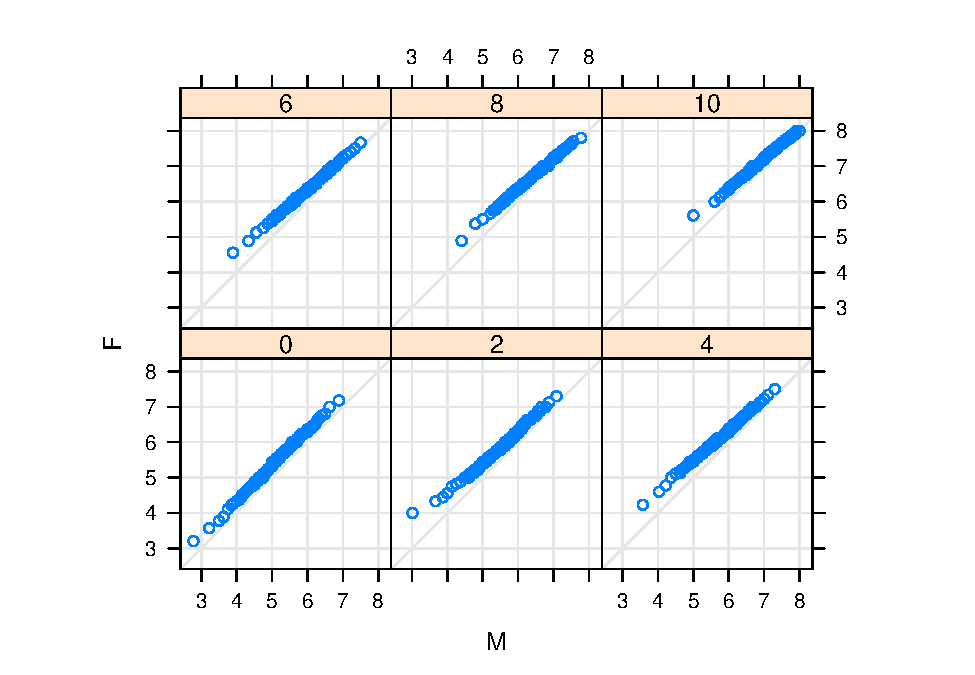
\includegraphics{Intro_Datenanalyse1_files/figure-latex/unnamed-chunk-178-1.pdf}

\subsection{xyplot}\label{xyplot}

\begin{Shaded}
\begin{Highlighting}[]
\KeywordTok{xyplot}\NormalTok{(Sepal.Length +}\StringTok{ }\NormalTok{Sepal.Width ~}\StringTok{ }\NormalTok{Petal.Length +}\StringTok{ }\NormalTok{Petal.Width |}\StringTok{ }\NormalTok{Species,}
       \DataTypeTok{data =} \NormalTok{iris, }\DataTypeTok{scales =} \StringTok{"free"}\NormalTok{, }\DataTypeTok{layout =} \KeywordTok{c}\NormalTok{(}\DecValTok{2}\NormalTok{, }\DecValTok{2}\NormalTok{),}
       \DataTypeTok{auto.key =} \KeywordTok{list}\NormalTok{(}\DataTypeTok{x =} \NormalTok{.}\DecValTok{6}\NormalTok{, }\DataTypeTok{y =} \NormalTok{.}\DecValTok{7}\NormalTok{, }\DataTypeTok{corner =} \KeywordTok{c}\NormalTok{(}\DecValTok{0}\NormalTok{, }\DecValTok{0}\NormalTok{)))}
\end{Highlighting}
\end{Shaded}

\includegraphics{Intro_Datenanalyse1_files/figure-latex/unnamed-chunk-179-1.pdf}

\subsection{Multivariate Plots}\label{multivariate-plots}

\begin{Shaded}
\begin{Highlighting}[]
\KeywordTok{splom}\NormalTok{(~iris[}\DecValTok{1}\NormalTok{:}\DecValTok{4}\NormalTok{], }\DataTypeTok{groups =} \NormalTok{Species, }\DataTypeTok{data =} \NormalTok{iris)}
\end{Highlighting}
\end{Shaded}

\includegraphics{Intro_Datenanalyse1_files/figure-latex/unnamed-chunk-180-1.pdf}

\begin{Shaded}
\begin{Highlighting}[]
\NormalTok{super.sym <-}\StringTok{ }\KeywordTok{trellis.par.get}\NormalTok{(}\StringTok{"superpose.symbol"}\NormalTok{)}
\KeywordTok{splom}\NormalTok{(~iris[}\DecValTok{1}\NormalTok{:}\DecValTok{4}\NormalTok{], }\DataTypeTok{groups =} \NormalTok{Species, }\DataTypeTok{data =} \NormalTok{iris,}
      \DataTypeTok{panel =} \NormalTok{panel.superpose,}
      \DataTypeTok{key =} \KeywordTok{list}\NormalTok{(}\DataTypeTok{title =} \StringTok{"Three Varieties of Iris"}\NormalTok{,}
                 \DataTypeTok{columns =} \DecValTok{3}\NormalTok{, }
                 \DataTypeTok{points =} \KeywordTok{list}\NormalTok{(}\DataTypeTok{pch =} \NormalTok{super.sym$pch[}\DecValTok{1}\NormalTok{:}\DecValTok{3}\NormalTok{],}
                 \DataTypeTok{col =} \NormalTok{super.sym$col[}\DecValTok{1}\NormalTok{:}\DecValTok{3}\NormalTok{]),}
                 \DataTypeTok{text =} \KeywordTok{list}\NormalTok{(}\KeywordTok{c}\NormalTok{(}\StringTok{"Setosa"}\NormalTok{, }\StringTok{"Versicolor"}\NormalTok{, }\StringTok{"Virginica"}\NormalTok{))))}
\end{Highlighting}
\end{Shaded}

\includegraphics{Intro_Datenanalyse1_files/figure-latex/unnamed-chunk-181-1.pdf}

\subsection{parallelplot}\label{parallelplot}

\begin{Shaded}
\begin{Highlighting}[]
\KeywordTok{parallelplot}\NormalTok{(~iris[}\DecValTok{1}\NormalTok{:}\DecValTok{4}\NormalTok{] |}\StringTok{ }\NormalTok{Species, iris)}
\end{Highlighting}
\end{Shaded}

\includegraphics{Intro_Datenanalyse1_files/figure-latex/unnamed-chunk-182-1.pdf}

\subsection{Lattice Befehle}\label{lattice-befehle}

\begin{itemize}
\tightlist
\item
  \href{http://www.isid.ac.in/~deepayan/R-tutorials/labs/04_lattice_lab.pdf}{Übersicht
  aller Lattice Befehle}
\end{itemize}

\subsection{Aufgabe - OECD Datensatz}\label{aufgabe---oecd-datensatz}

\begin{itemize}
\tightlist
\item
  Laden Sie den oecd-Datensatz herunter und lesen Sie ihn mit folgender
  Funktion ein:
\end{itemize}

\begin{Shaded}
\begin{Highlighting}[]
\NormalTok{data <-}\StringTok{ }\KeywordTok{read.csv}\NormalTok{(}\StringTok{"oecd.csv"}\NormalTok{,}\DataTypeTok{header =} \OtherTok{TRUE}\NormalTok{)}
\end{Highlighting}
\end{Shaded}

\begin{itemize}
\item
  Überprüfen Sie die Dimension der OECD-Daten.
\item
  Berechnen Sie die Mittelwerte und Varianzen der einzelnen Variablen
  mit einem geeigneten apply Befehl.
\item
  In welchem Land waren die meisten Jugendlichen mindestens zweimal
  betrunken? Wie hoch ist der maximale Prozentsatz?
\item
  In welchem Land ist die Sterblichkeit am geringsten? Wie hoch ist sie
  in diesem Land?
\item
  Erstellen Sie einen neuen Datensatz, der aufsteigend nach dem
  Einkommen geordnet ist. Speichern Sie diesen in einer neuen .csv Datei
\end{itemize}

\href{https://github.com/Japhilko/IntroR/blob/master/2017/README.md}{Zurück
zur Gliederung.}

\section{Die lineare Regression}\label{die-lineare-regression}

\subsection{Die lineare Regression}\label{die-lineare-regression-1}

Maindonald -
\href{https://cran.r-project.org/doc/contrib/usingR.pdf}{DataAnalysis}

\begin{itemize}
\tightlist
\item
  Einführung in R
\item
  Datenanalyse
\item
  Statistische Modelle
\item
  Inferenzkonzepte
\item
  Regression mit einem Prädiktor
\item
  Multiple lineare Regression
\item
  Ausweitung des linearen Modells
\item
  \ldots{}
\end{itemize}

\subsection{Lineare Regression in R -
Beispieldatensatz}\label{lineare-regression-in-r---beispieldatensatz}

John H. Maindonald and W. John Braun

DAAG -
\href{http://cran.ms.unimelb.edu.au/web/packages/DAAG/DAAG.pdf}{Data
Analysis and Graphics Data and Functions}

\begin{Shaded}
\begin{Highlighting}[]
\KeywordTok{install.packages}\NormalTok{(}\StringTok{"DAAG"}\NormalTok{)}
\end{Highlighting}
\end{Shaded}

\begin{Shaded}
\begin{Highlighting}[]
\KeywordTok{library}\NormalTok{(}\StringTok{"DAAG"}\NormalTok{)}
\KeywordTok{data}\NormalTok{(roller)}
\end{Highlighting}
\end{Shaded}

help on roller data:

\begin{Shaded}
\begin{Highlighting}[]
\NormalTok{?roller}
\end{Highlighting}
\end{Shaded}

\subsection{Das lineare Regressionsmodell in
R}\label{das-lineare-regressionsmodell-in-r}

Schätzen eines Regressionsmodells:

\begin{Shaded}
\begin{Highlighting}[]
\NormalTok{roller.lm <-}\StringTok{ }\KeywordTok{lm}\NormalTok{(depression ~}\StringTok{ }\NormalTok{weight, }\DataTypeTok{data =} \NormalTok{roller)}
\end{Highlighting}
\end{Shaded}

So bekommt man die Schätzwerte:

\begin{Shaded}
\begin{Highlighting}[]
\KeywordTok{summary}\NormalTok{(roller.lm)}
\end{Highlighting}
\end{Shaded}

\begin{verbatim}
## 
## Call:
## lm(formula = depression ~ weight, data = roller)
## 
## Residuals:
##    Min     1Q Median     3Q    Max 
## -8.180 -5.580 -1.346  5.920  8.020 
## 
## Coefficients:
##             Estimate Std. Error t value Pr(>|t|)   
## (Intercept)  -2.0871     4.7543  -0.439  0.67227   
## weight        2.6667     0.7002   3.808  0.00518 **
## ---
## Signif. codes:  0 '***' 0.001 '**' 0.01 '*' 0.05 '.' 0.1 ' ' 1
## 
## Residual standard error: 6.735 on 8 degrees of freedom
## Multiple R-squared:  0.6445, Adjusted R-squared:  0.6001 
## F-statistic:  14.5 on 1 and 8 DF,  p-value: 0.005175
\end{verbatim}

Falls das Modell ohne Intercept geschätzt werden soll:

\begin{Shaded}
\begin{Highlighting}[]
\KeywordTok{lm}\NormalTok{(depression ~}\StringTok{ }\NormalTok{-}\DecValTok{1} \NormalTok{+}\StringTok{ }\NormalTok{weight, }\DataTypeTok{data =} \NormalTok{roller)}
\end{Highlighting}
\end{Shaded}

\begin{verbatim}
## 
## Call:
## lm(formula = depression ~ -1 + weight, data = roller)
## 
## Coefficients:
## weight  
##  2.392
\end{verbatim}

\subsection{Summary des Modells}\label{summary-des-modells}

\begin{Shaded}
\begin{Highlighting}[]
\KeywordTok{summary}\NormalTok{(roller.lm)}
\end{Highlighting}
\end{Shaded}

\begin{verbatim}
## 
## Call:
## lm(formula = depression ~ weight, data = roller)
## 
## Residuals:
##    Min     1Q Median     3Q    Max 
## -8.180 -5.580 -1.346  5.920  8.020 
## 
## Coefficients:
##             Estimate Std. Error t value Pr(>|t|)   
## (Intercept)  -2.0871     4.7543  -0.439  0.67227   
## weight        2.6667     0.7002   3.808  0.00518 **
## ---
## Signif. codes:  0 '***' 0.001 '**' 0.01 '*' 0.05 '.' 0.1 ' ' 1
## 
## Residual standard error: 6.735 on 8 degrees of freedom
## Multiple R-squared:  0.6445, Adjusted R-squared:  0.6001 
## F-statistic:  14.5 on 1 and 8 DF,  p-value: 0.005175
\end{verbatim}

\subsection{R arbeitet mit Objekten}\label{r-arbeitet-mit-objekten}

\begin{itemize}
\tightlist
\item
  \texttt{roller.lm} ist nun ein spezielles Regressions-Objekt
\item
  Auf dieses Objekt können nun verschiedene Funktionen angewendet werden
\end{itemize}

\begin{Shaded}
\begin{Highlighting}[]
\KeywordTok{predict}\NormalTok{(roller.lm) }\CommentTok{# Vorhersage}
\end{Highlighting}
\end{Shaded}

\begin{verbatim}
##         1         2         3         4         5         6         7 
##  2.979669  6.179765  6.713114 10.713233 12.046606 14.180002 14.980026 
##         8         9        10 
## 18.180121 24.046962 30.980502
\end{verbatim}

\begin{Shaded}
\begin{Highlighting}[]
\KeywordTok{resid}\NormalTok{(roller.lm) }\CommentTok{# Residuen}
\end{Highlighting}
\end{Shaded}

\begin{verbatim}
##          1          2          3          4          5          6 
## -0.9796695 -5.1797646 -1.7131138 -5.7132327  7.9533944  5.8199976 
##          7          8          9         10 
##  8.0199738 -8.1801213  5.9530377 -5.9805017
\end{verbatim}

\subsection{Residuenplot}\label{residuenplot}

\begin{itemize}
\tightlist
\item
  Sind Annahmen des linearen Regressionsmodells verletzt?
\item
  Dies ist der Fall, wenn ein Muster abweichend von einer Linie zu
  erkennen ist.
\item
  Hier ist der Datensatz sehr klein
\end{itemize}

\begin{Shaded}
\begin{Highlighting}[]
\KeywordTok{plot}\NormalTok{(roller.lm,}\DecValTok{1}\NormalTok{)}
\end{Highlighting}
\end{Shaded}

\includegraphics{Intro_Datenanalyse1_files/figure-latex/unnamed-chunk-193-1.pdf}

\subsection{Residuenplot}\label{residuenplot-1}

\begin{Shaded}
\begin{Highlighting}[]
\KeywordTok{plot}\NormalTok{(roller.lm,}\DecValTok{2}\NormalTok{)}
\end{Highlighting}
\end{Shaded}

\includegraphics{Intro_Datenanalyse1_files/figure-latex/unnamed-chunk-194-1.pdf}

\begin{itemize}
\tightlist
\item
  Wenn die Residuen normalverteilt sind sollten sie auf einer Linie
  liegen.
\end{itemize}

\subsection{Linkliste - lineare
Regression}\label{linkliste---lineare-regression}

\begin{itemize}
\item
  Regression -
  \href{http://www.r-bloggers.com/r-tutorial-series-simple-linear-regression/}{r-bloggers}
\item
  Das Komplette Buch von
  \href{http://cran.r-project.org/doc/contrib/Faraway-PRA.pdf}{Faraway}-
  sehr intuitiv geschrieben.
\item
  Gute Einführung auf
  \href{http://www.statmethods.net/stats/regression.html}{Quick-R}
\item
  \href{https://www.r-bloggers.com/multiple-regression-part-1/}{Multiple
  Regression}
\end{itemize}

\subsection{Aufgabe - lineare
Regression}\label{aufgabe---lineare-regression}

Beschrieben wird Wegstrecke, dreier Spielzeugautos die in
unterschiedlichen Winkeln Rampe herunterfuhren.

\begin{itemize}
\tightlist
\item
  angle: Winkel der Rampe
\item
  distance: Zurückgelegte Strecke des Spielzeugautos
\item
  car: Autotyp (1, 2 oder 3)
\end{itemize}

\begin{enumerate}
\def\labelenumi{(\alph{enumi})}
\item
  Lesen Sie den Datensatz \texttt{toycars} in einen dataframe data ein
  und wandeln Sie die Variable car des Datensatzes in einen Faktor
  (\texttt{as.factor}) um.
\item
  Erstellen Sie drei Boxplots, die die zurückgelegte Strecke getrennt
  nach dem Faktor car darstellen.
\item
  Schätzen Sie für jedes der 3 Autos separat die Parameter des folgenden
  linearen Mo dells mit Hilfe der Funktion lm()
\end{enumerate}

\[ distance_i= \beta_0 + \beta_1 \cdot angle_i + \epsilon_i\]

\begin{enumerate}
\def\labelenumi{(\alph{enumi})}
\setcounter{enumi}{3}
\tightlist
\item
  Überprüfen Sie deskriptiv die Anpassung der drei Modelle, indem Sie
  die Regressionger- ade in einen Plot von distance gegen angle
  einfügen. Deutet das \[ R^2 \] jeweils auf eine gute Modellanpassung
  hin?
\end{enumerate}

\href{https://github.com/Japhilko/IntroR/blob/master/2017/README.md}{Zurück
zur Gliederung.}

\section{Die logistische Regression}\label{die-logistische-regression}

\subsection{\texorpdfstring{Agresti -
\href{https://mathdept.iut.ac.ir/sites/mathdept.iut.ac.ir/files/AGRESTI.PDF}{Categorical
Data Analysis
(2002)}}{Agresti - Categorical Data Analysis (2002)}}\label{agresti---categorical-data-analysis-2002}

\begin{figure}[htbp]
\centering
\includegraphics{figure/CDAagresti.PNG}
\caption{}
\end{figure}

\begin{itemize}
\tightlist
\item
  Sehr intiutiv geschriebenes Buch
\item
  Sehr ausführliches begleitendes Skript von
  \href{http://statweb.stanford.edu/~owen/courses/306a/Splusdiscrete2.pdf}{Thompson}
\item
  Das Skript eignet sich um die kategoriale Datenanalyse
  nachzuvollziehen
\end{itemize}

\subsection{Faraway Bücher zu Regression in
R}\label{faraway-bucher-zu-regression-in-r}

\begin{figure}[htbp]
\centering
\includegraphics{figure/Faraway.PNG}
\caption{}
\end{figure}

\begin{itemize}
\item
  Logistische Regressionen gut erklärt
\item
  Beispiele mit R-code

  \begin{itemize}
  \item
    Faraway - Extending the linear model with r
  \item
    Faraway -
    \href{https://cran.r-project.org/doc/contrib/Faraway-PRA.pdf}{Practical
    Regression and Anova using R}
  \end{itemize}
\end{itemize}

\subsection{\texorpdfstring{Binäre AVs mit
\texttt{glm}}{Binäre AVs mit glm}}\label{binare-avs-mit-glm}

\begin{itemize}
\tightlist
\item
  Die \href{http://data.princeton.edu/R/glms.html}{logistische
  Regression} gehört zur Klasse der generalisierten linearen Modelle
  (GLM)
\item
  Die Funktion zur Schätzung eines Modells dieser Klasse in heißt
  \texttt{glm()}
\item
  \texttt{glm()} muss 1. ein Formel-Objekt mitgegeben werden und 2. die
  Klasse (binomial, gaussian, Gamma) samt link-Funktion (logit, probit,
  cauchit, log, cloglog)
\end{itemize}

\subsection{Beispieldaten für die logistische
Regression}\label{beispieldaten-fur-die-logistische-regression}

\begin{Shaded}
\begin{Highlighting}[]
\KeywordTok{install.packages}\NormalTok{(}\StringTok{"HSAUR"}\NormalTok{)}
\end{Highlighting}
\end{Shaded}

\begin{Shaded}
\begin{Highlighting}[]
\KeywordTok{library}\NormalTok{(}\StringTok{"HSAUR"}\NormalTok{)}
\KeywordTok{data}\NormalTok{(}\StringTok{"plasma"}\NormalTok{, }\DataTypeTok{package =} \StringTok{"HSAUR"}\NormalTok{)}
\end{Highlighting}
\end{Shaded}

\subsection{Logistische Regression mit
R}\label{logistische-regression-mit-r}

\begin{itemize}
\tightlist
\item
  \href{http://homepage.univie.ac.at/herbert.nagel/KategorialeDaten.pdf}{Kategoriale
  Daten:}
\end{itemize}

\begin{Shaded}
\begin{Highlighting}[]
\KeywordTok{cdplot}\NormalTok{(ESR ~}\StringTok{ }\NormalTok{fibrinogen, }\DataTypeTok{data =} \NormalTok{plasma)}
\end{Highlighting}
\end{Shaded}

\includegraphics{Intro_Datenanalyse1_files/figure-latex/unnamed-chunk-198-1.pdf}

\subsection{\texorpdfstring{\href{http://ww2.coastal.edu/kingw/statistics/R-tutorials/logistic.html}{Logistische
Regression} mit
R}{Logistische Regression mit R}}\label{logistische-regression-mit-r-1}

\begin{Shaded}
\begin{Highlighting}[]
\NormalTok{plasma_glm_1 <-}\StringTok{ }\KeywordTok{glm}\NormalTok{(ESR ~}\StringTok{ }\NormalTok{fibrinogen, }\DataTypeTok{data =} \NormalTok{plasma, }
                    \DataTypeTok{family =} \KeywordTok{binomial}\NormalTok{())}
\end{Highlighting}
\end{Shaded}

\subsection{Weitere Beispieldaten}\label{weitere-beispieldaten}

\begin{Shaded}
\begin{Highlighting}[]
\KeywordTok{install.packages}\NormalTok{(}\StringTok{"faraway"}\NormalTok{)}
\end{Highlighting}
\end{Shaded}

\begin{Shaded}
\begin{Highlighting}[]
\KeywordTok{library}\NormalTok{(}\StringTok{"faraway"}\NormalTok{)}
\end{Highlighting}
\end{Shaded}

\begin{Shaded}
\begin{Highlighting}[]
\KeywordTok{data}\NormalTok{(orings)}
\end{Highlighting}
\end{Shaded}

\begin{longtable}[]{@{}rr@{}}
\toprule
temp & damage\tabularnewline
\midrule
\endhead
53 & 5\tabularnewline
57 & 1\tabularnewline
58 & 1\tabularnewline
\bottomrule
\end{longtable}

\subsection{Generalisierte Regression mit R - weitere
Funktionen}\label{generalisierte-regression-mit-r---weitere-funktionen}

\begin{itemize}
\tightlist
\item
  Logistisches Modell mit Probit-Link:
\end{itemize}

\begin{Shaded}
\begin{Highlighting}[]
\NormalTok{probitmod <-}\StringTok{ }\KeywordTok{glm}\NormalTok{(}\KeywordTok{cbind}\NormalTok{(damage,}\DecValTok{6}\NormalTok{-damage) ~}\StringTok{ }\NormalTok{temp, }
    \DataTypeTok{family=}\KeywordTok{binomial}\NormalTok{(}\DataTypeTok{link=}\NormalTok{probit), orings)}
\end{Highlighting}
\end{Shaded}

\begin{itemize}
\tightlist
\item
  Regression mit Zähldaten:
\end{itemize}

\begin{Shaded}
\begin{Highlighting}[]
\NormalTok{modp <-}\StringTok{ }\KeywordTok{glm}\NormalTok{(Species ~}\StringTok{ }\NormalTok{.,}\DataTypeTok{family=}\NormalTok{poisson,gala)}
\end{Highlighting}
\end{Shaded}

\begin{itemize}
\tightlist
\item
  Proportional odds logistic regression im Paket \texttt{MASS}:
\end{itemize}

\begin{Shaded}
\begin{Highlighting}[]
\KeywordTok{library}\NormalTok{(}\StringTok{"MASS"}\NormalTok{)}
\NormalTok{house.plr<-}\KeywordTok{polr}\NormalTok{(Sat~Infl,}\DataTypeTok{weights=}\NormalTok{Freq,}\DataTypeTok{data=}\NormalTok{housing)}
\end{Highlighting}
\end{Shaded}

\subsection{Linkliste - logistische
Regression}\label{linkliste---logistische-regression}

\begin{itemize}
\tightlist
\item
  Einführung in
  \href{http://ww2.coastal.edu/kingw/statistics/R-tutorials/logistic.html}{logistische
  Regression}
\end{itemize}

\begin{figure}[htbp]
\centering
\includegraphics{figure/Rtutorials.PNG}
\caption{}
\end{figure}

\begin{itemize}
\tightlist
\item
  \href{http://www.maths.bath.ac.uk/~jjf23/ELM/scripts/binary.R}{Code
  zum Buch von Faraway}
\end{itemize}

\begin{figure}[htbp]
\centering
\includegraphics{figure/orings.PNG}
\caption{}
\end{figure}

\subsection{Aufgabe - Datenanalyse}\label{aufgabe---datenanalyse}

\begin{itemize}
\tightlist
\item
  Laden Sie einen Datensatz Ihrer Wahl - entweder einen eigenen oder
  einen der vorgestellten Datensätze
\item
  Berechnen Sie einfache Statistiken auf den wichtigsten Variablen
  (Mittelwert, Median, Standardabweichung)
\item
  Erzeugen Sie eine zweidimensionale Häufigkeitstabelle
\item
  Führen Sie eine Regression mit sinnvoll gewählten abhängiger und
  unabhängiger Variablen auf den Daten durch
\item
  Erzeugen Sie einen Lattice-plot
\end{itemize}

\href{https://github.com/Japhilko/IntroR/blob/master/2017/README.md}{Zurück
zur Gliederung.}

\section{Faktoren in R}\label{faktoren-in-r}

\subsection{Was sind Faktoren in R}\label{was-sind-faktoren-in-r}

\begin{itemize}
\tightlist
\item
  Faktoren können eine begrenzte Zahl von Ausprägungen annehmen
\item
  Sie werden oft auch als kategoriale Variablen bezeichnet
\item
  Sie sind vor allem bei der Modellierung wichtig
\item
  Faktoren werden anders behandelt als stetige Variablen
\item
  Wenn man diese Variablen richtig definiert werden sie auch von R
  richtig behandelt
\end{itemize}

\url{http://www.stat.berkeley.edu/~s133/factors.html}

\subsection{Beispiel Definition von
Faktoren}\label{beispiel-definition-von-faktoren}

\begin{Shaded}
\begin{Highlighting}[]
\NormalTok{data <-}\StringTok{ }\KeywordTok{c}\NormalTok{(}\DecValTok{1}\NormalTok{,}\DecValTok{2}\NormalTok{,}\DecValTok{2}\NormalTok{,}\DecValTok{3}\NormalTok{,}\DecValTok{1}\NormalTok{,}\DecValTok{2}\NormalTok{,}\DecValTok{3}\NormalTok{,}\DecValTok{3}\NormalTok{,}\DecValTok{1}\NormalTok{,}\DecValTok{2}\NormalTok{,}\DecValTok{3}\NormalTok{,}\DecValTok{3}\NormalTok{,}\DecValTok{1}\NormalTok{)}
\NormalTok{fdata <-}\StringTok{ }\KeywordTok{factor}\NormalTok{(data)}
\NormalTok{fdata}
\end{Highlighting}
\end{Shaded}

\begin{verbatim}
##  [1] 1 2 2 3 1 2 3 3 1 2 3 3 1
## Levels: 1 2 3
\end{verbatim}

\begin{itemize}
\tightlist
\item
  \texttt{labels} direkt definieren
\end{itemize}

\begin{Shaded}
\begin{Highlighting}[]
\NormalTok{rdata <-}\StringTok{ }\KeywordTok{factor}\NormalTok{(data,}\DataTypeTok{labels=}\KeywordTok{c}\NormalTok{(}\StringTok{"I"}\NormalTok{,}\StringTok{"II"}\NormalTok{,}\StringTok{"III"}\NormalTok{))}
\NormalTok{rdata}
\end{Highlighting}
\end{Shaded}

\begin{verbatim}
##  [1] I   II  II  III I   II  III III I   II  III III I  
## Levels: I II III
\end{verbatim}

\subsection{Weitere Möglichkeit der
Definition}\label{weitere-moglichkeit-der-definition}

\begin{Shaded}
\begin{Highlighting}[]
\KeywordTok{levels}\NormalTok{(fdata) <-}\StringTok{ }\KeywordTok{c}\NormalTok{(}\StringTok{'I'}\NormalTok{,}\StringTok{'II'}\NormalTok{,}\StringTok{'III'}\NormalTok{)}
\NormalTok{fdata}
\end{Highlighting}
\end{Shaded}

\begin{verbatim}
##  [1] I   II  II  III I   II  III III I   II  III III I  
## Levels: I II III
\end{verbatim}

\subsection{Beispiel Monate}\label{beispiel-monate}

\begin{Shaded}
\begin{Highlighting}[]
\NormalTok{mons <-}\StringTok{ }\KeywordTok{c}\NormalTok{(}\StringTok{"March"}\NormalTok{,}\StringTok{"April"}\NormalTok{,}\StringTok{"January"}\NormalTok{,}
          \StringTok{"November"}\NormalTok{,}\StringTok{"January"}\NormalTok{,}\StringTok{"September"}\NormalTok{,}
          \StringTok{"October"}\NormalTok{,}\StringTok{"September"}\NormalTok{,}\StringTok{"November"}\NormalTok{,}
          \StringTok{"August"}\NormalTok{,}\StringTok{"January"}\NormalTok{,}\StringTok{"November"}\NormalTok{,}
          \StringTok{"November"}\NormalTok{,}\StringTok{"February"}\NormalTok{,}\StringTok{"May"}\NormalTok{,}
          \StringTok{"August"}\NormalTok{,}\StringTok{"July"}\NormalTok{,}\StringTok{"December"}\NormalTok{,}
          \StringTok{"August"}\NormalTok{,}\StringTok{"August"}\NormalTok{,}\StringTok{"September"}\NormalTok{,}
          \StringTok{"November"}\NormalTok{,}\StringTok{"February"}\NormalTok{,}\StringTok{"April"}\NormalTok{)}
\NormalTok{mons <-}\StringTok{ }\KeywordTok{factor}\NormalTok{(mons)}
\KeywordTok{table}\NormalTok{(mons)}
\end{Highlighting}
\end{Shaded}

\begin{verbatim}
## mons
##     April    August  December  February   January      July     March 
##         2         4         1         2         3         1         1 
##       May  November   October September 
##         1         5         1         3
\end{verbatim}

\subsection{Beispiel: ordered factor}\label{beispiel-ordered-factor}

\begin{Shaded}
\begin{Highlighting}[]
\NormalTok{mons <-}\StringTok{ }\KeywordTok{factor}\NormalTok{(mons,}\DataTypeTok{levels=}\KeywordTok{c}\NormalTok{(}\StringTok{"January"}\NormalTok{,}\StringTok{"February"}\NormalTok{,}
                             \StringTok{"March"}\NormalTok{,}\StringTok{"April"}\NormalTok{,}\StringTok{"May"}\NormalTok{,}\StringTok{"June"}\NormalTok{,}
                             \StringTok{"July"}\NormalTok{,}\StringTok{"August"}\NormalTok{,}\StringTok{"September"}\NormalTok{,  }
                             \StringTok{"October"}\NormalTok{,}\StringTok{"November"}\NormalTok{,}
                             \StringTok{"December"}\NormalTok{),}
               \DataTypeTok{ordered=}\OtherTok{TRUE}\NormalTok{)}

\NormalTok{mons[}\DecValTok{1}\NormalTok{] <}\StringTok{ }\NormalTok{mons[}\DecValTok{2}\NormalTok{]}
\end{Highlighting}
\end{Shaded}

\begin{verbatim}
## [1] TRUE
\end{verbatim}

\subsection{Rücktransformation}\label{rucktransformation}

\begin{Shaded}
\begin{Highlighting}[]
\NormalTok{fert <-}\StringTok{ }\KeywordTok{c}\NormalTok{(}\DecValTok{10}\NormalTok{,}\DecValTok{20}\NormalTok{,}\DecValTok{20}\NormalTok{,}\DecValTok{50}\NormalTok{,}\DecValTok{10}\NormalTok{,}\DecValTok{20}\NormalTok{,}\DecValTok{10}\NormalTok{,}\DecValTok{50}\NormalTok{,}\DecValTok{20}\NormalTok{)}
\NormalTok{fert <-}\StringTok{ }\KeywordTok{factor}\NormalTok{(fert,}\DataTypeTok{levels=}\KeywordTok{c}\NormalTok{(}\DecValTok{10}\NormalTok{,}\DecValTok{20}\NormalTok{,}\DecValTok{50}\NormalTok{),}\DataTypeTok{ordered=}\OtherTok{TRUE}\NormalTok{)}
\NormalTok{fert}
\end{Highlighting}
\end{Shaded}

\begin{verbatim}
## [1] 10 20 20 50 10 20 10 50 20
## Levels: 10 < 20 < 50
\end{verbatim}

\begin{Shaded}
\begin{Highlighting}[]
\KeywordTok{mean}\NormalTok{(fert)}
\end{Highlighting}
\end{Shaded}

\begin{verbatim}
## [1] NA
\end{verbatim}

\begin{Shaded}
\begin{Highlighting}[]
\KeywordTok{mean}\NormalTok{(}\KeywordTok{as.numeric}\NormalTok{(}\KeywordTok{levels}\NormalTok{(fert)[fert]))}
\end{Highlighting}
\end{Shaded}

\begin{verbatim}
## [1] 23.33333
\end{verbatim}

\subsection{Tabellen mit Faktoren}\label{tabellen-mit-faktoren}

\begin{Shaded}
\begin{Highlighting}[]
\NormalTok{lets <-}\StringTok{ }\KeywordTok{sample}\NormalTok{(letters,}\DataTypeTok{size=}\DecValTok{100}\NormalTok{,}\DataTypeTok{replace=}\OtherTok{TRUE}\NormalTok{)}
\NormalTok{lets <-}\StringTok{ }\KeywordTok{factor}\NormalTok{(lets)}
\KeywordTok{table}\NormalTok{(lets[}\DecValTok{1}\NormalTok{:}\DecValTok{5}\NormalTok{])}
\end{Highlighting}
\end{Shaded}

\begin{verbatim}
## 
## a b c d e f g h i k l m n o p q r s t u v w x y z 
## 0 0 0 0 0 1 0 0 2 1 0 0 0 0 0 0 0 0 0 0 0 0 0 1 0
\end{verbatim}

\section{Grafiken mit ggplot}\label{grafiken-mit-ggplot}

\subsection{\texorpdfstring{Das Paket
\texttt{ggplot2}}{Das Paket ggplot2}}\label{das-paket-ggplot2}

\begin{itemize}
\tightlist
\item
  Entwickelt von Hadley Wickham
\item
  Viele Informationen unter:
\item
  \url{http://ggplot2.org/}
\item
  Den Graphiken liegt eine eigene Grammitik zu Grunde
\end{itemize}

\begin{figure}[htbp]
\centering
\includegraphics{figure/GalleryGGplot2.PNG}
\caption{}
\end{figure}

\subsection{\texorpdfstring{\href{www.r-bloggers.com/basic-introduction-to-ggplot2/}{Basiseinführung
\texttt{ggplot2}}}{Basiseinführung ggplot2}}\label{basiseinfuhrung-ggplot2}

\textless{}www.r-bloggers.com/basic-introduction-to-ggplot2/\textgreater{}

\begin{Shaded}
\begin{Highlighting}[]
\KeywordTok{install.packages}\NormalTok{(}\StringTok{"ggplot2"}\NormalTok{)}
\end{Highlighting}
\end{Shaded}

\begin{Shaded}
\begin{Highlighting}[]
\KeywordTok{library}\NormalTok{(ggplot2)}
\end{Highlighting}
\end{Shaded}

\subsection{\texorpdfstring{Der \texttt{diamonds}
Datensatz}{Der diamonds Datensatz}}\label{der-diamonds-datensatz}

\begin{Shaded}
\begin{Highlighting}[]
\KeywordTok{head}\NormalTok{(diamonds)}
\end{Highlighting}
\end{Shaded}

\begin{longtable}[]{@{}rlllrrrrrr@{}}
\toprule
carat & cut & color & clarity & depth & table & price & x & y &
z\tabularnewline
\midrule
\endhead
0.23 & Ideal & E & SI2 & 61.5 & 55 & 326 & 3.95 & 3.98 &
2.43\tabularnewline
0.21 & Premium & E & SI1 & 59.8 & 61 & 326 & 3.89 & 3.84 &
2.31\tabularnewline
0.23 & Good & E & VS1 & 56.9 & 65 & 327 & 4.05 & 4.07 &
2.31\tabularnewline
0.29 & Premium & I & VS2 & 62.4 & 58 & 334 & 4.20 & 4.23 &
2.63\tabularnewline
0.31 & Good & J & SI2 & 63.3 & 58 & 335 & 4.34 & 4.35 &
2.75\tabularnewline
0.24 & Very Good & J & VVS2 & 62.8 & 57 & 336 & 3.94 & 3.96 &
2.48\tabularnewline
\bottomrule
\end{longtable}

\subsection{\texorpdfstring{Wie nutzt man
\texttt{qplot}}{Wie nutzt man qplot}}\label{wie-nutzt-man-qplot}

\begin{itemize}
\tightlist
\item
  Die Funktion \texttt{qplot} wird für schnelle Graphiken verwendet
  (quick plots)
\item
  bei der Funktion \texttt{ggplot} kann man alles bis ins Detail
  kontrollieren
\end{itemize}

\begin{Shaded}
\begin{Highlighting}[]
\CommentTok{# histogram}
\KeywordTok{qplot}\NormalTok{(depth, }\DataTypeTok{data=}\NormalTok{diamonds)}
\end{Highlighting}
\end{Shaded}

\includegraphics{Intro_Datenanalyse1_files/figure-latex/unnamed-chunk-220-1.pdf}

\subsection{Ein Balkendiagramm}\label{ein-balkendiagramm}

\begin{Shaded}
\begin{Highlighting}[]
\KeywordTok{qplot}\NormalTok{(cut, depth, }\DataTypeTok{data=}\NormalTok{diamonds)}
\end{Highlighting}
\end{Shaded}

\includegraphics{Intro_Datenanalyse1_files/figure-latex/unnamed-chunk-221-1.pdf}

\subsection{Ein weiteres
Balkendiagramm}\label{ein-weiteres-balkendiagramm}

\begin{Shaded}
\begin{Highlighting}[]
\KeywordTok{qplot}\NormalTok{(}\KeywordTok{factor}\NormalTok{(cyl), }\DataTypeTok{data=}\NormalTok{mtcars,}\DataTypeTok{geom=}\StringTok{"bar"}\NormalTok{)}
\end{Highlighting}
\end{Shaded}

\includegraphics{Intro_Datenanalyse1_files/figure-latex/unnamed-chunk-222-1.pdf}

\subsection{Boxplot}\label{boxplot-1}

\begin{Shaded}
\begin{Highlighting}[]
\KeywordTok{qplot}\NormalTok{(}\DataTypeTok{data=}\NormalTok{diamonds,}\DataTypeTok{x=}\NormalTok{cut,}\DataTypeTok{y=}\NormalTok{depth,}\DataTypeTok{geom=}\StringTok{"boxplot"}\NormalTok{)}
\end{Highlighting}
\end{Shaded}

\includegraphics{Intro_Datenanalyse1_files/figure-latex/unnamed-chunk-223-1.pdf}

\subsection{Scatterplot}\label{scatterplot}

\begin{Shaded}
\begin{Highlighting}[]
\CommentTok{# scatterplot}
\KeywordTok{qplot}\NormalTok{(carat, depth, }\DataTypeTok{data=}\NormalTok{diamonds)}
\end{Highlighting}
\end{Shaded}

\includegraphics{Intro_Datenanalyse1_files/figure-latex/unnamed-chunk-224-1.pdf}

\subsection{Farbe hinzu:}\label{farbe-hinzu}

\begin{Shaded}
\begin{Highlighting}[]
\KeywordTok{qplot}\NormalTok{(carat, depth, }\DataTypeTok{data=}\NormalTok{diamonds,}\DataTypeTok{color=}\NormalTok{cut)}
\end{Highlighting}
\end{Shaded}

\includegraphics{Intro_Datenanalyse1_files/figure-latex/unnamed-chunk-225-1.pdf}

\subsection{Trendlinie hinzufügen}\label{trendlinie-hinzufugen}

\begin{Shaded}
\begin{Highlighting}[]
\NormalTok{myGG<-}\KeywordTok{qplot}\NormalTok{(}\DataTypeTok{data=}\NormalTok{diamonds,}\DataTypeTok{x=}\NormalTok{carat,}\DataTypeTok{y=}\NormalTok{depth,}\DataTypeTok{color=}\NormalTok{carat) }
\NormalTok{myGG +}\StringTok{ }\KeywordTok{stat_smooth}\NormalTok{(}\DataTypeTok{method=}\StringTok{"lm"}\NormalTok{)}
\end{Highlighting}
\end{Shaded}

\includegraphics{Intro_Datenanalyse1_files/figure-latex/unnamed-chunk-226-1.pdf}

\subsection{Graphik drehen}\label{graphik-drehen}

\begin{Shaded}
\begin{Highlighting}[]
\KeywordTok{qplot}\NormalTok{(}\KeywordTok{factor}\NormalTok{(cyl), }\DataTypeTok{data=}\NormalTok{mtcars, }\DataTypeTok{geom=}\StringTok{"bar"}\NormalTok{) +}\StringTok{ }
\KeywordTok{coord_flip}\NormalTok{()}
\end{Highlighting}
\end{Shaded}

\includegraphics{Intro_Datenanalyse1_files/figure-latex/unnamed-chunk-227-1.pdf}

\subsection{Wie nutzt man ggplot}\label{wie-nutzt-man-ggplot}

\begin{itemize}
\tightlist
\item
  die aestetics:
\end{itemize}

\begin{Shaded}
\begin{Highlighting}[]
\KeywordTok{ggplot}\NormalTok{(diamonds, }\KeywordTok{aes}\NormalTok{(clarity, }\DataTypeTok{fill=}\NormalTok{cut)) +}\StringTok{ }\KeywordTok{geom_bar}\NormalTok{()}
\end{Highlighting}
\end{Shaded}

\includegraphics{Intro_Datenanalyse1_files/figure-latex/unnamed-chunk-228-1.pdf}

\subsection{Farben selber wählen}\label{farben-selber-wahlen}

Es wird das Paket \texttt{RColorBrewer} verwendet um die Farbpalette zu
ändern

\begin{Shaded}
\begin{Highlighting}[]
\KeywordTok{install.packages}\NormalTok{(}\StringTok{"RColorBrewer"}\NormalTok{)}
\end{Highlighting}
\end{Shaded}

\begin{Shaded}
\begin{Highlighting}[]
\KeywordTok{library}\NormalTok{(RColorBrewer)}
\NormalTok{myColors <-}\StringTok{ }\KeywordTok{brewer.pal}\NormalTok{(}\DecValTok{5}\NormalTok{,}\StringTok{"Accent"}\NormalTok{)}
\KeywordTok{names}\NormalTok{(myColors) <-}\StringTok{ }\KeywordTok{levels}\NormalTok{(diamonds$cut)}
\NormalTok{colScale <-}\StringTok{ }\KeywordTok{scale_colour_manual}\NormalTok{(}\DataTypeTok{name =} \StringTok{"cut"}\NormalTok{,}
                                \DataTypeTok{values =} \NormalTok{myColors)}
\end{Highlighting}
\end{Shaded}

\url{http://stackoverflow.com/questions/6919025/}

\subsection{Eine Graphik mit den gewählten
Farben}\label{eine-graphik-mit-den-gewahlten-farben}

\begin{Shaded}
\begin{Highlighting}[]
\NormalTok{p <-}\StringTok{ }\KeywordTok{ggplot}\NormalTok{(diamonds,}\KeywordTok{aes}\NormalTok{(carat, depth,}\DataTypeTok{colour =} \NormalTok{cut)) +}\StringTok{ }
\StringTok{  }\KeywordTok{geom_point}\NormalTok{()}
\NormalTok{p +}\StringTok{ }\NormalTok{colScale}
\end{Highlighting}
\end{Shaded}

\includegraphics{Intro_Datenanalyse1_files/figure-latex/unnamed-chunk-231-1.pdf}

\subsection{Speichern mit ggsave}\label{speichern-mit-ggsave}

\begin{Shaded}
\begin{Highlighting}[]
\KeywordTok{ggsave}\NormalTok{(}\StringTok{"Graphik.jpg"}\NormalTok{)}
\end{Highlighting}
\end{Shaded}

\subsection{Links}\label{links-1}

\begin{itemize}
\tightlist
\item
  \href{http://www.r-bloggers.com/why-i-use-ggplot2/}{Warum man ggplot2
  für einfache Grafiken nutzen sollte}
\end{itemize}

\begin{figure}[htbp]
\centering
\includegraphics{figure/WhyIuseggplot2.PNG}
\caption{}
\end{figure}

\begin{itemize}
\tightlist
\item
  \href{https://opr.princeton.edu/workshops/Downloads/2015Jan_ggplot2Koffman.pdf}{Einführung
  in ggplot2}
\end{itemize}

\includegraphics{figure/introggplot2.PNG} -
\href{http://tutorials.iq.harvard.edu/R/Rgraphics/Rgraphics.html}{ggplot2
Basics}

\begin{itemize}
\item
  Noam Ross -
  \href{http://www.noamross.net/blog/2012/10/5/ggplot-introduction.html}{Quick
  Introduction to ggplot2}
\item
  \href{https://www.r-bloggers.com/rcmdrplugin-kmggplot2_0-2-4-is-on-cran/}{Plugin
  ggplot2}
\end{itemize}

\section{Einfache Karten mit R
erstellen}\label{einfache-karten-mit-r-erstellen}

\subsection{Gliederung}\label{gliederung}

Arten von räumlichen Daten:

\begin{itemize}
\tightlist
\item
  \href{https://www.nceas.ucsb.edu/~frazier/RSpatialGuides/ggmap/ggmapCheatsheet.pdf}{Straßenkarten}
\item
  \href{http://www.mostlymuppet.com/tag/maps/}{Satelliten Bilder}
\item
  \href{http://gis.stackexchange.com/questions/3083/what-makes-a-map-beautiful/45518\#45518}{Physische
  Daten und Karten}
\item
  \href{http://www.designfaves.com/2014/03/abstracted-maps-reveal-cities-personalities}{Abstrakte
  Karten}
\item
  \ldots{}
\end{itemize}

Das R-paket
\href{http://journal.r-project.org/archive/2013-1/kahle-wickham.pdf}{ggmap}
wird im folgenden genutzt um verschiedene Kartentypen darzustellen.

Mit \href{http://www.inside-r.org/packages/cran/ggmap/docs/qmap}{qmap}
kann man eine schnelle Karte erzeugen.

\subsection{Straßenkarten}\label{straenkarten}

\begin{itemize}
\tightlist
\item
  Straßenkarte werden sehr häufig verwendet.
\item
  Diese Karten zeigen Haupt- und Nebenstraßen (abhängig vom Detail)
\item
  oft sind auch weitere Informationen enthalten. Wie beispielsweise
  Flughäfen, Städte, Campingplätze oder andere Orte von Interesse
\item
  Beispiel einer Straßenkarte für
  \href{http://rpubs.com/Japhilko82/OpenStreetMap_Mannheim}{Mannheim}.
\end{itemize}

\subsection{Installieren des Paketes}\label{installieren-des-paketes}

\begin{itemize}
\tightlist
\item
  Zur Erstellung der Karten brauchen wir das Paket \texttt{ggmap}:
\end{itemize}

\begin{Shaded}
\begin{Highlighting}[]
\NormalTok{devtools::}\KeywordTok{install_github}\NormalTok{(}\StringTok{"dkahle/ggmap"}\NormalTok{)}
\NormalTok{devtools::}\KeywordTok{install_github}\NormalTok{(}\StringTok{"hadley/ggplot2"}\NormalTok{)}
\KeywordTok{install.packages}\NormalTok{(}\StringTok{"ggmap"}\NormalTok{)}
\end{Highlighting}
\end{Shaded}

\subsection{Paket ggmap - Hallo Welt}\label{paket-ggmap---hallo-welt}

\begin{itemize}
\tightlist
\item
  Um das Paket zu laden verwenden wir den Befehl \texttt{library}
\end{itemize}

\begin{Shaded}
\begin{Highlighting}[]
\KeywordTok{library}\NormalTok{(ggmap)}
\end{Highlighting}
\end{Shaded}

Und schon kann die erste Karte erstellt werden:

\begin{Shaded}
\begin{Highlighting}[]
\KeywordTok{qmap}\NormalTok{(}\StringTok{"Mannheim"}\NormalTok{)}
\end{Highlighting}
\end{Shaded}

\includegraphics{Intro_Datenanalyse1_files/figure-latex/unnamed-chunk-237-1.pdf}

\subsection{Karte für eine
Sehenswürdigkeit}\label{karte-fur-eine-sehenswurdigkeit}

\begin{Shaded}
\begin{Highlighting}[]
\NormalTok{BBT <-}\StringTok{ }\KeywordTok{qmap}\NormalTok{(}\StringTok{"Berlin Brandenburger Tor"}\NormalTok{)}
\NormalTok{BBT}
\end{Highlighting}
\end{Shaded}

\includegraphics{Intro_Datenanalyse1_files/figure-latex/unnamed-chunk-239-1.pdf}

\subsection{Karte für einen ganzen
Staat}\label{karte-fur-einen-ganzen-staat}

\begin{Shaded}
\begin{Highlighting}[]
\KeywordTok{qmap}\NormalTok{(}\StringTok{"Germany"}\NormalTok{)}
\end{Highlighting}
\end{Shaded}

\includegraphics{Intro_Datenanalyse1_files/figure-latex/unnamed-chunk-240-1.pdf}

\begin{itemize}
\tightlist
\item
  Wir brauchen ein anderes \emph{zoom level}
\end{itemize}

\subsection{\texorpdfstring{Ein anderes \emph{zoom
level}}{Ein anderes zoom level}}\label{ein-anderes-zoom-level}

\begin{itemize}
\tightlist
\item
  level 3 - Kontinent
\item
  level 10 - Stadt
\item
  level 21 - Gebäude
\end{itemize}

\begin{Shaded}
\begin{Highlighting}[]
\KeywordTok{qmap}\NormalTok{(}\StringTok{"Germany"}\NormalTok{, }\DataTypeTok{zoom =} \DecValTok{6}\NormalTok{)}
\end{Highlighting}
\end{Shaded}

\includegraphics{Intro_Datenanalyse1_files/figure-latex/unnamed-chunk-241-1.pdf}

\subsection{Hilfe bekommen wir mit dem
Fragezeichen}\label{hilfe-bekommen-wir-mit-dem-fragezeichen}

\begin{Shaded}
\begin{Highlighting}[]
\NormalTok{?qmap}
\end{Highlighting}
\end{Shaded}

Verschiedene Abschnitte in der Hilfe:

\begin{itemize}
\tightlist
\item
  Description
\item
  Usage
\item
  Arguments
\item
  Value
\item
  Author(s)
\item
  See Also
\item
  Examples
\end{itemize}

\subsection{Die Beispiele in der
Hilfe}\label{die-beispiele-in-der-hilfe}

Ausschnitt aus der Hilfe Seite zum Befehl \texttt{qmap}:

\begin{figure}[htbp]
\centering
\includegraphics{figure/qmapExample.PNG}
\caption{qmap Example}
\end{figure}

Das Beispiel kann man direkt in die Konsole kopieren:

\begin{Shaded}
\begin{Highlighting}[]
\CommentTok{# qmap("baylor university")}
\KeywordTok{qmap}\NormalTok{(}\StringTok{"baylor university"}\NormalTok{, }\DataTypeTok{zoom =} \DecValTok{14}\NormalTok{)}
\CommentTok{# und so weiter}
\end{Highlighting}
\end{Shaded}

\subsection{\texorpdfstring{Ein anderes \emph{zoom
level}}{Ein anderes zoom level}}\label{ein-anderes-zoom-level-1}

\begin{Shaded}
\begin{Highlighting}[]
\KeywordTok{qmap}\NormalTok{(}\StringTok{"Mannheim"}\NormalTok{, }\DataTypeTok{zoom =} \DecValTok{12}\NormalTok{)}
\end{Highlighting}
\end{Shaded}

\includegraphics{Intro_Datenanalyse1_files/figure-latex/unnamed-chunk-245-1.pdf}

\subsection{Näher rankommen}\label{naher-rankommen}

\begin{Shaded}
\begin{Highlighting}[]
\KeywordTok{qmap}\NormalTok{(}\StringTok{'Mannheim'}\NormalTok{, }\DataTypeTok{zoom =} \DecValTok{13}\NormalTok{)}
\end{Highlighting}
\end{Shaded}

\includegraphics{Intro_Datenanalyse1_files/figure-latex/unnamed-chunk-246-1.pdf}

\subsection{Ganz nah dran}\label{ganz-nah-dran}

\begin{Shaded}
\begin{Highlighting}[]
\KeywordTok{qmap}\NormalTok{(}\StringTok{'Mannheim'}\NormalTok{, }\DataTypeTok{zoom =} \DecValTok{20}\NormalTok{)}
\end{Highlighting}
\end{Shaded}

\includegraphics{Intro_Datenanalyse1_files/figure-latex/unnamed-chunk-247-1.pdf}

\subsection{ggmap - maptype satellite}\label{ggmap---maptype-satellite}

\begin{Shaded}
\begin{Highlighting}[]
\KeywordTok{qmap}\NormalTok{(}\StringTok{'Mannheim'}\NormalTok{, }\DataTypeTok{zoom =} \DecValTok{14}\NormalTok{, }\DataTypeTok{maptype=}\StringTok{"satellite"}\NormalTok{)}
\end{Highlighting}
\end{Shaded}

\includegraphics{Intro_Datenanalyse1_files/figure-latex/unnamed-chunk-248-1.pdf}

\subsection{ggmap - maptype satellite zoom
20}\label{ggmap---maptype-satellite-zoom-20}

\begin{Shaded}
\begin{Highlighting}[]
\KeywordTok{qmap}\NormalTok{(}\StringTok{'Mannheim'}\NormalTok{, }\DataTypeTok{zoom =} \DecValTok{20}\NormalTok{, }\DataTypeTok{maptype=}\StringTok{"hybrid"}\NormalTok{)}
\end{Highlighting}
\end{Shaded}

\includegraphics{Intro_Datenanalyse1_files/figure-latex/unnamed-chunk-249-1.pdf}

\subsection{ggmap - maptype hybrid}\label{ggmap---maptype-hybrid}

\begin{Shaded}
\begin{Highlighting}[]
\KeywordTok{qmap}\NormalTok{(}\StringTok{"Mannheim"}\NormalTok{, }\DataTypeTok{zoom =} \DecValTok{14}\NormalTok{, }\DataTypeTok{maptype=}\StringTok{"hybrid"}\NormalTok{)}
\end{Highlighting}
\end{Shaded}

\includegraphics{Intro_Datenanalyse1_files/figure-latex/unnamed-chunk-250-1.pdf}

\subsection{Terrain/physical maps}\label{terrainphysical-maps}

\begin{itemize}
\item
  Aus Physischen Karten kann man Informationen über Berge, Flüsse und
  Seen ablesen.
\item
  Farben werden oft genutzt um Höhenunterschiede zu visualisieren
\end{itemize}

\subsection{ggmap - terrain map}\label{ggmap---terrain-map}

\begin{Shaded}
\begin{Highlighting}[]
\KeywordTok{qmap}\NormalTok{(}\StringTok{'Schriesheim'}\NormalTok{, }\DataTypeTok{zoom =} \DecValTok{14}\NormalTok{,}\DataTypeTok{maptype=}\StringTok{"terrain"}\NormalTok{)}
\end{Highlighting}
\end{Shaded}

\includegraphics{Intro_Datenanalyse1_files/figure-latex/unnamed-chunk-251-1.pdf}

\subsection{\texorpdfstring{Abstrahierte Karten
(\href{http://www.designfaves.com/2014/03/abstracted-maps-reveal-cities-personalities}{http://www.designfaves.com})}{Abstrahierte Karten (http://www.designfaves.com)}}\label{abstrahierte-karten-httpwww.designfaves.com}

\begin{figure}[htbp]
\centering
\includegraphics{figure/NYabstracted.jpg}
\caption{New York}
\end{figure}

\begin{itemize}
\item
  Abstraktion wird genutzt um nur die essentiellen Informationen einer
  Karte zu zeigen.
\item
  Bsp. U-Bahn Karten - wichtig sind Richtungen und wenig Infos zur
  Orientierung
\item
  Im folgenden werden Karten vorgestellt, die sich gut als
  Hintergrundkarten eignen.
\end{itemize}

\subsection{ggmap - maptype
watercolor}\label{ggmap---maptype-watercolor}

\begin{Shaded}
\begin{Highlighting}[]
\KeywordTok{qmap}\NormalTok{(}\StringTok{'Mannheim'}\NormalTok{, }\DataTypeTok{zoom =} \DecValTok{14}\NormalTok{,}\DataTypeTok{maptype=}\StringTok{"watercolor"}\NormalTok{,}\DataTypeTok{source=}\StringTok{"stamen"}\NormalTok{)}
\end{Highlighting}
\end{Shaded}

\includegraphics{Intro_Datenanalyse1_files/figure-latex/unnamed-chunk-252-1.pdf}

\subsection{ggmap - source stamen}\label{ggmap---source-stamen}

\begin{Shaded}
\begin{Highlighting}[]
\KeywordTok{qmap}\NormalTok{(}\StringTok{'Mannheim'}\NormalTok{, }\DataTypeTok{zoom =} \DecValTok{14}\NormalTok{,}
 \DataTypeTok{maptype=}\StringTok{"toner"}\NormalTok{,}\DataTypeTok{source=}\StringTok{"stamen"}\NormalTok{)}
\end{Highlighting}
\end{Shaded}

\includegraphics{Intro_Datenanalyse1_files/figure-latex/unnamed-chunk-253-1.pdf}

\subsection{ggmap - maptype
toner-lite}\label{ggmap---maptype-toner-lite}

\begin{Shaded}
\begin{Highlighting}[]
\KeywordTok{qmap}\NormalTok{(}\StringTok{'Mannheim'}\NormalTok{, }\DataTypeTok{zoom =} \DecValTok{14}\NormalTok{,}
 \DataTypeTok{maptype=}\StringTok{"toner-lite"}\NormalTok{,}\DataTypeTok{source=}\StringTok{"stamen"}\NormalTok{)}
\end{Highlighting}
\end{Shaded}

\includegraphics{Intro_Datenanalyse1_files/figure-latex/unnamed-chunk-254-1.pdf}

\subsection{ggmap - maptype
toner-hybrid}\label{ggmap---maptype-toner-hybrid}

\begin{Shaded}
\begin{Highlighting}[]
\KeywordTok{qmap}\NormalTok{(}\StringTok{'Mannheim'}\NormalTok{, }\DataTypeTok{zoom =} \DecValTok{14}\NormalTok{,}
 \DataTypeTok{maptype=}\StringTok{"toner-hybrid"}\NormalTok{,}\DataTypeTok{source=}\StringTok{"stamen"}\NormalTok{)}
\end{Highlighting}
\end{Shaded}

\includegraphics{Intro_Datenanalyse1_files/figure-latex/unnamed-chunk-255-1.pdf}

\subsection{ggmap - maptype
terrain-lines}\label{ggmap---maptype-terrain-lines}

\begin{Shaded}
\begin{Highlighting}[]
\KeywordTok{qmap}\NormalTok{(}\StringTok{'Mannheim'}\NormalTok{, }\DataTypeTok{zoom =} \DecValTok{14}\NormalTok{,}
 \DataTypeTok{maptype=}\StringTok{"terrain-lines"}\NormalTok{,}\DataTypeTok{source=}\StringTok{"stamen"}\NormalTok{)}
\end{Highlighting}
\end{Shaded}

\includegraphics{Intro_Datenanalyse1_files/figure-latex/unnamed-chunk-256-1.pdf}

\subsection{Graphiken speichern}\label{graphiken-speichern}

\begin{figure}[htbp]
\centering
\includegraphics{figure/RstudioExport.PNG}
\caption{RstudioExport}
\end{figure}

\subsection{ggmap - ein Objekt
erzeugen}\label{ggmap---ein-objekt-erzeugen}

\begin{itemize}
\tightlist
\item
  \texttt{\textless{}-} ist der Zuweisungspfeil um ein Objekt zu
  erzeugen
\item
  Dieses Vorgehen macht bspw. Sinn, wenn mehrere Karten nebeneinander
  gebraucht werden.
\end{itemize}

\begin{Shaded}
\begin{Highlighting}[]
\NormalTok{MA_map <-}\StringTok{ }\KeywordTok{qmap}\NormalTok{(}\StringTok{'Mannheim'}\NormalTok{, }
               \DataTypeTok{zoom =} \DecValTok{14}\NormalTok{,}
               \DataTypeTok{maptype=}\StringTok{"toner"}\NormalTok{,}
               \DataTypeTok{source=}\StringTok{"stamen"}\NormalTok{)}
\end{Highlighting}
\end{Shaded}

\subsection{Geokodierung}\label{geokodierung}

\begin{quote}
Geocoding (\ldots{}) uses a description of a location, most typically a
postal address or place name, to find geographic coordinates from
spatial reference data \ldots{}
\end{quote}

\href{https://github.com/adam-p/markdown-here/wiki/Markdown-Cheatsheet\#blockquotes}{Wikipedia
- Geocoding}

\begin{Shaded}
\begin{Highlighting}[]
\KeywordTok{library}\NormalTok{(ggmap)}
\KeywordTok{geocode}\NormalTok{(}\StringTok{"Mannheim"}\NormalTok{,}\DataTypeTok{source=}\StringTok{"google"}\NormalTok{)}
\end{Highlighting}
\end{Shaded}

\begin{longtable}[]{@{}rr@{}}
\toprule
lon & lat\tabularnewline
\midrule
\endhead
8.463243 & 49.48604\tabularnewline
\bottomrule
\end{longtable}

\subsection{Latitude und Longitude}\label{latitude-und-longitude}

\begin{figure}[htbp]
\centering
\includegraphics{figure/definition-of-latitude-longitude.jpg}
\caption{LatLon}
\end{figure}

\href{http://modernsurvivalblog.com/survival-skills/basic-map-reading-latitude-longitude/}{http://modernsurvivalblog.com}

\subsection{Koordinaten verschiedener Orte in
Deutschland}\label{koordinaten-verschiedener-orte-in-deutschland}

\begin{longtable}[]{@{}lrr@{}}
\toprule
cities & lon & lat\tabularnewline
\midrule
\endhead
Hamburg & 9.993682 & 53.55108\tabularnewline
Koeln & 6.960279 & 50.93753\tabularnewline
Dresden & 13.737262 & 51.05041\tabularnewline
Muenchen & 11.581981 & 48.13513\tabularnewline
\bottomrule
\end{longtable}

\subsection{Reverse Geokodierung}\label{reverse-geokodierung}

\begin{quote}
Reverse geocoding is the process of back (reverse) coding of a point
location (latitude, longitude) to a readable address or place name. This
permits the identification of nearby street addresses, places, and/or
areal subdivisions such as neighbourhoods, county, state, or country.
\end{quote}

Quelle:
\href{https://en.wikipedia.org/wiki/Reverse_geocoding}{Wikipedia}

\begin{Shaded}
\begin{Highlighting}[]
\KeywordTok{revgeocode}\NormalTok{(}\KeywordTok{c}\NormalTok{(}\DecValTok{48}\NormalTok{,}\DecValTok{8}\NormalTok{))}
\end{Highlighting}
\end{Shaded}

\begin{verbatim}
## [1] "Unnamed Road, Somalia"
\end{verbatim}

\subsection{Die Distanz zwischen zwei
Punkten}\label{die-distanz-zwischen-zwei-punkten}

\begin{Shaded}
\begin{Highlighting}[]
\KeywordTok{mapdist}\NormalTok{(}\StringTok{"Q1, 4 Mannheim"}\NormalTok{,}\StringTok{"B2, 1 Mannheim"}\NormalTok{)}
\end{Highlighting}
\end{Shaded}

\begin{verbatim}
##             from             to   m    km     miles seconds  minutes
## 1 Q1, 4 Mannheim B2, 1 Mannheim 749 0.749 0.4654286     212 3.533333
##        hours
## 1 0.05888889
\end{verbatim}

\begin{Shaded}
\begin{Highlighting}[]
\KeywordTok{mapdist}\NormalTok{(}\StringTok{"Q1, 4 Mannheim"}\NormalTok{,}\StringTok{"B2, 1 Mannheim"}\NormalTok{,}\DataTypeTok{mode=}\StringTok{"walking"}\NormalTok{)}
\end{Highlighting}
\end{Shaded}

\begin{verbatim}
##             from             to   m    km     miles seconds minutes  hours
## 1 Q1, 4 Mannheim B2, 1 Mannheim 546 0.546 0.3392844     423    7.05 0.1175
\end{verbatim}

\subsection{Eine andere Distanz
bekommen}\label{eine-andere-distanz-bekommen}

\begin{Shaded}
\begin{Highlighting}[]
\KeywordTok{mapdist}\NormalTok{(}\StringTok{"Q1, 4 Mannheim"}\NormalTok{,}\StringTok{"B2, 1 Mannheim"}\NormalTok{,}\DataTypeTok{mode=}\StringTok{"bicycling"}\NormalTok{)}
\end{Highlighting}
\end{Shaded}

\begin{verbatim}
##             from             to   m    km    miles seconds  minutes
## 1 Q1, 4 Mannheim B2, 1 Mannheim 555 0.555 0.344877     215 3.583333
##        hours
## 1 0.05972222
\end{verbatim}

\subsection{Geokodierung - verschiedene Punkte von
Interesse}\label{geokodierung---verschiedene-punkte-von-interesse}

\begin{Shaded}
\begin{Highlighting}[]
\NormalTok{POI1 <-}\StringTok{ }\KeywordTok{geocode}\NormalTok{(}\StringTok{"B2, 1 Mannheim"}\NormalTok{,}\DataTypeTok{source=}\StringTok{"google"}\NormalTok{)}
\NormalTok{POI2 <-}\StringTok{ }\KeywordTok{geocode}\NormalTok{(}\StringTok{"Hbf Mannheim"}\NormalTok{,}\DataTypeTok{source=}\StringTok{"google"}\NormalTok{)}
\NormalTok{POI3 <-}\StringTok{ }\KeywordTok{geocode}\NormalTok{(}\StringTok{"Mannheim, Friedrichsplatz"}\NormalTok{,}\DataTypeTok{source=}\StringTok{"google"}\NormalTok{)}
\NormalTok{ListPOI <-}\KeywordTok{rbind}\NormalTok{(POI1,POI2,POI3)}
\NormalTok{POI1;POI2;POI3}
\end{Highlighting}
\end{Shaded}

\begin{verbatim}
##        lon      lat
## 1 8.462844 49.48569
\end{verbatim}

\begin{verbatim}
##        lon      lat
## 1 8.469879 49.47972
\end{verbatim}

\begin{verbatim}
##        lon      lat
## 1 8.475208 49.48326
\end{verbatim}

\subsection{Punkte in der Karte}\label{punkte-in-der-karte}

\begin{Shaded}
\begin{Highlighting}[]
\NormalTok{MA_map +}
\KeywordTok{geom_point}\NormalTok{(}\KeywordTok{aes}\NormalTok{(}\DataTypeTok{x =} \NormalTok{lon, }\DataTypeTok{y =} \NormalTok{lat),}
\DataTypeTok{data =} \NormalTok{ListPOI)}
\end{Highlighting}
\end{Shaded}

\includegraphics{Intro_Datenanalyse1_files/figure-latex/unnamed-chunk-266-1.pdf}

\subsection{Punkte in der Karte}\label{punkte-in-der-karte-1}

\begin{Shaded}
\begin{Highlighting}[]
\NormalTok{MA_map +}
\KeywordTok{geom_point}\NormalTok{(}\KeywordTok{aes}\NormalTok{(}\DataTypeTok{x =} \NormalTok{lon, }\DataTypeTok{y =} \NormalTok{lat),}\DataTypeTok{col=}\StringTok{"red"}\NormalTok{,}
\DataTypeTok{data =} \NormalTok{ListPOI)}
\end{Highlighting}
\end{Shaded}

\includegraphics{Intro_Datenanalyse1_files/figure-latex/unnamed-chunk-267-1.pdf}

\subsection{ggmap - verschiedene
Farben}\label{ggmap---verschiedene-farben}

\begin{Shaded}
\begin{Highlighting}[]
\NormalTok{ListPOI$color <-}\StringTok{ }\KeywordTok{c}\NormalTok{(}\StringTok{"A"}\NormalTok{,}\StringTok{"B"}\NormalTok{,}\StringTok{"C"}\NormalTok{)}
\NormalTok{MA_map +}
\KeywordTok{geom_point}\NormalTok{(}\KeywordTok{aes}\NormalTok{(}\DataTypeTok{x =} \NormalTok{lon, }\DataTypeTok{y =} \NormalTok{lat,}\DataTypeTok{col=}\NormalTok{color),}
\DataTypeTok{data =} \NormalTok{ListPOI)}
\end{Highlighting}
\end{Shaded}

\includegraphics{Intro_Datenanalyse1_files/figure-latex/unnamed-chunk-268-1.pdf}

\subsection{ggmap - größere Punkte}\label{ggmap---groere-punkte}

\begin{Shaded}
\begin{Highlighting}[]
\NormalTok{ListPOI$size <-}\StringTok{ }\KeywordTok{c}\NormalTok{(}\DecValTok{10}\NormalTok{,}\DecValTok{20}\NormalTok{,}\DecValTok{30}\NormalTok{)}
\NormalTok{MA_map +}
\KeywordTok{geom_point}\NormalTok{(}\KeywordTok{aes}\NormalTok{(}\DataTypeTok{x =} \NormalTok{lon, }\DataTypeTok{y =} \NormalTok{lat,}\DataTypeTok{col=}\NormalTok{color,}\DataTypeTok{size=}\NormalTok{size),}
\DataTypeTok{data =} \NormalTok{ListPOI)}
\end{Highlighting}
\end{Shaded}

\includegraphics{Intro_Datenanalyse1_files/figure-latex/unnamed-chunk-269-1.pdf}

\subsection{Eine Route von Google maps
bekommen}\label{eine-route-von-google-maps-bekommen}

\begin{Shaded}
\begin{Highlighting}[]
\NormalTok{from <-}\StringTok{ "Mannheim Hbf"}
\NormalTok{to <-}\StringTok{ "Mannheim B2 , 1"}
\NormalTok{route_df <-}\StringTok{ }\KeywordTok{route}\NormalTok{(from, to, }\DataTypeTok{structure =} \StringTok{"route"}\NormalTok{)}
\end{Highlighting}
\end{Shaded}

\href{http://rpackages.ianhowson.com/cran/ggmap/man/route.html}{Mehr
Information}

\url{http://rpackages.ianhowson.com/cran/ggmap/man/route.html}

\subsection{Eine Karte mit dieser Information
zeichnen}\label{eine-karte-mit-dieser-information-zeichnen}

\begin{Shaded}
\begin{Highlighting}[]
\KeywordTok{qmap}\NormalTok{(}\StringTok{"Mannheim Hbf"}\NormalTok{, }\DataTypeTok{zoom =} \DecValTok{14}\NormalTok{) +}
\StringTok{  }\KeywordTok{geom_path}\NormalTok{(}
    \KeywordTok{aes}\NormalTok{(}\DataTypeTok{x =} \NormalTok{lon, }\DataTypeTok{y =} \NormalTok{lat),  }\DataTypeTok{colour =} \StringTok{"red"}\NormalTok{, }\DataTypeTok{size =} \FloatTok{1.5}\NormalTok{,}
    \DataTypeTok{data =} \NormalTok{route_df, }\DataTypeTok{lineend =} \StringTok{"round"}
  \NormalTok{)}
\end{Highlighting}
\end{Shaded}

\includegraphics{Intro_Datenanalyse1_files/figure-latex/unnamed-chunk-271-1.pdf}

Wie fügt man Punkte hinzu

\begin{itemize}
\item
  Nutzung von
  \href{http://zevross.com/blog/2014/07/16/mapping-in-r-using-the-ggplot2-package/}{geom\_point}
\item
  Question on
  \href{http://stackoverflow.com/questions/15069963/getting-a-map-with-points-using-ggmap-and-ggplot2}{stackoverflow}
\end{itemize}

\url{http://i.stack.imgur.com}

\begin{figure}[htbp]
\centering
\includegraphics{figure/q3euq.png}
\caption{pic}
\end{figure}

\subsection{Cheatsheet}\label{cheatsheet}

\begin{itemize}
\tightlist
\item
  Cheatsheet zu
  \href{https://www.rstudio.com/wp-content/uploads/2015/04/ggplot2-cheatsheet.pdf}{data
  visualisation}
\end{itemize}

\url{https://www.rstudio.com/}

\begin{figure}[htbp]
\centering
\includegraphics{figure/ggplot2-cheatsheet.png}
\caption{Cheatsheet}
\end{figure}

\subsection{Resourcen und Literatur}\label{resourcen-und-literatur}

\begin{itemize}
\item
  \href{http://journal.r-project.org/archive/2013-1/kahle-wickham.pdf}{Artikel
  von David Kahle und Hadley Wickham} zur Nutzung von \texttt{ggmap}.
\item
  \href{http://rpackages.ianhowson.com/cran/ggmap/man/get_map.html}{Schnell
  eine Karte bekommen}
\item
  \href{http://www.kevjohnson.org/making-maps-in-r-part-2/}{Karten
  machen mit R}
\item
  \href{http://stackoverflow.com/questions/40642850/ggmap-error-geomrasterann-was-built-with-an-incompatible-version-of-ggproto}{Problem
  mit der Installation von ggmap}
\end{itemize}

\subsection{Take Home Message}\label{take-home-message}

Was klar sein sollte:

\begin{itemize}
\tightlist
\item
  Wie man eine schnelle Karte erzeugt
\item
  Wie man geokodiert
\item
  Wie man eine Distanz berechnet
\end{itemize}

\section{\texorpdfstring{Regressionsdiagnostik mit R-Paket
\texttt{visreg}}{Regressionsdiagnostik mit R-Paket visreg}}\label{regressionsdiagnostik-mit-r-paket-visreg}

\subsection{Regressionsdiagnostik mit
Basis-R}\label{regressionsdiagnostik-mit-basis-r}

Ein einfaches Modell

\begin{Shaded}
\begin{Highlighting}[]
\NormalTok{N <-}\StringTok{ }\DecValTok{5}
\NormalTok{x1 <-}\StringTok{ }\KeywordTok{rnorm}\NormalTok{(N)}
\NormalTok{y <-}\StringTok{ }\KeywordTok{runif}\NormalTok{(N)}
\end{Highlighting}
\end{Shaded}

\subsection{Modellvorhersage machen}\label{modellvorhersage-machen}

\begin{Shaded}
\begin{Highlighting}[]
\NormalTok{mod1 <-}\StringTok{ }\KeywordTok{lm}\NormalTok{(y~x1)}
\NormalTok{pre <-}\StringTok{ }\KeywordTok{predict}\NormalTok{(mod1)}
\end{Highlighting}
\end{Shaded}

\subsection{Regressionsdiagnostik mit
Basis-R}\label{regressionsdiagnostik-mit-basis-r-1}

\begin{Shaded}
\begin{Highlighting}[]
\KeywordTok{plot}\NormalTok{(x1,y)}
\KeywordTok{abline}\NormalTok{(mod1)}
\KeywordTok{segments}\NormalTok{(x1, y, x1, pre, }\DataTypeTok{col=}\StringTok{"red"}\NormalTok{)}
\end{Highlighting}
\end{Shaded}

\includegraphics{Intro_Datenanalyse1_files/figure-latex/unnamed-chunk-275-1.pdf}

\subsection{\texorpdfstring{Das
\texttt{visreg}-Paket}{Das visreg-Paket}}\label{das-visreg-paket}

Ein Modell wird auf dem airquality Datensatz geschätzt

\begin{Shaded}
\begin{Highlighting}[]
\KeywordTok{install.packages}\NormalTok{(}\StringTok{"visreg"}\NormalTok{)}
\end{Highlighting}
\end{Shaded}

\begin{Shaded}
\begin{Highlighting}[]
\KeywordTok{library}\NormalTok{(visreg)}
\NormalTok{fit <-}\StringTok{ }\KeywordTok{lm}\NormalTok{(Ozone ~}\StringTok{ }\NormalTok{Solar.R +}\StringTok{ }\NormalTok{Wind +}\StringTok{ }\NormalTok{Temp, }\DataTypeTok{data =} \NormalTok{airquality)}
\end{Highlighting}
\end{Shaded}

\subsection{Visualisierung}\label{visualisierung}

\begin{Shaded}
\begin{Highlighting}[]
\KeywordTok{visreg}\NormalTok{(fit)}
\end{Highlighting}
\end{Shaded}

\includegraphics{Intro_Datenanalyse1_files/figure-latex/unnamed-chunk-278-1.pdf}
\includegraphics{Intro_Datenanalyse1_files/figure-latex/unnamed-chunk-278-2.pdf}
\includegraphics{Intro_Datenanalyse1_files/figure-latex/unnamed-chunk-278-3.pdf}

\subsection{\texorpdfstring{\href{http://myweb.uiowa.edu/pbreheny/publications/visreg.pdf}{Und
dann mit \texttt{visreg}
visualisiert.}}{Und dann mit visreg visualisiert.}}\label{und-dann-mit-visreg-visualisiert.}

\begin{itemize}
\tightlist
\item
  Zweites Argument - Spezifikation erklärende Variable für
  Visualisierung
\end{itemize}

\begin{Shaded}
\begin{Highlighting}[]
\KeywordTok{visreg}\NormalTok{(fit, }\StringTok{"Wind"}\NormalTok{, }\DataTypeTok{type =} \StringTok{"contrast"}\NormalTok{)}
\end{Highlighting}
\end{Shaded}

\subsection{\texorpdfstring{Visualisierung mit dem Paket
\texttt{visreg}}{Visualisierung mit dem Paket visreg}}\label{visualisierung-mit-dem-paket-visreg}

\begin{Shaded}
\begin{Highlighting}[]
\KeywordTok{visreg}\NormalTok{(fit, }\StringTok{"Wind"}\NormalTok{, }\DataTypeTok{type =} \StringTok{"contrast"}\NormalTok{)}
\end{Highlighting}
\end{Shaded}

\includegraphics{Intro_Datenanalyse1_files/figure-latex/unnamed-chunk-280-1.pdf}

\subsection{\texorpdfstring{Das
\texttt{visreg}-Paket}{Das visreg-Paket}}\label{das-visreg-paket-1}

\begin{itemize}
\tightlist
\item
  Das Default-Argument für type ist conditional.
\end{itemize}

\begin{Shaded}
\begin{Highlighting}[]
\KeywordTok{visreg}\NormalTok{(fit, }\StringTok{"Wind"}\NormalTok{, }\DataTypeTok{type =} \StringTok{"conditional"}\NormalTok{)}
\end{Highlighting}
\end{Shaded}

\includegraphics{Intro_Datenanalyse1_files/figure-latex/unnamed-chunk-281-1.pdf}

\subsection{Regression mit Faktoren}\label{regression-mit-faktoren}

Mit \texttt{visreg} können die Effekte bei Faktoren visualisiert werden.

\begin{Shaded}
\begin{Highlighting}[]
\NormalTok{airquality$Heat <-}\StringTok{ }\KeywordTok{cut}\NormalTok{(airquality$Temp, }\DecValTok{3}\NormalTok{, }
    \DataTypeTok{labels=}\KeywordTok{c}\NormalTok{(}\StringTok{"Cool"}\NormalTok{, }\StringTok{"Mild"}\NormalTok{, }\StringTok{"Hot"}\NormalTok{))}
\NormalTok{fit.heat <-}\StringTok{ }\KeywordTok{lm}\NormalTok{(Ozone ~}\StringTok{ }\NormalTok{Solar.R +}\StringTok{ }\NormalTok{Wind +}\StringTok{ }\NormalTok{Heat, }
    \DataTypeTok{data =} \NormalTok{airquality)}
\end{Highlighting}
\end{Shaded}

\subsection{Effekte von Faktoren}\label{effekte-von-faktoren}

\begin{Shaded}
\begin{Highlighting}[]
\KeywordTok{par}\NormalTok{(}\DataTypeTok{mfrow=}\KeywordTok{c}\NormalTok{(}\DecValTok{1}\NormalTok{,}\DecValTok{2}\NormalTok{))}
\KeywordTok{visreg}\NormalTok{(fit.heat, }\StringTok{"Heat"}\NormalTok{, }\DataTypeTok{type =} \StringTok{"contrast"}\NormalTok{)}
\KeywordTok{visreg}\NormalTok{(fit.heat, }\StringTok{"Heat"}\NormalTok{, }\DataTypeTok{type =} \StringTok{"conditional"}\NormalTok{)}
\end{Highlighting}
\end{Shaded}

\includegraphics{Intro_Datenanalyse1_files/figure-latex/unnamed-chunk-283-1.pdf}

\subsection{Das Paket visreg -
Interaktionen}\label{das-paket-visreg---interaktionen}

\begin{Shaded}
\begin{Highlighting}[]
\NormalTok{airquality$Heat <-}\StringTok{ }\KeywordTok{cut}\NormalTok{(airquality$Temp, }\DecValTok{3}\NormalTok{, }
\DataTypeTok{labels=}\KeywordTok{c}\NormalTok{(}\StringTok{"Cool"}\NormalTok{, }\StringTok{"Mild"}\NormalTok{, }\StringTok{"Hot"}\NormalTok{))}
\NormalTok{fit <-}\StringTok{ }\KeywordTok{lm}\NormalTok{(Ozone ~}\StringTok{ }\NormalTok{Solar.R +}\StringTok{ }\NormalTok{Wind *}\StringTok{ }\NormalTok{Heat, }\DataTypeTok{data =} \NormalTok{airquality)}
\end{Highlighting}
\end{Shaded}

\subsection{\texorpdfstring{Steuern der Graphikausgabe mittels
\texttt{layout}}{Steuern der Graphikausgabe mittels layout}}\label{steuern-der-graphikausgabe-mittels-layout}

\begin{Shaded}
\begin{Highlighting}[]
\KeywordTok{visreg}\NormalTok{(fit, }\StringTok{"Wind"}\NormalTok{, }\DataTypeTok{by =} \StringTok{"Heat"}\NormalTok{,}\DataTypeTok{layout=}\KeywordTok{c}\NormalTok{(}\DecValTok{3}\NormalTok{,}\DecValTok{1}\NormalTok{))}
\end{Highlighting}
\end{Shaded}

\includegraphics{Intro_Datenanalyse1_files/figure-latex/unnamed-chunk-285-1.pdf}

\subsection{\texorpdfstring{Das Paket \texttt{visreg} - Interaktionen
overlay}{Das Paket visreg - Interaktionen overlay}}\label{das-paket-visreg---interaktionen-overlay}

\begin{Shaded}
\begin{Highlighting}[]
\NormalTok{fit <-}\StringTok{ }\KeywordTok{lm}\NormalTok{(Ozone ~}\StringTok{ }\NormalTok{Solar.R +}\StringTok{ }\NormalTok{Wind *}\StringTok{ }\NormalTok{Heat, }\DataTypeTok{data =} \NormalTok{airquality)}
\KeywordTok{visreg}\NormalTok{(fit, }\StringTok{"Wind"}\NormalTok{, }\DataTypeTok{by=}\StringTok{"Heat"}\NormalTok{, }\DataTypeTok{overlay=}\OtherTok{TRUE}\NormalTok{, }\DataTypeTok{partial=}\OtherTok{FALSE}\NormalTok{)}
\end{Highlighting}
\end{Shaded}

\includegraphics{Intro_Datenanalyse1_files/figure-latex/unnamed-chunk-286-1.pdf}

\subsection{\texorpdfstring{Das Paket \texttt{visreg} -
\texttt{visreg2d}}{Das Paket visreg - visreg2d}}\label{das-paket-visreg---visreg2d}

\begin{Shaded}
\begin{Highlighting}[]
\NormalTok{fit2 <-}\StringTok{ }\KeywordTok{lm}\NormalTok{(Ozone ~}\StringTok{ }\NormalTok{Solar.R +}\StringTok{ }\NormalTok{Wind *}\StringTok{ }\NormalTok{Temp, }\DataTypeTok{data =} \NormalTok{airquality)}
\KeywordTok{visreg2d}\NormalTok{(fit2, }\StringTok{"Wind"}\NormalTok{, }\StringTok{"Temp"}\NormalTok{, }\DataTypeTok{plot.type =} \StringTok{"image"}\NormalTok{)}
\end{Highlighting}
\end{Shaded}

\includegraphics{Intro_Datenanalyse1_files/figure-latex/unnamed-chunk-287-1.pdf}

\subsection{Das Paket visreg -
surface}\label{das-paket-visreg---surface}

\begin{Shaded}
\begin{Highlighting}[]
\KeywordTok{visreg2d}\NormalTok{(fit2, }\StringTok{"Wind"}\NormalTok{, }\StringTok{"Temp"}\NormalTok{, }\DataTypeTok{plot.type =} \StringTok{"persp"}\NormalTok{)}
\end{Highlighting}
\end{Shaded}

\includegraphics{Intro_Datenanalyse1_files/figure-latex/unnamed-chunk-288-1.pdf}

\section{Weitere Themen im Ausblick}\label{weitere-themen-im-ausblick}

\subsection{Mehr User Interface - Der
R-commander}\label{mehr-user-interface---der-r-commander}

\begin{Shaded}
\begin{Highlighting}[]
\KeywordTok{library}\NormalTok{(}\StringTok{"Rcmdr"}\NormalTok{)}
\end{Highlighting}
\end{Shaded}

\subsection{\texorpdfstring{\href{http://www.statmethods.net/advgraphs/interactive.html}{Interaktive
Grafiken mit
R}}{Interaktive Grafiken mit R}}\label{interaktive-grafiken-mit-r}

Das Paket \texttt{iplots}

\begin{Shaded}
\begin{Highlighting}[]
\KeywordTok{install.packages}\NormalTok{(}\StringTok{"iplots"}\NormalTok{,}\DataTypeTok{dep=}\OtherTok{TRUE}\NormalTok{)}
\end{Highlighting}
\end{Shaded}

\begin{itemize}
\tightlist
\item
  Das Paket laden:
\end{itemize}

\begin{Shaded}
\begin{Highlighting}[]
\KeywordTok{library}\NormalTok{(iplots)}
\end{Highlighting}
\end{Shaded}

\begin{Shaded}
\begin{Highlighting}[]
\NormalTok{cyl.f <-}\StringTok{ }\KeywordTok{factor}\NormalTok{(mtcars$cyl)}
\NormalTok{gear.f <-}\StringTok{ }\KeywordTok{factor}\NormalTok{(mtcars$factor)}
\KeywordTok{attach}\NormalTok{(mtcars)}
\KeywordTok{ihist}\NormalTok{(mpg) }\CommentTok{# histogram}
\KeywordTok{ibar}\NormalTok{(carb) }\CommentTok{# barchart}
\KeywordTok{iplot}\NormalTok{(mpg, wt) }\CommentTok{# scatter plot}
\KeywordTok{ibox}\NormalTok{(mtcars[}\KeywordTok{c}\NormalTok{(}\StringTok{"qsec"}\NormalTok{,}\StringTok{"disp"}\NormalTok{,}\StringTok{"hp"}\NormalTok{)]) }\CommentTok{# boxplots}
\KeywordTok{ipcp}\NormalTok{(mtcars[}\KeywordTok{c}\NormalTok{(}\StringTok{"mpg"}\NormalTok{,}\StringTok{"wt"}\NormalTok{,}\StringTok{"hp"}\NormalTok{)]) }\CommentTok{# parallel coordinates}
\KeywordTok{imosaic}\NormalTok{(cyl.f,gear.f) }\CommentTok{# mosaic plot }
\end{Highlighting}
\end{Shaded}

\subsection{R-Paket rggobi}\label{r-paket-rggobi}

\begin{Shaded}
\begin{Highlighting}[]
\KeywordTok{library}\NormalTok{(rggobi)}
\NormalTok{g <-}\StringTok{ }\KeywordTok{ggobi}\NormalTok{(mydata) }
\end{Highlighting}
\end{Shaded}

\subsection{Interaktion mit plots}\label{interaktion-mit-plots}

\begin{Shaded}
\begin{Highlighting}[]
\KeywordTok{attach}\NormalTok{(mydata)}
\KeywordTok{plot}\NormalTok{(x, y) }\CommentTok{# scatterplot}
\KeywordTok{identify}\NormalTok{(x, y, }\DataTypeTok{labels=}\KeywordTok{row.names}\NormalTok{(mydata)) }\CommentTok{# identify points}
\NormalTok{coords <-}\StringTok{ }\KeywordTok{locator}\NormalTok{(}\DataTypeTok{type=}\StringTok{"l"}\NormalTok{) }\CommentTok{# add lines}
\NormalTok{coords }\CommentTok{# display list }
\end{Highlighting}
\end{Shaded}

\subsection{Tabellen für
Publikationen}\label{tabellen-fur-publikationen}

\begin{Shaded}
\begin{Highlighting}[]
\KeywordTok{library}\NormalTok{(stargazer)}
\KeywordTok{stargazer}\NormalTok{(attitude)}
\end{Highlighting}
\end{Shaded}

\subsection{Tabellen mit dem R-Paket
knitr}\label{tabellen-mit-dem-r-paket-knitr}

\begin{Shaded}
\begin{Highlighting}[]
\KeywordTok{library}\NormalTok{(knitr)}
\KeywordTok{kable}\NormalTok{(}\KeywordTok{head}\NormalTok{(iris), }\DataTypeTok{format =} \StringTok{"latex"}\NormalTok{)}
\end{Highlighting}
\end{Shaded}

\begin{figure}[htbp]
\centering
\includegraphics{http://i.stack.imgur.com/OaHkm.png}
\caption{pic}
\end{figure}

\subsection{Nichtlineare Regression}\label{nichtlineare-regression}

Folien zum
\href{https://github.com/Japhilko/npRegression/tree/master/slides}{Workshop}:

\url{https://github.com/Japhilko/npRegression/tree/master/slides}

\begin{Shaded}
\begin{Highlighting}[]
\KeywordTok{library}\NormalTok{(splines)}
\end{Highlighting}
\end{Shaded}

\subsection{\texorpdfstring{Beispiel einer
\href{http://rpubs.com/Japhilko82/Campsites}{interaktiven
Karte}}{Beispiel einer interaktiven Karte}}\label{beispiel-einer-interaktiven-karte}

\href{http://rpubs.com/Japhilko82/Campsites}{interaktiven Karte} und
\href{https://raw.githubusercontent.com/Japhilko/GeoData/master/2015/rcode/SpatMA_Interactive\%20maps.R}{Rcode}
um eine interaktive Karte mit leaflet zu erzeugen.


\end{document}
